\chapter{Experimental setup}
This chapter intends to give a overview of the experimental set-up which was used to obtain the cross section measurements. The stacked target method is described in section \ref{sec:stacked_target_method}, and the foil characterization is described in \ref{subsec:target_design}. The facility of the Lawrence Berkeley National Laboratory's 88-Inch cyclotron is described in section \ref{sec:LBNL-88}. The high purity Germanium detector including energy and efficiency calibration is described in section \ref{sec:detector_calibration}. The analysis is described in chapter \ref{chapter:analysis}. 

%The thin foil stacked-target technique was applied to measure the experimental cross sections for reactions induced in iridium, iron, nickel and copper with deuteron energies ranging from ca. 33-5 MeV. This method is well-described in literature \footnote{https://sci-hub.tw/https://doi.org/10.1016/j.nimb.2016.09.018}\footnote{Niobium paper and iron paper from Andrew} for protons. This is however the first experiment using deuterons and the results may differ as for instance the deuteron break up effect is unknown. 

\section{The stacked target activation method} \label{sec:stacked_target_method}
In this experiment, the stacked target activation method was used to measure multiple cross sections using one single incident charged-particle beam on a stack of thin targets. The incident beam energy is degraded as it traverses the stack of targets, and each foil is activated at a different energy. The cross sections are estimated based on the activation of each product in each foil, resulting in multiple cross section measurements at multiple energies. This method originates from Graves et. al. (2016) \cite{Graves2016} using an incident 90 MeV proton beam on thin iron, copper and aluminum foils. Multiple similar experiments have taken place at the 88-Inch Cyclotron over the past years \cite{Voyles2019, Morrell2020, Voyles2018c}. This method involves well-characterized foils with an accurately measured areal density, and the use of monitor foils in each target compartment, where reactions with well-characterized cross sections are used to estimate the beam current in each compartment.   \\ 


If a target of stable nuclei is assumed, which is exposed to a particle beam which induces various nuclear reactions, the constant rate of production, R, of a specific reaction is dependent on the number of target nuclei, $N_T$, the current or flux of the particle beam, $\Phi$, and the reaction cross section, $\sigma$.  

\begin{equation}
    R = N_T \Phi \sigma
\end{equation}

In the assumption of the production rate being a constant value, the number of transformed target nuclei is small in comparison to the total number during the irradiation time. The number of produced nuclei from a specific reaction per unit time is thus the produced nuclei minus the decayed nuclei
\begin{equation}
    dN = Rdt - \lambda N dt
\end{equation}

which has the solution

\begin{equation} \label{eq:number_of_target_nuclei_irradiation}
    N(t) = \frac{R}{\lambda}(1-e^{-\lambda t})
\end{equation}

where $\lambda$ is the decay constant of the nucleus. The activity of a product is defined as the desintegration rate 

\begin{equation} \label{eq:activity_dN/dt_lambdaN}
    A= \frac{dN}{dt} = \lambda N
\end{equation}

Equation \ref{eq:number_of_target_nuclei_irradiation} can be rewritten to

\begin{equation} 
    A(t) = R(1-e^{-\lambda t}) = N_T \Phi \sigma (1-e^{-\lambda t})
\end{equation}

At the end of beam, the activity is denoted as $A_0$, and t is the irradiation time:
\begin{equation} \label{eq:activity_eob}
    A_0 = N_T \Phi \sigma (1-e^{-\lambda \Delta t_\text{irr}})
\end{equation}

Solving this equation, the cross section can be estimated via

\begin{equation}
    \sigma = \frac{A_0}{N_T \Phi (1-e^{-\lambda t_\text{iee}})}
\end{equation}

(From \cite{KraneKennethS.Halliday1987}, chapter 6) \\


\noindent
 The stack consisted of ten natural iridium (99.9\%), ten natural nickel (..), ten natural copper (..) and ten natural iron (..) from Goodfellow Corporation, Corapolis, PA 15108, USA. Deuteron-induced products from irridium was the main motivation behind this experiment, primarily because of the potential medically valuable $^{193m}$Pt-isomer, and the contribution of nuclear reaction data of the natural iridium (d,x) reactions. For the latter three targets, the well-characterized cross section reactions $^\text{nat}$Fe(d,x)$^{56}$Co, $^\text{nat}$Ni(d,x)$^{61}$Cu$^{56,58}$Co and $^\text{nat}$Cu(d,x)$^{62,63,65}$Zn from the IAEA monitor database\cite{Hermanne2018a} were used to estimate the weighted average beam current throughout each compartment of foils. The full stack design can be seen in table \ref{table:foil_characterization}. In addition to the target foils, two 316 stainless steel foils were placed in the front and the back of the stack, and a 6061 aluminum alloy which works as a proton degrader along with a nickel neutron monitor foil \textcolor{red}{to measure broken up deuterons (protons+neutrons) and see if flux can affect the production??}. Since the number of targets in the stack worked as a beam degrader, the need of additional energy degraders in the stack was not necessary. The stainless steel worked as a beam profile monitor, as the activated foils could be used to develop Gafcromic films (radiochromic films) which contains a material changing color when exposed to ionizing radiation which can be used to build confidence in the spatial beam profile in the front and in the back of the stack. The number of target nuclei in each foil was measured with a thorough characterization of each foil, measuring the width, the length across each side and the mass. The activities as a function of time since end of beam were measured with gamma-ray spectroscopy with pre-calibrated high purity germanium detectors, and the end of beam activities were estimated by backpropagating back in time fitted to the appropriate decay curve, from the Bateman equations \cite{PopO.M.SimulikV.M.2016}. The beamcurrent was estimated using the activation of the monitor reactions and the well-characterized cross sections. For energy assignments, The NPAT (Nuclear physics analysis tool) Monte-Carlo based code which is based on the stoppingpower formalism of Anderson \& Ziegler \cite{MorellJ., Ziegler1999} estimated the flux-averaged energy over each foil, and the energy assignments for each single foil. In addition, the full stack design was decided upon the energy-degradation of the stack with NPAT's Ziegler simulation, so that the beam was not stopped in the target stack and all the foils were activated. The weighted average beam current in each compartment was estimated based on each single measurement. Finally, the flux-averaged cross section was estimated. \\

For a thin foil, the beam degradation is small in comparison to thick targets, and the uncertainty in beam energy is thus small. In addition, the use of thin foils with a thickness of a few $\mu$m allows for low activation in each foil, which reduces dead time of the detector, along with lower dose to workers which is advantageous for isotope production and cross section measurement\cite{Qaim2017c}. \\

\noindent 
%Deuteron-induced products from irridium was the main motivation behind this experiment, primarily because of the potential medically valuable $^{193m}$Pt-isomer, and the contribution of nuclear reaction data of the natural iridium (d,x) reactions. For the latter three targets, the well-characterized cross section reactions $^\text{nat}$Fe(d,x)$^{56}$Co, $^\text{nat}$Ni(d,x)$^{61}$Cu$^{56,58}$Co and $^\text{nat}$Cu(d,x)$^{62,63,65}$Zn from the IAEA monitor database\cite{Hermanne2018a} were used to estimate the weighted average beam current throughout each compartment of foils. 

 
Targets were ca. 25 by 25 mm and 25 $\mu$m thick. The beam was ca. 1 cm in diameter, so the beam was underfilling the targetfoils. \textcolor{red}{Why was it important that the beam was underfilled. On how was this related to the areal densities?} 

\section{Characterization of the target foils} \label{subsec:target_design}

%\textcolor{red}{why was the order what it was??}
%In this experiment, the target stack was composed of of ten natural iridium foils (99.9\%) foils, along with ten natural nickel foils (..\%), ten natural copper foils (..\%) and three natural iron foils (..\%) (from Goodfellow Corporation, Corapolis, PA 15108, USA) serving as monitor foils. Along with two stainless steel foils in the front and the back of the stack, a proton degrader (a 6061 aluminum alloy), and an extra nickel neutron monitor foil was used to obtain production cross sections at multiple energies, using one incident deuteron beam. The full order of the stack and the characterization of each foil can be seen in table \ref{table:foil_characterization}. \\

\noindent 
The irridium foils were bought in 25 by 25 mm squares, and the copper, iron and nickel foils were cut into approximately 25 by 25 mm squares, where each foil was cut from the same \textcolor{red}{sample}. The length of each foil along each side and the thickness was measured with a caliper (Mitutoyo Absoule Digimatic) and a gauge caliper (Mitutoyo IP65 Coolant Proof) respectively. An analytical balance weight (Mettler Toledo) was used to measure the mass of each foil which was prewashed with isopropanol to clear the foils from surface contamination. Each unit was measured four times, and the values listed in table \ref{table:foil_characterization} are the averaged measurements. The mass density was calculated for each foil which was calculated using the average mass of each foil, divided by the averaged area. The uncertainty in the areal density was calculated as the standard deviation of the data described in equation \ref{eq:standard_dev}. The areal densities were later in the analysis converted to number of nuclei per cm$^2$, which was done numerically multiplying the mass density with Avogadro's number, and dividing by the mol-mass of the target atoms. The measured thicknesses were not used in the analysis, but was a confirmation that the foils were ca. 25 $\mu$m in thickness. The measured values varied from 24.3$\mu$m (Ir03) to 34.8 $\mu$m (Cu02), which were within accepted values. 

%The length and mass were used to measure the mass density. The thickness was not used in the
%calculation of the mass density, but was a good indication that the foil thicknesses were consistent.
%\textcolor{red}{For underfilled beams, the mass density of the foil is used to find the number of nuclei per cm$^2$, by using the area of each foil.} The mass density was calculated using the mass of each foil divided by the area
%\begin{equation}
%    \rho \Delta r = \frac{m}{A}
%\end{equation}

%\noindent 
%The uncertainty in each parameter was calculated using the standard deviation (equation \ref{eq:standard_dev}) of the four measurements per unit, and the total uncertainty was calculated using the approximation of uncorrelated variables used in equation \ref{eq:uncertainty_simplification}. The conversion from mg per cm$^2$ to nuclei per cm$^2$ was done numerically, by multiplying the mass density with Avogadro's number $N_A$ and dividing by the mol-mass of the target atoms. \\

\noindent 
After the characterization, each foil was mounted on ca. 1.6 mm thick plastic frames over a hollow center and attached with \textcolor{red}{3M 5413-Series Kapton polyimide film??} tape along the edges. From previous experiments, the Kapton tape has been used to seal the foils into airtight pockets for foil containment, but has appeared to have an impact on the proton stopping power \cite{Voyles2019}. Therefor it was not placed over the activation surface. The target frames with the attached foils can be seen in figure \ref{fig:targets_on_frame}. For irradiation, the foils were placed in a target holder which was a 6061 aluminum alloy with a hollow center in the front for the beamline to pass through. A hollow spring was used to keep the foils stable during the irradiation. The target holder can be seen in figure \ref{fig:targetstack} (left).    

\begin{figure}
    \centering
    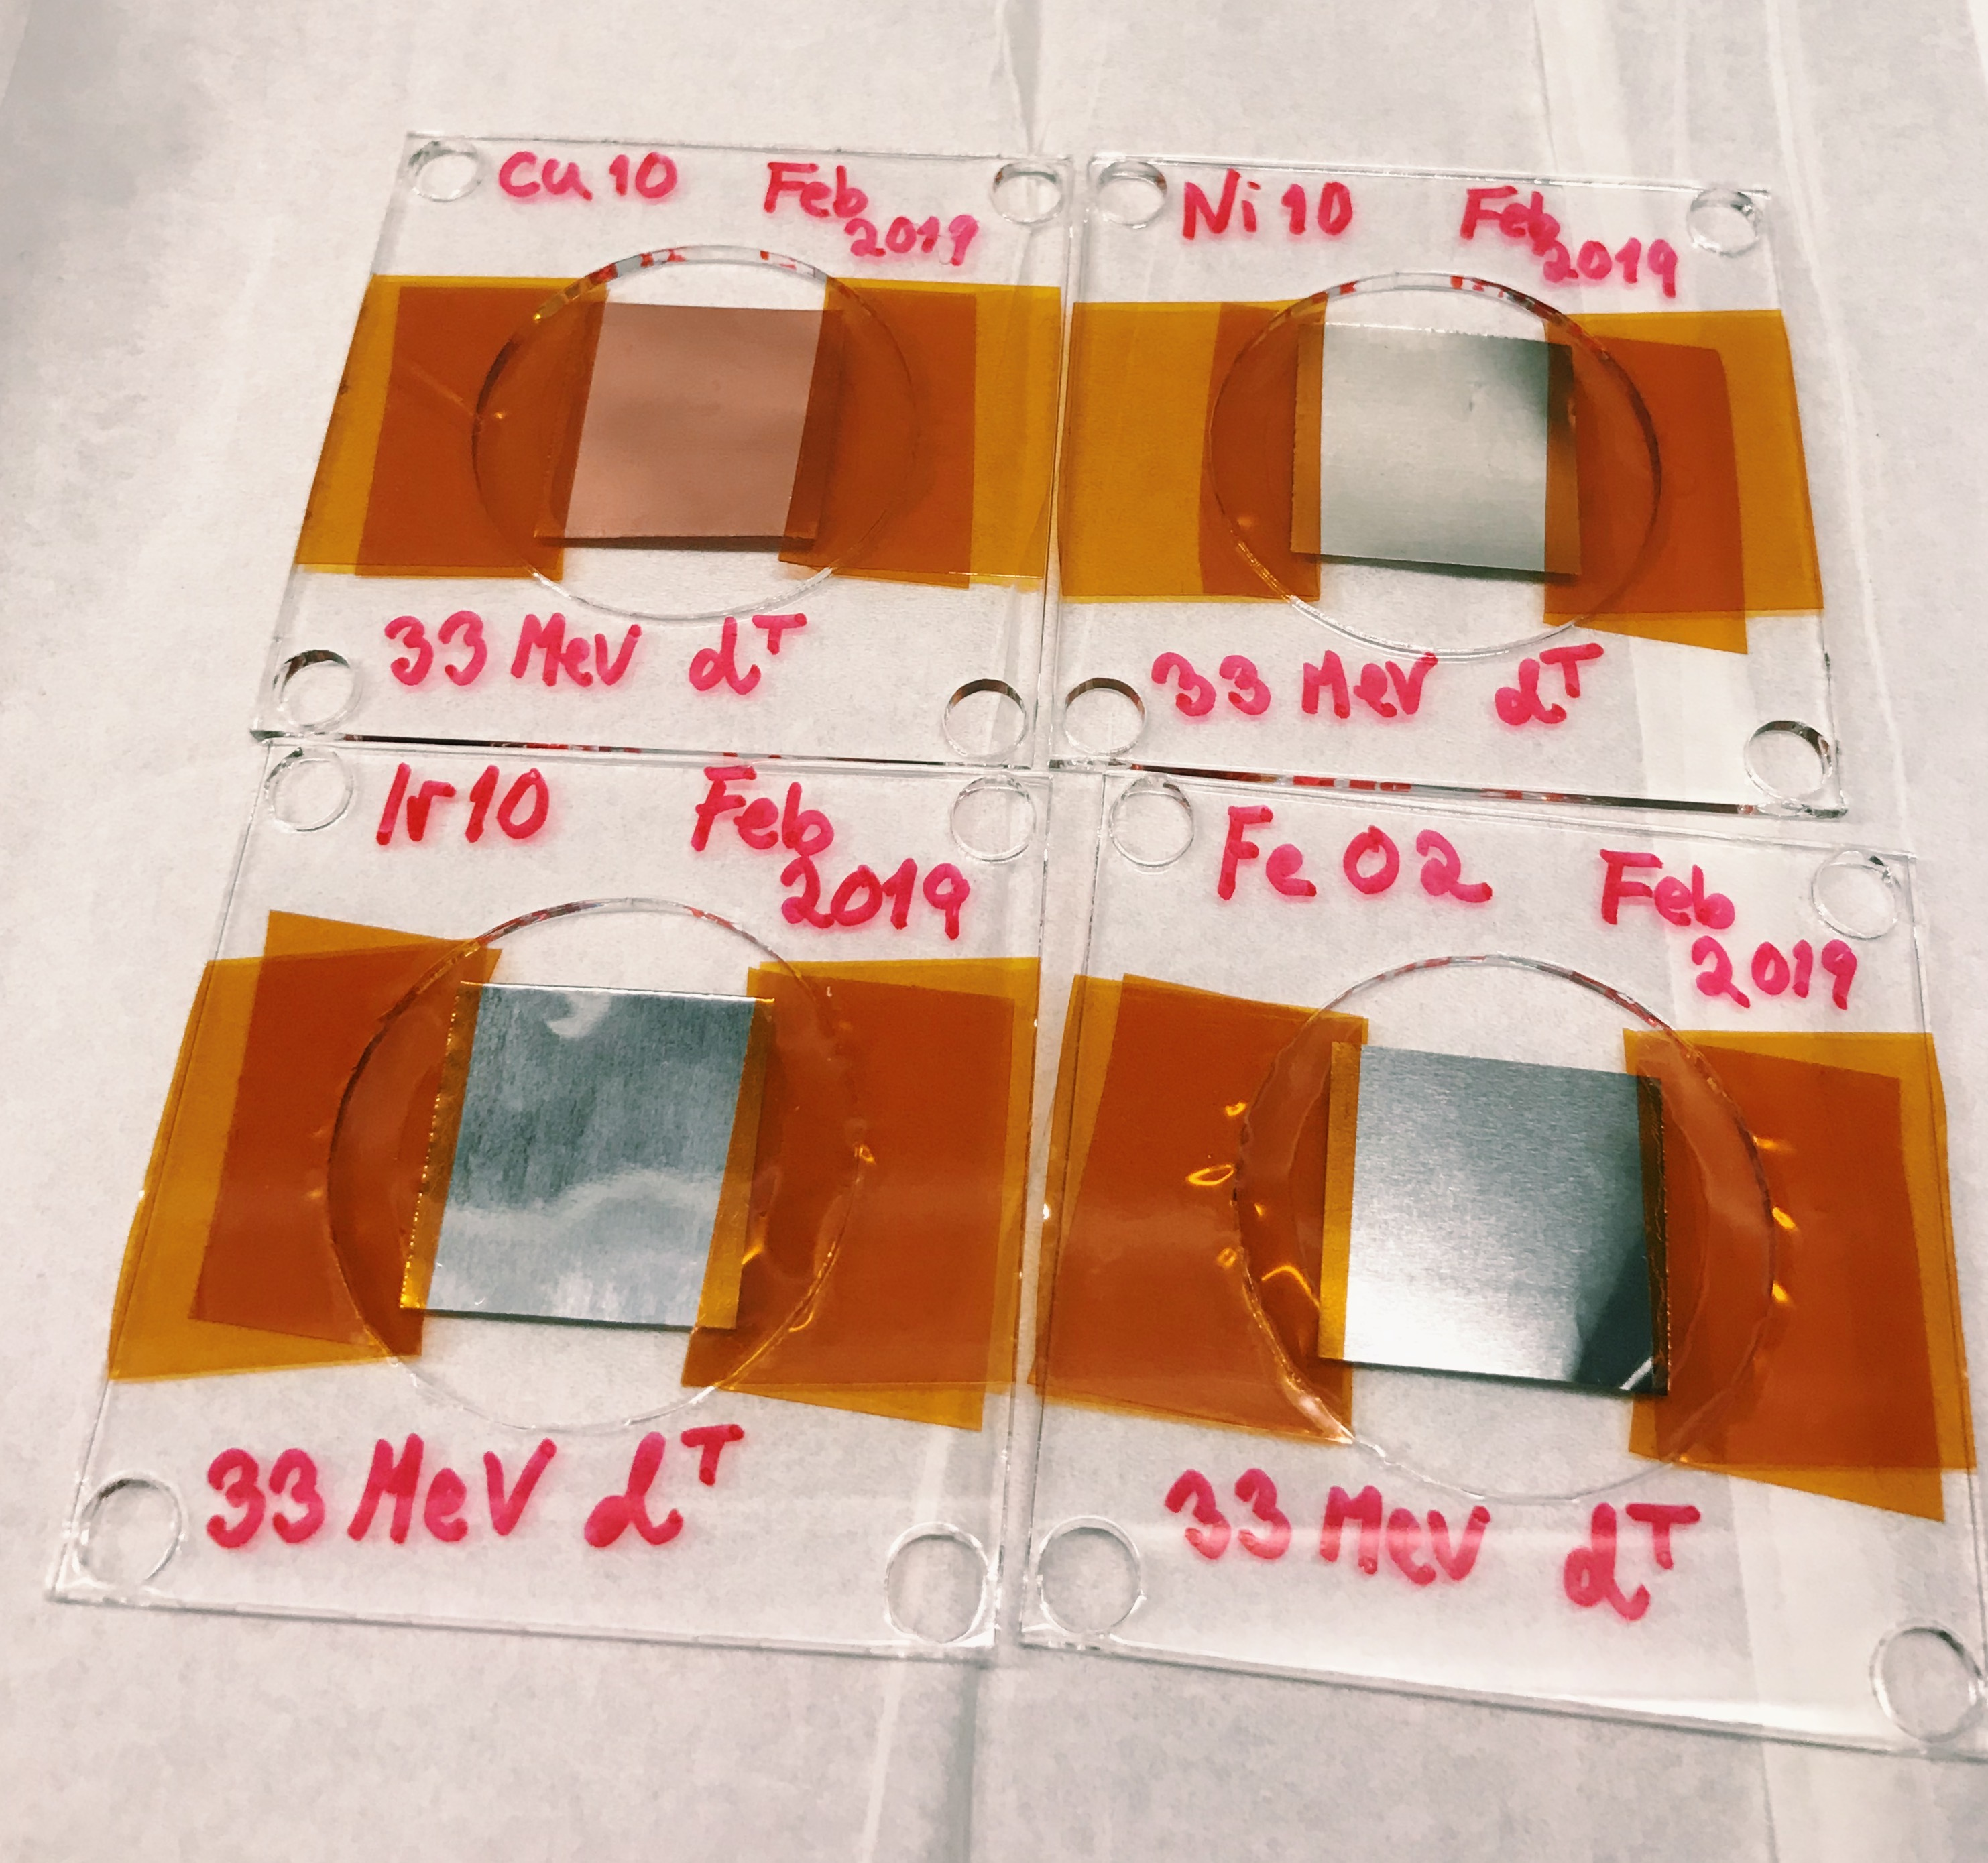
\includegraphics[width=0.5\textwidth]{Experiment/targets_on_frame.JPG}
    \caption{The figure shows the four different targets mounted on plastic frames with a hollow center with capton tape attached along the edges of the foils.}
    \label{fig:targets_on_frame}
\end{figure}


\begin{table}[h!]
%\centering
\caption{Characterization of each foil, along with calculated mass density. Each length is measured in mm, and mass in grams. *: measured from previous experiments}
\label{table:foil_characterization}
\small
\begin{tabular}{lllllll}
\makecell{\textbf{Foil}} & \makecell{Length1 (mm)}  &  \makecell{Length2 (mm)} & \makecell{Thickness (mm)} & \makecell{Mass (g)} & \makecell{\textbf{Mass density (mg/cm$^2$)}} \\ 
\hline
\makecell{SS1} & \makecell{} & \makecell{} & \makecell{} & \makecell{} & \makecell{100.199^*} \\
\hline
\makecell{Ni01} & \makecell{25.228} & \makecell{25.293} & \makecell{0.0285} & \makecell{0.1453} & \makecell{22.772 $\pm$ 0.138} \\
\makecell{Ir01} & \makecell{24.943} & \makecell{24.968} & \makecell{0.0295} & \makecell{0.3436} & \makecell{55.174 $\pm$ 0.053} \\
\makecell{Cu01} & \makecell{25.553} & \makecell{24.883} & \makecell{0.0341} & \makecell{0.1420} & \makecell{22.338 $\pm$ 0.048} \\
\makecell{Fe01} & \makecell{24.400} & \makecell{26.068} & \makecell{0.0278} & \makecell{0.1274} & \makecell{20.030 $\pm$ 0.110} \\
\hline
\makecell{Ni02} & \makecell{25.288} & \makecell{25.428} & \makecell{0.0295} & \makecell{0.1487} & \makecell{23.118 $\pm$ 0.096} \\
\makecell{Ir02} & \makecell{24.923} & \makecell{25.005} & \makecell{0.0278} & \makecell{0.3465} & \makecell{55.601 $\pm$ 0.238} \\
\makecell{Cu02} & \makecell{25.443} & \makecell{25.550} & \makecell{0.0348} & \makecell{0.1451} & \makecell{22.325 $\pm$ 0.028} \\
\makecell{Fe02} & \makecell{25.525} & \makecell{23.800} & \makecell{0.0274} & \makecell{0.1216} & \makecell{20.017 $\pm$ 0.034} \\
\hline
\makecell{Ni03} & \makecell{25.295} & \makecell{25.210} & \makecell{0.0270} & \makecell{0.1425} & \makecell{22.338 $\pm$ 0.066} \\
\makecell{Ir03} & \makecell{24.885} & \makecell{24.983} & \makecell{0.0243} & \makecell{0.3459} & \makecell{55.643 $\pm$ 0.121} \\
\makecell{Cu03} & \makecell{25.560} & \makecell{25.508} & \makecell{0.0343} & \makecell{0.1455} & \makecell{22.313 $\pm$ 0.043} \\
\makecell{Fe03} & \makecell{26.113} & \makecell{25.235} & \makecell{0.0310} & \makecell{0.1315} & \makecell{19.948 $\pm$ 0.114} \\
\hline
\makecell{Ni04} & \makecell{25.303} & \makecell{24.888} & \makecell{0.0273} & \makecell{0.1304} & \makecell{20.704 $\pm$ 0.068} \\
\makecell{Ir04} & \makecell{24.960} & \makecell{24.833} & \makecell{0.0261} & \makecell{0.3471} & \makecell{56.000 $\pm$ 0.109} \\
\makecell{Cu04} & \makecell{25.153} & \makecell{25.603} & \makecell{0.0333} & \makecell{0.1435} & \makecell{22.284 $\pm$ 0.027} \\
\hline
\makecell{Ni05} & \makecell{25.325} & \makecell{25.495} & \makecell{0.0263} & \makecell{0.1406} & \makecell{21.768 $\pm$ 0.045} \\
\makecell{Ir05} & \makecell{24.948} & \makecell{24.958} & \makecell{0.0256} & \makecell{0.3435} & \makecell{55.161 $\pm$ 0.081} \\
\makecell{Cu05} & \makecell{25.213} & \makecell{25.573} & \makecell{0.0334} & \makecell{0.1447} & \makecell{22.443 $\pm$ 0.028} \\
\hline
\makecell{Ni06} & \makecell{25.530} & \makecell{25.195} & \makecell{0.0285} & \makecell{0.1471} & \makecell{22.861 $\pm$ 0.123} \\
\makecell{Ir06} & \makecell{24.760} & \makecell{24.960} & 
\makecell{0.0240} & \makecell{0.3444} & \makecell{55.731 $\pm$ 0.088} \\
\makecell{Cu06} & \makecell{25.343} & \makecell{25.513} & \makecell{0.0340} & \makecell{0.1448} & \makecell{22.396 $\pm$ 0.012} \\
\hline
\makecell{Ni07} & \makecell{25.338} & \makecell{25.278} & \makecell{0.0268} & \makecell{0.1479} & \makecell{23.092 $\pm$ 0.078} \\
\makecell{Ir07} & \makecell{24.955} & \makecell{25.008} & \makecell{0.0278} & \makecell{0.3538} & \makecell{56.685 $\pm$ 0.085} \\
\makecell{Cu07} & \makecell{25.625} & \makecell{25.248} & \makecell{0.0326} & \makecell{0.1444} & \makecell{22.320 $\pm$ 0.014} \\
\hline
\makecell{Ni08} & \makecell{25.205} & \makecell{24.950} & \makecell{0.0256} & \makecell{0.1409} & \makecell{22.409 $\pm$ 0.124} \\
\makecell{Ir08} & \makecell{24.723} & \makecell{24.985} & \makecell{0.0281} & \makecell{0.3585} & \makecell{58.030 $\pm$ 0.130} \\
\makecell{Cu08} & \makecell{25.370} & \makecell{24.885} & \makecell{0.0333} & \makecell{0.1414} & \makecell{22.401 $\pm$ 0.033} \\
\hline
\makecell{Ni09} & \makecell{25.220} & \makecell{25.378} & \makecell{0.0257} & \makecell{0.1392} & \makecell{21.741 $\pm$ 0.073} \\
\makecell{Ir09} & \makecell{24.670} & \makecell{24.993} & \makecell{0.0273} & \makecell{0.3494} & \makecell{56.669 $\pm$ 0.043} \\
\makecell{Cu09} & \makecell{25.390} & \makecell{26.455} & \makecell{0.0331} & \makecell{0.1506} & \makecell{22.425 $\pm$ 0.041} \\
\hline
\makecell{Ni10} & \makecell{25.285} & \makecell{24.405} & \makecell{0.0271} & \makecell{0.1425} & \makecell{23.093 $\pm$ 0.024} \\
\makecell{Ir10} & \makecell{24.973} & \makecell{24.980} & \makecell{0.0270} & \makecell{0.3435} & \makecell{55.065 $\pm$ 0.055} \\
\makecell{Cu10} & \makecell{25.470} & \makecell{25.338} & \makecell{0.0355} & \makecell{0.1440} & \makecell{22.314 $\pm$ 0.047} \\
\hline


\hline
\makecell{SS2} & \makecell{} & \makecell{} & \makecell{} & \makecell{} & \makecell{100.865^*} \\
\makecell{P-degrader} & \makecell{} & \makecell{} & \makecell{} & \makecell{} & \makecell{1900.0^*} \\
\makecell{Ni neutron monitor} & \makecell{} & \makecell{} & \makecell{} & \makecell{} & \makecell{\textbf{?}} \\
\hline
\end{tabular}
\end{table}










\section{Lawrence Berkeley National Laboratory's 88" Cyclotron} \label{sec:LBNL-88}

Lawrence Berkeley National Laboratory (LBNL) \cite{KireeffCovo2018a}  is a national research laboratory on behalf of the U.S. Department of Energy through its Office of Science, and is operated by University of California, Berkeley. LBNL was founded by Ernest Orlando Lawrence, the inventor of the cyclotron, in 1931 \cite{webpage-lab-about}. The 88-Inch Cyclotron has a cyclotron number of K=140, and can accelerate both light and heavy ions up to Uranium.  \cite{webpage-lab}. The cyclotron has many purposes,  The researchgroup which does isotope production at the facility works with development of nuclear reaction data, along with researching production methods of medically valuable radionuclides. There are multiple other programs that takes place in the facility which include chip testing and space effects testing, super heavy element searches, fundamental nuclear structure measurements, novel scintillation characterization, fission yield and neutron inelastic scattering measurements (GENESIS). \\ %The cyclotron number is the maximum kinetic energy which can be reached for protons (with no relativistic factors taken into account). The maximum kinetic energy a particle can gain is found from the cyclotron number:%\begin{equation}
%    \frac{E_k}{A}=K\Big(\frac{Q}{A}\Big)^2
%\end{equation}
%For deuterons with mass number A=2 and charge Q=1, the maximum kinetic energy is $E_k=70$ MeV. 


\noindent 
A cyclotron is a device that accelerates positively charged particles. It is operated by an alternating (radiofrequency) electric field, and a perpendicular magnetic field, which by the Lorentz Force forces the particle to accelerate in an outward spiral. The 88-Inch cyclotron is an isochronus cyclotron, with a magnetic field that increases with radius. The ions which are accelerated are produced by ECR ion sources and injected into the cyclotron %\cite{KireeffCovo2018a}. 
The facility is figured in \ref{fig:LBNL_88}, and consists of a cyclotron vault and experimental caves, where cave 01/02 is where the irradiation of the target stack took place. Cave 4C is today used for gamma-ray spectroscopy, where 6 of a total of 7 high purity germanium detectors which were used in this work were located. Faraday cups can measure the beam current at different steps along the beamline. %Faraday cups are dense metal block, usually 6-7 cm broad Copper and Tantilum. The Faraday cups work as a beam stopper,
%Since we know the initial number of particles accelerated, and the cup is electrically isolated. Since electrons close to the surface can be scattered of, it can read of higher positive charge than what is correct. Therefor, a magnet surrounds the cup to bend the electrons back to the Faraday cup in what is called magnetic suppression. 
From the cyclotron vault, the beam is directed and focused to the correct cave with bending magnets and quadrupole magnets. From de-acceleration of the beam particles, some particles are lost and the transmission efficiency can be calculated by comparing the current at the Faraday cup right after (BS-02) the particles have gained the desired energy, and current at the Faraday cup right before the particles are in the end of the beamtube of cave 01/02 (FC-01) can be measured.  


%\begin{figure}
%    \centering
%    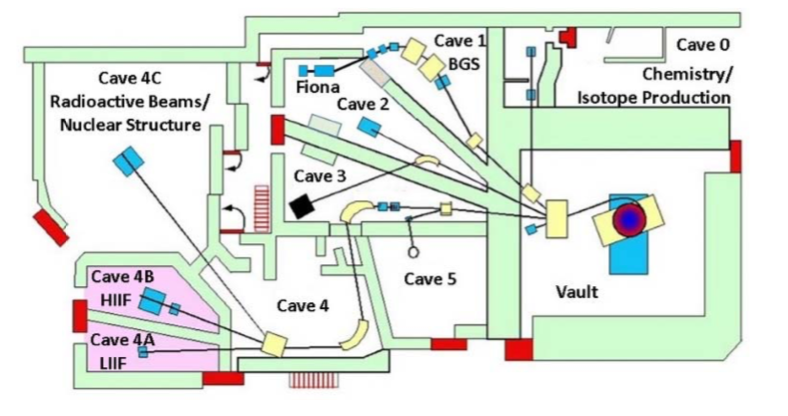
\includegraphics[width=0.8\textwidth]{Experiment/LBL_88.png}
%    \caption{An overview of the 88" Cyclotron facility. https://cpb-us-e1.wpmucdn.com/sites.usc.edu/dist/7/89/files/2018/04/133-18q03um.pdf }
%    \label{fig:LBNL_88}
%\end{figure}

\begin{sidewaysfigure}[ht]
    \centering
    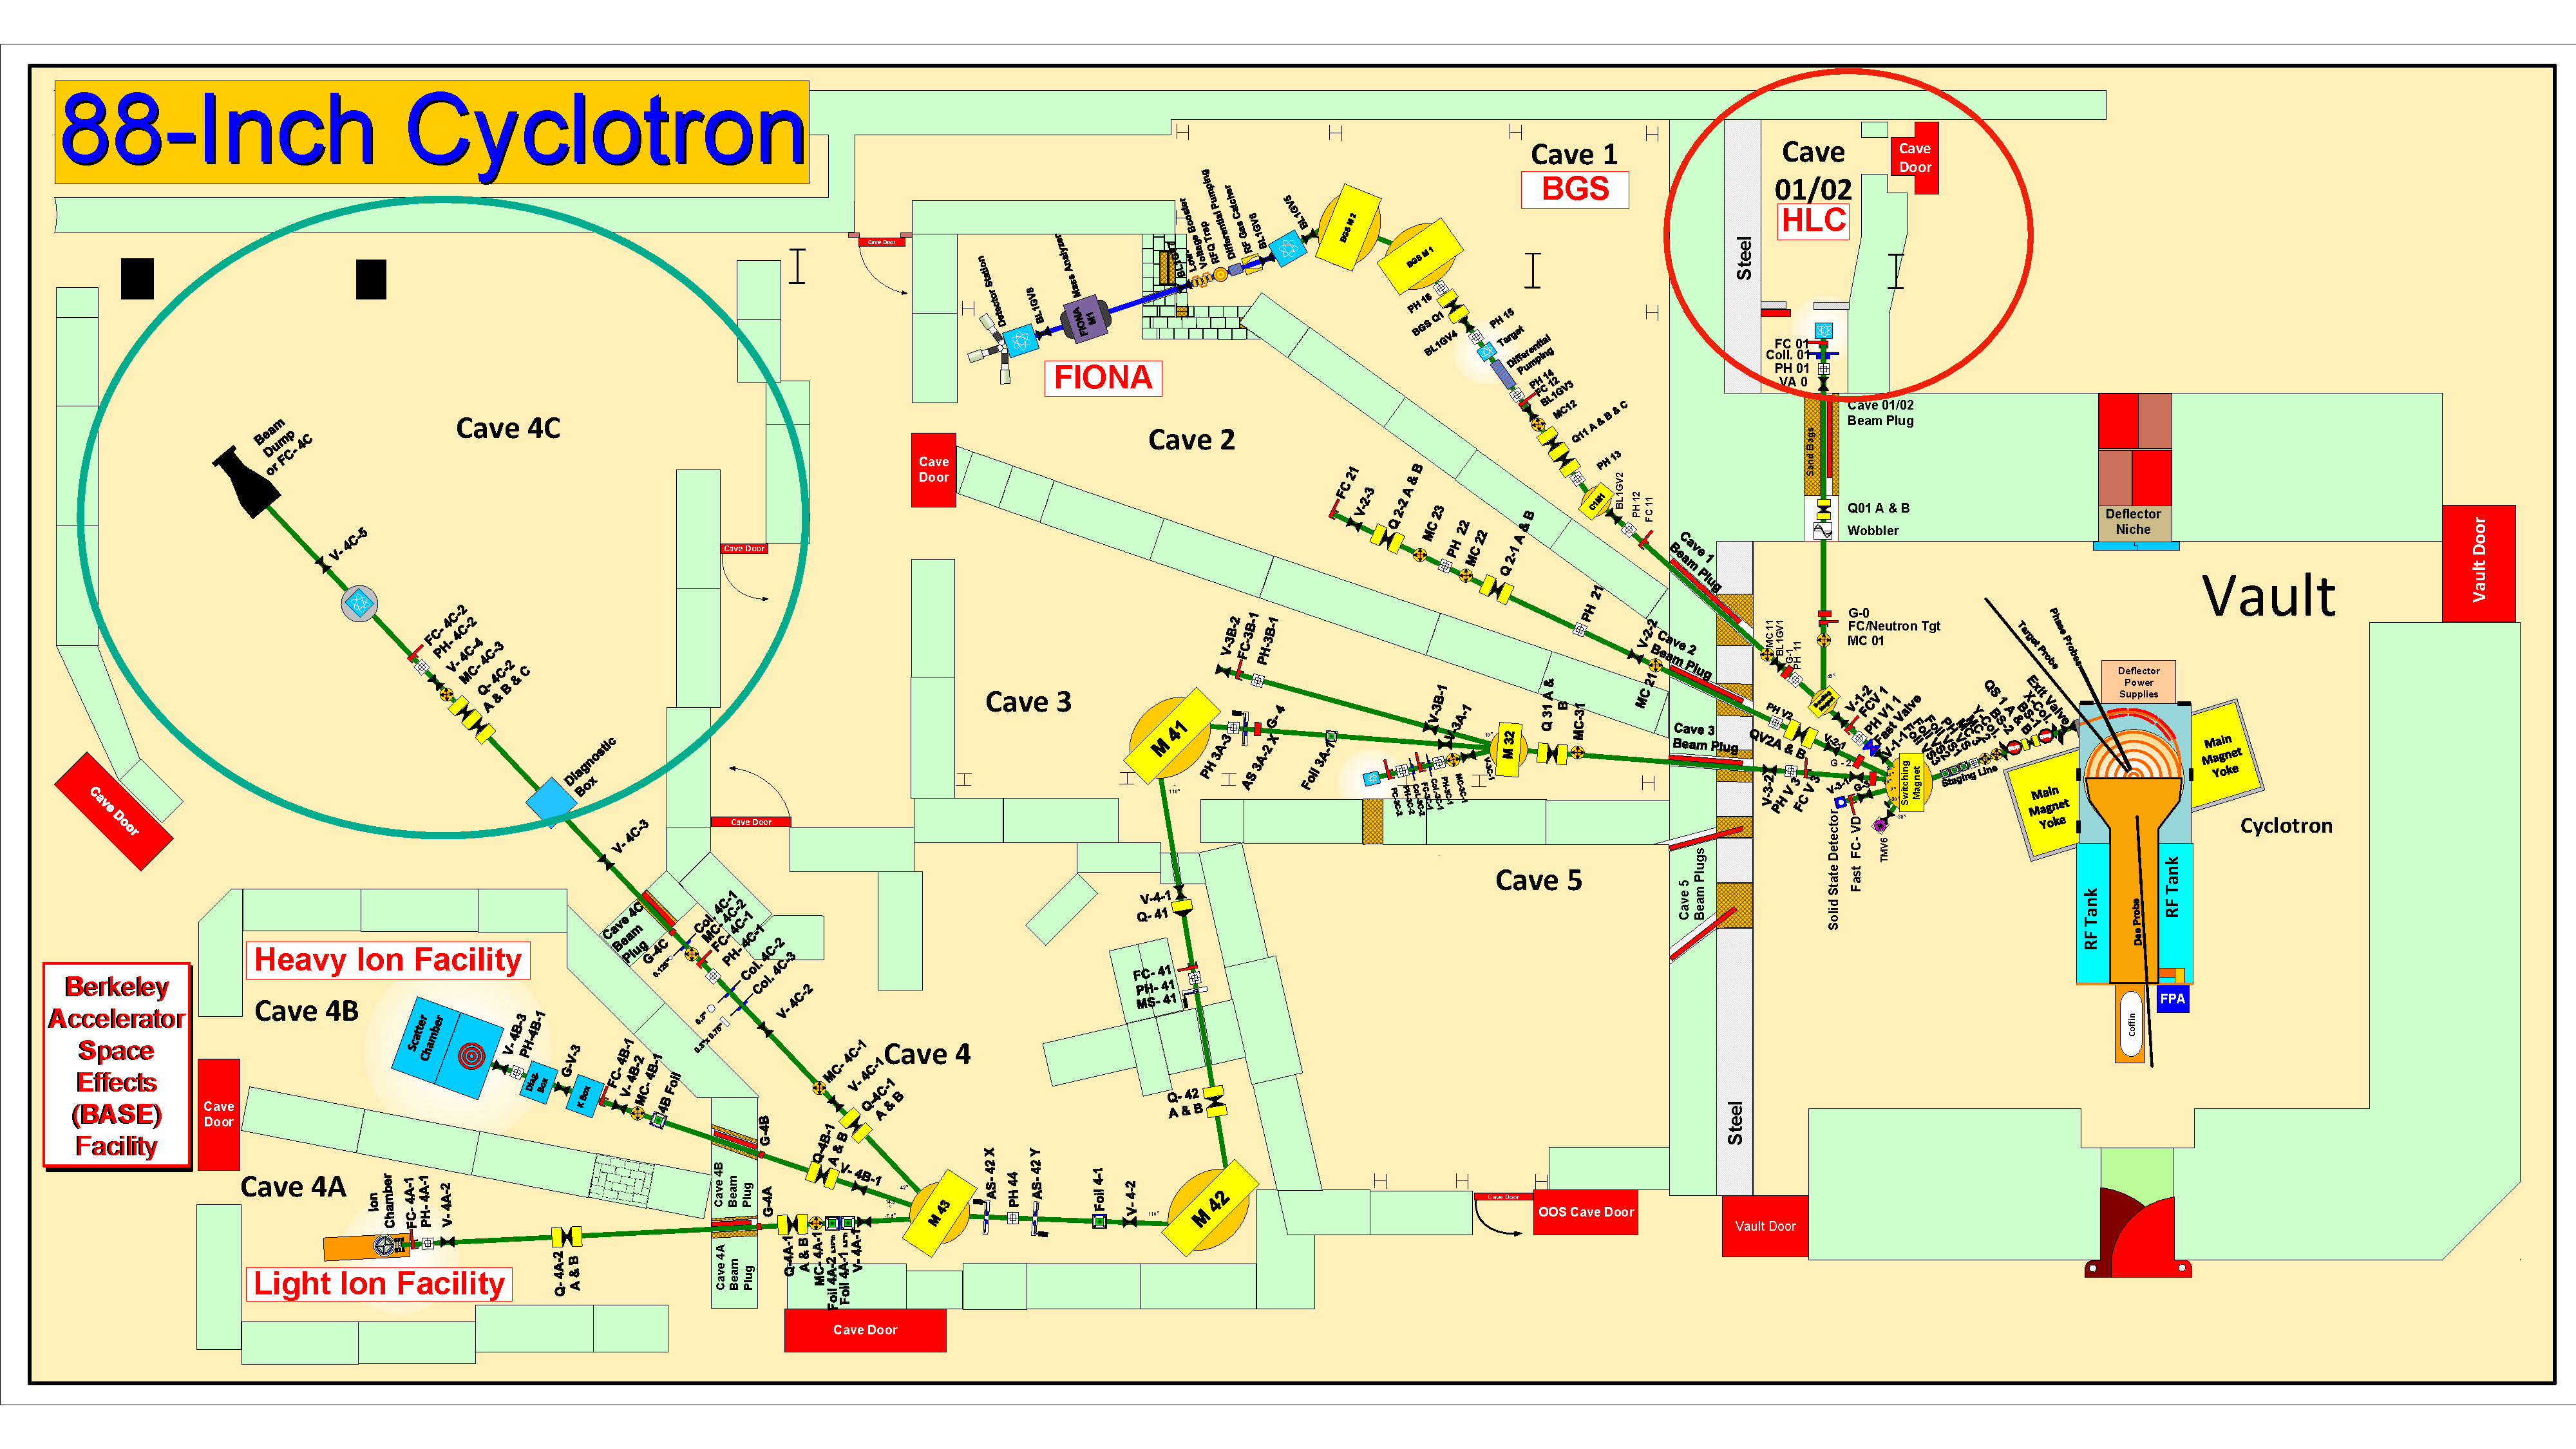
\includegraphics[width=1\textwidth]{Experiment/Control-Room-Map-new.pdf}
    \caption{An overview of the 88" Cyclotron facility. The facility have several isolated beamlines that can be used for irradiation in the experimental caves. The irradiation of the target stack took place in cave 01/02 (red circle), while some of the detectors used in the gamma-rays spectroscopy was located in cave 4C (green circle) which is no longer used as an irradiated chamber. Bending magnets are used to steer the beam into the desired beamline, and focusing quadropole magnets are used to focus the beam in the cyclotron vault. }
    \label{fig:LBNL_88}
\end{sidewaysfigure}

\section{High purity Gerganium detector} \label{sec:detector_calibration}
\noindent  

For the gamma-ray spectroscopy, seven different high purity germanium detectors with coaxial right cylinder geometry were used. Six mechanically cooled p-type IDM Ortec detectors (detectors 1-6) with detector diameter 85 mm, detector length 30 mm, hole depth 15 mm and hole diameter 9 mm. The detector volume was 169.996 cm$^2$ (assuming detector hole cylindrical). The outside contact layer was doped with lithium, and the hole contact layer with boron. In addition one liquid-nitrogen cooled n-type \textcolor{red}{ORTEC GMX series (mode: GMX-50220-S)} Germanium detector which also had a thin beryllium window for improved x-ray efficiency (detector 7), with detector diameter 64.9 mm, detector length 57.8 mm, hole diameter 9.4 mm and hole depth 48.6 mm. The detector volume was 190.365 cm$^{2}$. The outside contact layer was doped with boron and the hole contact layer was doped with lithium. \\

\noindent 
The high purity Germanium detector is a type of semiconductor, which is a material where the energy required to remove an electron from the valence band (in the outer atomic shell) to the conduction band is small. The germanium atom has atomic number 32, and 4 valence electrons in the outer p4 shell \textcolor{red}{(need citation?)}. The atoms in the detector are bound through covalent bonds in a crystal structure. The main mechanism of a semiconductor is creation of electron-hole pairs after energy deposition of an ionizing particle in the crystal. If an electron is excited to the conduction band, a hole is left. This hole can move as a neighboring electron fills this spot, leading to a chain reaction, as the hole will move in the crystal. Both the electron in the conduction band and the hole in the valence band contributes to an electric current (\cite{Leo1994}, p. 215-216). \\ The major advantage with semiconductor detector is that the average energy to create an electron-hole pair is very low, which results in a superior energy resolution in comparison to other detectors like gas and scintillation detectors. At 77K, the average energy is 2.96 eV to create an electron-hole pair (\cite{Leo1994}, p. 228).  High energy resolution is important, dependent on the energy difference of two close lying gamma-peaks and the resolution, the two peaks can be distinguished. For 1000 keV, the resolution of a Germanium detector is 0.1\%, which means that it is possible to separate two gamma-ray peaks within ca. 1 MeV (\cite{Leo1994}, p. 117). \\

\noindent 
The detectors are doped to create an imbalance in the number of holes and electrons in the conduction band in a pure crystal (\cite{Leo1994}, p. 220), either by creating an excess of holes by adding a an acceptor of electrons (p-type) or by adding a donor of electrons so there is an excess of electrons (n-type). In reality, both dopants are present (so there is a p-n junction), but the dopant with the highest occurance has the highest probability of interacting with radiation. The n-type material will have more electrons which will move toward the p-type material, and visa versa. Therefor, an imbalance arises due to the p-type having an access electrons, and the n-type having an access of holes near the equilibrium. The region where there is an imbalance is called the depletion zone, and a potential across the junction arises. When electrons from p-type or holes from n-type comes near the depletion zone (which diffuses towards the side with the opposite charge), will be swiped back due to the equal charge on the depletion zone. This will create a voltage current which is assigned to a channel number as a count. The gap is quite narrow, but when a bias voltage voltage is applied between the inner and outer radii of the detector cylinder, the depletion zone width increases. With this diffusion of electrons and holes process, the surface layer becomes heavily doped. The consequence is a thick dead layer which can attenuate or stop radiation before entering the detector volume (\cite{Leo1994}, p. 233).  Figure \ref{fig:ntype_detector} is shows the principle of a n-type coaxical cylinder detector. Where the inner hole as an overweight in positive charges, and the electrons resulting from an incident ionizing particle diffuses towards the hole. \\

%With the diffusion process, the surface layer becomes heavily doped, so that the depletion layer extends mainly into the p-side. This, unfortunately, leaves a relatively
%thick dead layer through which radiation must pass before reaching the sensitive volume.
%For energy measurement, this is particularly disadvantageous as the energy lost in
%this layer goes unrecorded. (p. 233).  

%In order to obtain a sufficient sensitive thickness for the detection of gamma rays, the first detectors were made from lithium compensated germanium. These detectors are known as Ge(Li) (pronounced as jelly) detectors. Since maximum obtainable thicknesse for compensated germanium are about 15 or 20 mm, a coaxial geometry is generally use to maximize the sensitive volume. This is schematically diagramed in Fig. 10.18. In this configuration, lithium is drifted in from the outer surface of a cylindrical crystal of p-type germanium to form a cylindrical shell of compensated material. A central core of insensitive p material is then left. If this core extends along the entire length of the axis, the configuration is then known as a true coaxial or open-ended coaxial detector. To increase sensitive volume even further, lithium may also be drifted infrom the front face of the cylinder. The extent of the insensitive core is then reduced.These are known as closed-end coaxial detectors. For high counting efficiency, the central core may also be removed to form a well type detector. The various configurations are illustrated in Fig. 10.18. For lower gamma energies, Ge(Li) detectors may also be fabricated with the conventional planar geometry. Because of the high mobility of the lithium ions in germanium, even at room temperature, Ge(Li) detectors must be kept at liquid nitrogen temperatures at all times.(p. 239)

%The sensitivity of coaxial Ge(Li) detectors is generally limited by the thickness of
%the dead layer formed on the face of the crystal by lithium drifting and the cryostat
%window which absorb low-energy photons (p. 240). 



%At room temperature, thermal
%energy can excite the electron from the valence to the conduction band and cause noise in spectra. 
%Therefor, Germanium detectors are operated at temperatures close to 0 Kelvin. The detectors are doped to create an imbalance in the number of holes and electrons in the conduction band in a pure crystal (\cite{Leo1994}, p. 220), either by creating an excess of holes by adding a an acceptor of electrons so that there is an excess of holes (p-type) or by adding an donor of electrons so there is an excess of electrons (n-type). In reality, both dopants are in the detector, but what is most there is what decides what it is. \textcolor{red}{add the oposite material in the detector, (p-type detector with n-type material) and apply bias voltage so that } Based on how Germanium detector is doped, when adding a biasvoltage across the inner hole to the outer radii of the cylinder, a depletion layer rises. The bias voltage determines the thickness of the depletion layer, and the volatges can be up to 4500 V for Germnanium detectors.  (The voltage must be increased slowly to reduce the noise.)  \cite{Leo1994}, p. 243. In addition, 

\noindent 
The efficiency of a detector is the number of events registered divided by the events emitted by the source. The absolute efficiency can be divided into intrinsic and geometrical efficiency, where the intrinsic efficiency is the number of events registered by the number of events hitting the detector. The intrinsic efficiency thus depends on the interaction cross section between the incident particle and the detector material, \textcolor{red}{and as described above, the IDM's having a larger surface, the geoemtrical efficiency is larger}. For neutral particles like photons, the size affects the intrinsic efficiency, as the probability of interaction gets larger. The geometrical efficiency is based upon the shape, and is the radiation emitted by the source which hits the detector (\cite{Leo1994}, p. 121-122), and is therefor dependent on the solid angle. The detector volumes were comparable in size. However, due to the former being broader and shorter (higher surface area, and higher solid angle), the relative efficiency of the IDM-detectors are lager (ca. 52\%) than the germanium detector (ca. 20\%). Therefor, the IDM-detectors are more sensitive to background radiation. The IDM-detectors were located in cave 4C (see figure \ref{fig:LBNL_88}), which have previously been used as radiation chamber. Thus, background radiation was present. Detectors 1-6 were used for high efficiency counting of foils. For detector 7, there was led shielding around the detector. In addition, the detector had a slightly higher resolution, and was therefor used for precision measurements%, while IDM used for counting and increasin throughput (how many foils can be counted per unit time) Spectra taken on the Germanium detector. 
The resolution of a detector is defined as the the fwhm of the peak divided by the true gamma-line. Using the 661.657 keV (85.10\%) gamma-line of $^{137}$Cs, the resolution of detector 1 at 10 cm was 0.28\% while it was 0.25\% for detector 7 at 10 cm. \\ %Usually the 1332 keV gammaline of 
%$^{60}$Co is used: However we use Cs137 661.657 (keV ).... because it is a calibration source. For room131 at 5 cm, 0.25 and for hpge at 10 cm 0.28. \\

The duration of a voltage pulse signal takes to construct is important, because other events that occurs meanwhile cannot be registered. This leads to a dead time, which is time where nothing is recorded (\cite{Leo1994}, p. 120). The time that a detector registers an event is called the live time, which is the real time minus the dead time. Ideally, a system that does not add dead time to the existing (non-paralyzable) is preferred to reduce the amount of time where the detector is not detecting. 


%\textcolor{red}{The resolution of a detector is not that good, it is rather Gaussian shaped, with a finite width. The resolution is simply the fwhm of the peak divided by the true gamma-ray energy.}  \\
\noindent
In order to visualize the signal from the detector, Maestro  (Multichannel Analyzer Emulation Software\footnote{https://www.ortec-online.com/products/application-software/maestro-mca}) was used. \\

\begin{figure}
    \centering
    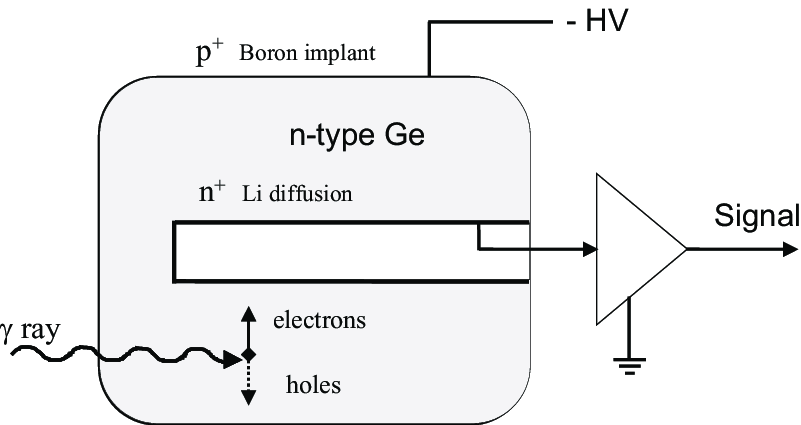
\includegraphics[width=0.8\textwidth]{Experiment/n-type_Ge.png}
    \caption{Figure shows a n-type germanium detector. Since the material is n-type, a potential arises around the boron implant (outer surface). where a p-n junction is created around the boron implant (outer surface). Figure is from \cite{Lee2003}.  %\textcolor{red}{In principle, the p-n junction of a coaxial detector can be located either at the inner or outer surface of the crystal as shown in Fig. 8.6. If the junction is on the outer surface, the depletion region extends inward as the high voltage bias is increased until the crystal is fully depleted. In the opposite case, the depletion region grows outward. The p-n junction at the outer surface requires a much lower full depletion bias and therefore, is preferred.
%The practical electrode configurations of coaxial Ge detectors are shown in Fig. 8.7. To make the p-n junction at the outer surface, the n+ contact is performed over the outer surface for a p-type detector while the p+ contact is applied in case of an n-type crystal. The n-type coaxial detectors are often called reverse electrode detectors. The reverse bias requires a positive outside potential for a p-type and a negative potential for an n-type relative to the central electric potential., \url{https://www.science.mcmaster.ca/radgrad/images/6R06CourseResources/4RA34RB3_Lecture_Note-8_HPGe_Detector.pdf}} due to the charge difference around betwwen the p and n side.  Developments in large gamma-ray detector arrays - Scientific Figure on ResearchGate. Available from: https://www.researchgate.net/figure/Configuration-of-an-n-type-intrinsic-germanium-closed-end-co-axial-detector_fig7_230962552 [accessed 15 May, 2020]}  }
}
    \label{fig:ntype_detector}
\end{figure}
\begin{comment}
\begin{figure}
    \centering
    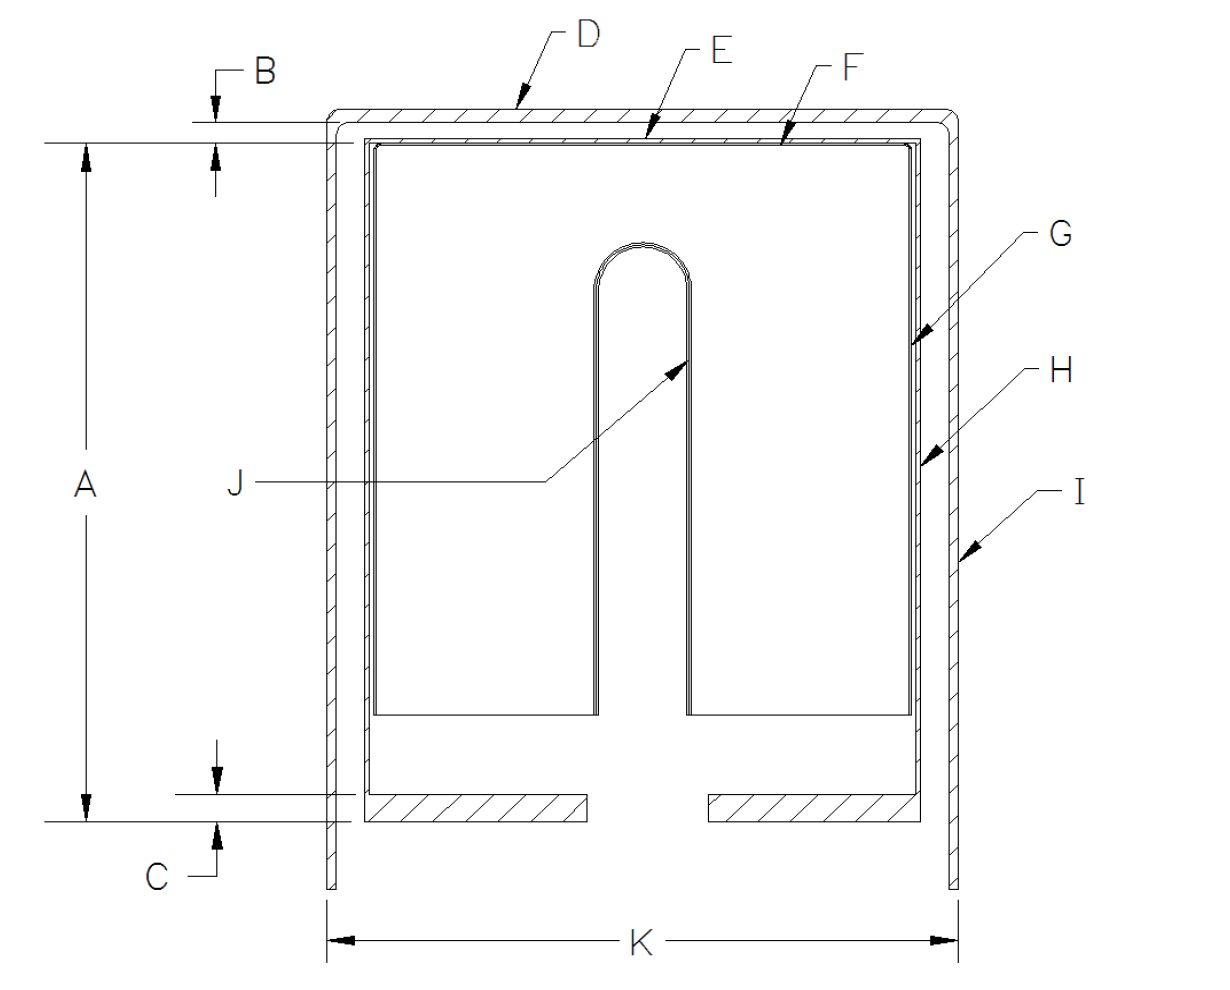
\includegraphics[width=0.8\textwidth]{Experiment/scetch_detector.png}
    \caption{The figure shows a scetch of the detector. The figure is from the detector diagram of IDM. }
    \label{fig:detector_scetch}
\end{figure}
\end{comment}
\subsection{Obtaining a spectrum}

\noindent 
The electrical signal (voltage pulse) registered in a detector has a net-electrical charge which is proportional to the amount of gamma-ray energy which was registered in the detector (\cite{Gilmore2008}, p. 61). The electrical signal is assigned a channel number, which is in accordance with the charge collected. To obtain a spectrum, the number of registered events in each channel is counted, and the well-known peaks of the gamma-ray spectrum rises. Ideally, the peaks would appear as step functions, as the gamma-ray energies are discrete. The counts in the channel close to the channel representing the true peak appears in a histogram which follows a Gaussian shape  (\cite{Gilmore2008}, p. 186). Due to incomplete charge collection (ie. that electrons or holes are not collected), moves counts from the center of the distribution to lower channels, creating a low energy tale of the peak (\cite{Gilmore2008}, p. 135). \textcolor{red}{The shape of the peaks are represented in the following equation as a function of the channel number
\begin{equation}
    \text{peak(x)}= A\cdot \Big[e^{-\frac{(x-\mu)^2}{2\sigma^2}}+ R\cdot e^{\frac{i-\mu}{\alpha \sigma}}\erfc\Big(\frac{1-\mu}{\sqrt{2\sigma}} + \frac{1}{{\sqrt{2\alpha}}} \Big) \Big]
\end{equation} where blablabal..... John papers. Maybe not include because cannot describe.... SHPOULD ALSO INCLUDE HOW THE COUNTS ARE CALCULATED, are those within}  \\

%\textcolor{red}{The  shape  of  the  peak:   The  peak  is  a  histogram  that  approximate  a  Gauss  curve  (p.   186).Peak searching (SAMPO) using first and second order derivatives to search for peaks (p.185) Due toincomplete charge collection (that electron or holes are not collected) no matter how caused movescounts from the centre of the Gaussian distribution to lower channels, creating a low energy tale tothe peak (p.135)  \cite{Gilmore2008}} 


The observed gamma-peaks in the spectra obtained in this work are results of beta-decay where the observed gamma-rays are from the decay of the excited daughter nucleus, or gamma-rays from decay of isomeric states. If two nuclei feeds into the same daughter nucleus, the possibility of populating the same energy level is present.\\

\noindent 
In a detector, the main interactions of gamma-rays and X-rays are via the photoelectric effect, Compton scattering and pair production (\cite{Leo1994}, p. 53).  As described in section \ref{sec:particle_interactions}, photons are attenuated exponentially as a function of depth of medium and the absorption coefficient of the medium, but not degraded in energy (equation \ref{eq:photon_attenuation}). Therefor, the gamma-radiation is highly penetrating, and some gamma-rays will also escape the detector volume. Therefore, large detector volumes are desired, to increase chances of all radiation being deposited in the detector ( \cite{Gilmore2008} p. 32). The attenuation coefficient is the sum of all the possible interactions (including Raleigh and Klein-Nishina scattering). In a detector, photopeaks are desired, where all the photon energy is deposited within the detector.  \\ 
\noindent 
Photoelectric effect occurs when a photon is completely absorbed by an atomic electron, and this effect dominates at low photon energies. This effect is desired in gamma-ray spectroscopy, as all the total energy of the gamma-ray will be registered in one photopeak. The probability of photoelectric effect is proportional to the $Z^{4 \text{ or } 5}$, and inversely proportional to the gamma-ray energy. Therefor, a high Z-material is desired to increase the probability

\begin{equation}
    \tau \propto \frac{Z^n}{E_\gamma^{3.5}}, \quad n=4,5
\end{equation}

\noindent

\noindent In Compton scattering, the photon transfers parts of its energy to an assumed electron at rest, and is scattered with an angle $\theta \in (0^\circ, 180^\circ)$. Dependent on the angle, the energy of the deflected photon will vary, and give a spectrum of different energies, where higher scattering angle transfers more energy to the recoil electron. If the final photon escapes the detector, the count will not appear close to the photopeak, but instead contribute to a Compton continuum. The probability of Compton scattering is proportional to the detector Z-value

\begin{equation}
    \sigma \propto Z
\end{equation}

\noindent 
In pair production, the photon is transformed into an electron-positron pair in a nuclear or electric field. Because of this, the energetic threshold is two electron restmasses, of 1.022 MeV. The electron will be registered as an event, and the positron will quickly annihilate with an atomic electron. If both are registered, the peak will appear at the initial gamma-ray energy, if not, we will have a single escape peak at $E_\gamma-511$ keV or double escape peak at $E_\gamma-1022$ keV. Probability increases with Z of detector material squared 

\begin{equation}
    \kappa\propto Z^2
\end{equation}

%(\cite{Leo1994}, p. 54-59). \textcolo{red}{The total attenuation coefficienct adds the different probabilities and gives a function which... }

In addition, interaction via detector shielding occurs, which can lead to emission of characteristic X-rays from the absorbing medium (typically led). Also, since the shielding material is dense, most gamma-rays from Compton scattering are backscattered, and if scattered by more than 120$^\circ$ appears as a broad peak within 200-300 keV. In addition, an annihilation peak at ca. 511 keV is often present, and appears as either a result of pair production in the shielding, where only one gamma-ray will be detected (since they are emitted in opposite directions), or the possibility of annihilation of the positron of a $\beta^+$-emitter (\cite{Gilmore2008} p. 34-35). Pileup is an effect which appears due to random summing which is due to possibility of two gamma-rays being detected simultaneously (\cite{Gilmore2008} p. 33). Figure \ref{fig:gammarayspectrum_example} shows an example of a gamma-ray spectrum for Ir05 ($E_d\approx 21 $ MeV) approximately 35 hours after end of beam on a logarithmic scale. The background at low energies is higher due to the multiple Compton continuum which are added together. In addition, the pileup effect can be seen on the high-end side of the spectrum. \\


\begin{figure}
    \centering
    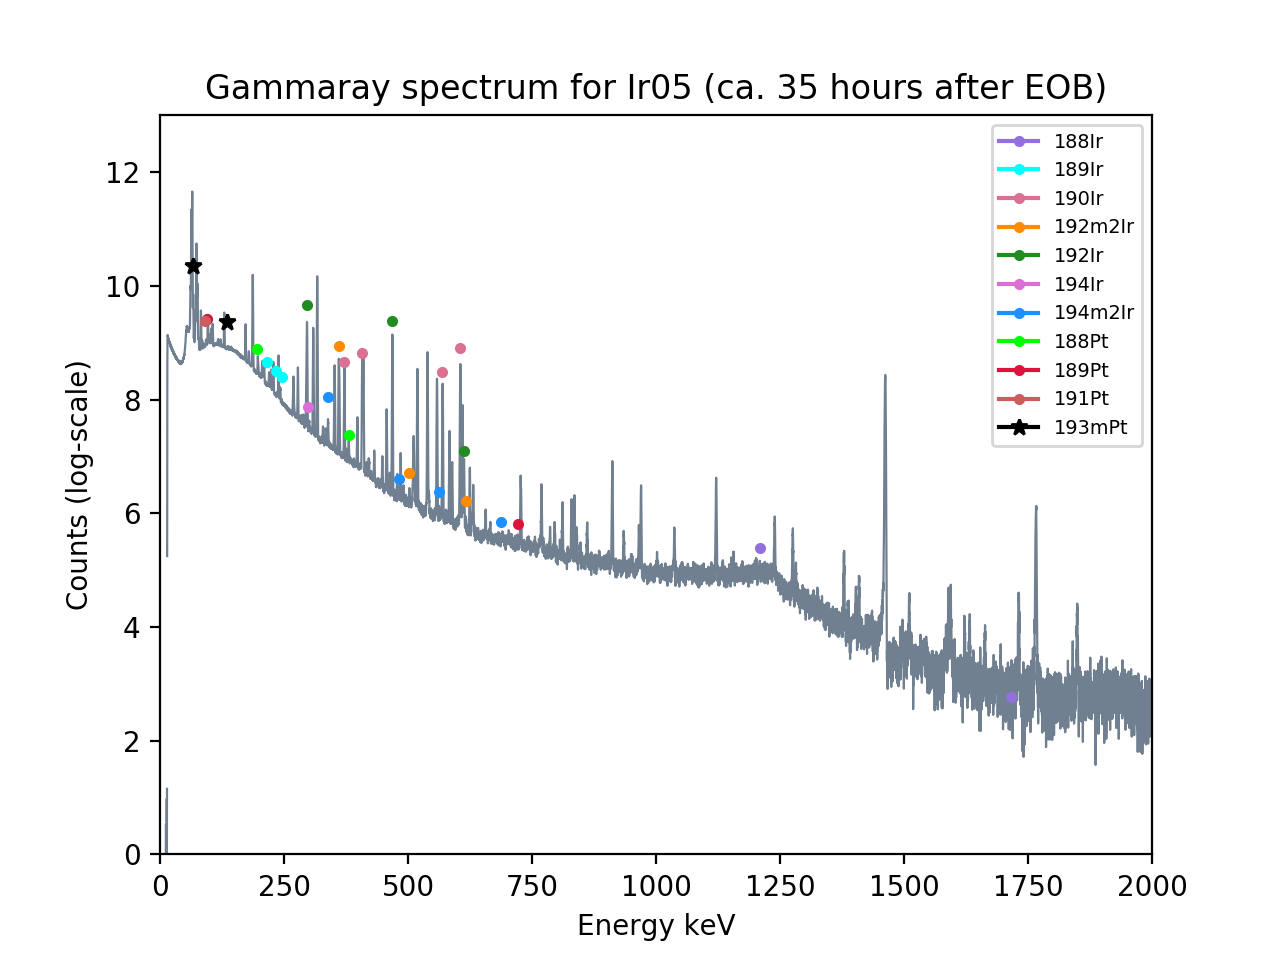
\includegraphics{Analysis/gammaray_spec_Ir05.png}
    \caption{Gamma-ray spectrum for Ir05 (with deuteron energy ca. 21 MeV) taken approximately 35 hours after end of beam. Nuclei does not necessarily represent what is present in the spectrum, but where the peak would have been. Hard to include all since there are different decay times.}
    \label{fig:gammarayspectrum_example}
\end{figure}


\noindent 
Ionizing radiation statistics is based upon Poisson statistics, where the probability of observing N events is a discrete value

\begin{equation}
    P(N)=\frac{\mu^N e^{-\mu}}{N!}
\end{equation}

where $\mu$ is the mean value, which is equal to the variance ($\mu=\sigma^2$). This distribution is valid when the probability is small \textcolor{red}{(decay probability small?)} and the number of trials (\textcolor{red}{number of decays?}) are large (\cite{Leo1994}, p. 85).  The distribution is not symmetric, but as the mean value increases, the peak approximates a Gaussian shape. Therefor the peak is assumed Gaussian with an exponential skew towards lower energies which is caused by incomplete charge collection, along with a step function which takes the background into account. The area of the whole peak is net net number of counts which is necessary to obtain an activity in the foil. The statistical uncertainty arises from the Poisson statistics, and is large if net number of counts are low:

\begin{equation}
    \sigma N_i = \sqrt{N_i}
\end{equation}

Therefor, to reduce the statistical uncertainty, a relative uncertainty of less than 1\% is preferred ($\frac{\sigma N_i}{N_i}\frac{1}{\sqrt{N_i}}=1\%$) 
The systematic uncertainty is in the detector, caused by a process called annealing. \textcolor{red}{write about it??} \\




\noindent 
In this work, the gamma-ray spectra were analyzed in FitzPeaks \cite{Fitzgerald2009}. The mathematical algorithm inwhich Fitzpeaks in based on is SAMPO80\cite{Koskelo1981}. \textcolor{red}{Peak searching (SAMPO) using first and second order derivatives to search for peaks \cite{Gilmore2008} (p.185)}  In this algorithm, the peaks are assumed Gaussian joined with an exponential tale on both sides of the peak, so that the function and first derivative are continuous (\textcolor{red}{refer to Johns equation above if uncluding..}). The peak search utilizes the smooth second difference \textcolor{red}{derivative?}, which makes it a good algorithm for detecting small peaks on low background\cite{Koskelo1981}. The peak areas are calculated by fitting the precalibrated modified Gaussian to the data with a weighted least squares formula using a parabolicbackground (\textcolor{red}{same citation but which page?}).  Fitting intervals are determined automatically by the program.  Peaks separated by less than 4 times the average fwhm are fitted together.  \\


\subsection{Turning the number of counts in a gamma-ray peak to an activity}
In general, the activity as a function of time takes the exponential form \begin{equation} \label{eq:activity_decaylaw}
    A(t)=A_0 e^{-\lambda t}
\end{equation}
where $A_0$ is the activity at a reference time, and $\lambda$ is the decay constant of a nucleus. \\
\noindent 
(From \cite{Voyles2017c})
If a spectrum is counted at a delay time $\Delta t_d$ after end of beam with a counting time $\Delta t_c$  the total number of decayed products are 

\begin{equation}
    N_D = \int_{\Delta t_d}^{\Delta t_d + \Delta t_c} A(t) dt
\end{equation}

Using equation \ref{eq:activity_decaylaw} for A(t), the solution to the above equation is 
\begin{equation} \label{eq:numb_of_decayed}
    N_D= \frac{A_0}{\lambda}e^{-\lambda \Delta t_d}(1-e^{-\lambda \Delta t_c})
\end{equation}

which again is equal to
\begin{equation}
    N_D = \frac{A(t)}{\lambda} (1-e^{-\lambda \Delta t_c})
\end{equation}

We can only know the number of decayed products which are detected. This is dependent on the efficiency of the detector, the intensity of the gamma-rays and the true number of decayed products

\begin{equation}\label{eq:Ngamma}
    N_C  = N_D \epsilon I_\gamma
\end{equation}

where $N_C$ is the number of observed/counted gamma-rays, $\epsilon$ is the efficiency of the detector and $I_\gamma$ is the gamma-ray intensity.\\ 

\noindent
Thus, we can obtain an expression for $A(t)$ after a delay time t: 

\begin{equation} \label{eq:Final_Expression_A}
    A(t) = \frac{N_C \lambda}{\epsilon I_\gamma (1-e^{-\lambda \Delta t_c})}
\end{equation}

\noindent 
Since the activity as a function of time equals $A(t)=A_0e^{-\lambda t}$, the above expression can be rewritten using $A_0$ and the delay time $\Delta t_d$

\begin{equation} \label{eq:Final_Expression_A0}
    A_0 = \frac{N_C \lambda }{\epsilon I_\gamma (1-e^{-\lambda \Delta t_c})e^{-\lambda \Delta t_d}}
\end{equation}



%Unfortunately, the resolution of a detector is not that good. High energy resolution is important, dependent on the energy difference of two close lying gamma-peaks and the resolution, the two peaks can be distinguished (\cite{Leo1994}, p. 117). The peak arises is not directly Gaussian. 
%The way inwhich a detector can transform the electric signal from the detector to a  

%\textcolor{red}{The  shape  of  the  peak:   The  peak  is  a  histogram  that  approximate  a  Gauss  curve  (p.   186).Peak searching (SAMPO) using first and second order derivatives to search for peaks (p.185) Due toincomplete charge collection (that electron or holes are not collected) no matter how caused movescounts from the centre of the Gaussian distribution to lower channels, creating a low energy tale tothe peak (p.135)  \cite{Gilmore2008}}

\subsection{Energy and peakshape calibration}  \label{subsec:energy_peakshape_calibration}
Since the channel number is not necessarily analogous to the gamma-ray energy, the detectors needed to be calibrated. The gamma-ray calibration pointsources  $^{137}$Cs ($t_{1/2}=30.08$ years\cite{Browne2007}), $^{133}$Ba ($t_{1/2}=10.551$ years\cite{Khazov2011}) and $^{152}$Eu ($t_{1/2}=13.517$ years\cite{Martin2013}) which were used can be seen in figure \ref{fig:calsources}. The calibration sources are standard calibration sources, with precisely known gamma-energies and intensities, and by comparing the shift in the centroid of the peak in the spectrum to the true gamma-ray peak, a relationship can be developed. The gamma-lines which were used in the calibration are listed in table \ref{table:calibration_gammas}. The sources were counted so that the counting statistics were good, and that the strongest gamma-lines (which had more than 1\% intensity) had an statistical uncertainty of less than 1\%. Some of the detectors were also calibrated at multiple energies, which are listed in table \ref{tab:efficiency_uncertainties}. The relationship between channel number and energy fits a straight line quite well, using two calibration points, \textcolor{red}{but whether this is a good approximation is dependent on the integral linearity of the gamma spectroscopy system} 
\begin{equation}
    E = a+b\cdot c
\end{equation}
where a is the slope of the line, b is the intercept and c is the channel number at that energy. 
(\cite{Gilmore2008} p. 145, for both statements) \\

In FitzPeaks, peak shape and energy calibration was done, by first fitting the calibration spectra taken for each detector, and  supplying energy and peak shape source files for the gamma-rays listed in the table for the specific source. This way, each detector was calibrated. For the peak shape, the program optimizes seven parameters; two background peaks, the peak height and location, the peak width, the distance from the peak centroid to the starting point of the exponential tale on either side (\cite{Koskelo1981}, p. 90). 
For the energy calibration, linear interpolation (\textcolor{red}{with two optimizing parameters, a,b}) on a linear scale was used. The minimization of the optimized parameters are performed using an iterative gradient method. \textcolor{red}{include more??} \textcolor{red}{ Calibration errors were added to the peak location and intensity errors to give the final result(???)} (\cite{Koskelo1981}, p. 94). 

In addition to calibration spectra, long counts of the background for each detector was taken prior to irradiation, which was later used in the analysis, to verify if gamma-lines were background contaminated. 


\begin{figure}
    \centering
    \includegraphics[width=0.5\textwidth]{Experiment/cal_sources.png}
    \caption{The calibration point sources that were used in the efficiency calibration of the detector. ($^{22}$Na was later excluded because it was difficult to obtain good efficiency curves with )}
    \label{fig:calsources}
\end{figure}

\begin{table}[]
    \centering
    \caption{The calibration point sources along with gamma lines used in the calibration of the detectors. * indicates that the value has been averaged over two peaks with similar energy, less than 1 keV. For the intensity its just added together. }
    \begin{tabular}{|cc|cc|cc|}
        \hline
        
         \multicolumn{2}{|c}{\makecell{^{137}Cs}} & \multicolumn{2}{c}{\makecell{^{133}Ba}} & \multicolumn{2}{c|}{\makecell{^{152}Eu}}\\
         %\hline 
         \Xhline{2\arrayrulewidth}
         \makecell{E_\gamma}& \makecell{I_\gamma}&\makecell{E_\gamma}& \makecell{I_\gamma}& \makecell{E_\gamma}& \makecell{I_\gamma}\\
         \hline
         \makecell{32.005^*} & \makecell{5.63^*} & \makecell{53.1622} & \makecell{2.14} & \makecell{121.7817} & \makecell{28.53}\\
         
         \makecell{36.3405^*} & \makecell{1.02^*} & \makecell{80.9979} & \makecell{32.9} & \makecell{244.6979} & \makecell{7.55}\\
         
         \makecell{661.657} & \makecell{85.10} & \makecell{160.6120} & \makecell{0.638} & \makecell{295.9387} & \makecell{0.440}\\
         
          &  & \makecell{223.2368} & \makecell{0.453} & \makecell{344.2785} & \makecell{26.5}\\
         
          &  & \makecell{276.3989} & \makecell{7.16} & \makecell{367.7891} & \makecell{0.859}\\
         
          &  & \makecell{302.8508} & \makecell{18.34} & \makecell{411.1165} & \makecell{2.237}\\
          
          
          &  & \makecell{356.0129} & \makecell{62.05} & \makecell{444.4853^*} & \makecell{3.125^*}\\
          
           &  & \makecell{383.8485} & \makecell{8.94} & \makecell{503.467} & \makecell{0.1524}\\
           
           &  & \makecell{} & \makecell{} & \makecell{586.2648} & \makecell{0.455}\\
           
           &  & \makecell{} & \makecell{} & \makecell{678.623} & \makecell{0.473}\\
           &  & \makecell{} & \makecell{} & \makecell{688.670} & \makecell{0.856}\\
           
           &  & \makecell{} & \makecell{} & \makecell{719.353^*} & \makecell{0.345^*}\\
           &  & \makecell{} & \makecell{} & \makecell{778.9045} & \makecell{12.93}\\
           &  & \makecell{} & \makecell{} & \makecell{810.451} & \makecell{0.317}\\
           &  & \makecell{} & \makecell{} & \makecell{867.380} & \makecell{4.23}\\
           &  & \makecell{} & \makecell{} & \makecell{963.712^*} & \makecell{14.65^*}\\
           &  & \makecell{} & \makecell{} & \makecell{1112.076} & \makecell{13.67}\\
           &  & \makecell{} & \makecell{} & \makecell{1212.948} & \makecell{1.415}\\
           &  & \makecell{} & \makecell{} & \makecell{1299.142} & \makecell{1.633}\\
           &  & \makecell{} & \makecell{} & \makecell{1408.013} & \makecell{20.87}\\
        %\makecell{^{137}Cs} & \makecell{^{133}Ba} & \makecell{^{152}Eu} \\
        \hline 
   
        \hline
    \end{tabular}
    \label{table:calibration_gammas}
\end{table}


\noindent 
\subsection{Efficiency calibration}
The efficiency of the detector is dependent on the shape and density of the detector (\cite{Gilmore2008}, p. 144), and is a very important parameter in the calculation of the end of beam activities from equation \ref{eq:Final_Expression_A0}. The same calibration point sources which were used in the energycalibration were used in the efficiency calibration, with the same gammas which are listed in table \ref{table:calibration_gammas}. The reference date for the sources is January 1st 2009, and the $^{137}$Cs measured 38.55 kBq, $^{133}$Ba measured 39.89 kBq and $^{152}$Eu measured 39.29 kBq, which can also be seen on figure \ref{fig:calsources}. \noindent Solving Equation \ref{eq:Final_Expression_A0} for effiency, $\epsilon$, the analytical efficiency as a function of gamma-ray energy and intensity is 
\begin{equation} \label{eq:efficiency_analytical}
    \epsilon(E_\gamma)= \frac{N_C \lambda}{A_0 I_\gamma (1-e^{-\lambda \Delta t_c})e^{-\lambda\Delta t_d}}
\end{equation}

\noindent 
where $\lambda$ is the decay constant and $N_C$ is the number of counts in the measured spectra, and $\Delta t_d$ is the delay time since the reference date. The analytical efficiency gives one single value for the efficiency at energy $E_\gamma$, but a continous function which gives the efficiency at any gamma-energy was desired. A model based upon Gallagher, W. J., Cipolla, S.J. (1974)\cite{Gallagher1974b} \textcolor{red}{also cite amanda and eric once reference exists} was applied which takes the probability of penetration through the deadlayer of the detector and the probability of interaction in the detector volume into account

\begin{equation} \label{eq:efficiency_estimated}
\epsilon(E_\gamma) =  B_0 + \underbrace{(e^{-B_1 E_\gamma^{B_2}})}_\text{dead layer}  \underbrace{(1-e^{-B_3 E_\gamma^{B_4}}))}_\text{interacting with volume} 
\end{equation}
\noindent 
where $B_i$ are optimization parameters. The scipy optimize curvefit function \cite{Virtanen2020} takes in the analytically calculated efficiencies and uncertainties calculated from equation \ref{eq:efficiency_analytical}, fits the values to the function represented in equation \ref{eq:efficiency_estimated}, and returns the optimal parameters $B_i$ and the estimated covariance matrix, minimizing the $\chi^2$. \textcolor{red}{The efficiency curve was done from 30 MeV to 2500 MeV to cover most valuable gamma-rays. Since the lowest energy used is 32.005 keV and strongest one is 1408.013 keV, the energies down to 30 keV and up to 2500 keV are extrapolated, and has thus very large uncertainties in comparison to energies where the data optimizes the curve.} Since the optimizing parameters are highly correlated, the uncertainty in efficiency was estimated according to equation \ref{eq:variance_full}. %\textcolor{red}{Not 100\% sure: was the uncertainty for each individual measurement calculated as they were uncorrelated, and the total uncertainty as if they were correlated?} The uncertainty in each parameter was accounted for correlations, and calculated according to equation \ref{eq:variance_full}. Then, to estimate the curve, the function finds the optimal parameters of $B_i$ minimizing the $\chi^2$ (equation \ref{eq:chisq}). %Figure \ref{fig:efficiency_curve} shows an example of an efficiency curve for a detector at a specific distance from the detector. The uncertainty of the efficiency was estimated using equation \ref{eq:variance_full} numerically, where low uncertainties weight the fit. For each source, the gamma-lines with the intensities which were used to calculate the efficiency points for each source is listed in table \ref{table:calibration_gammas}. 
Figure \ref{fig:efficiency_curves} shows two different efficiency curves. The top figure shows the efficiency curve for detector 1 at a distance 30 cm from the detector surface, and the bottom figure shows the efficiency curve for detector 7 at a distance 5 cm from the detector surface. For the former, the curve follows the points around the peak very well. For the latter, the model has a harder time fitting the peak, which is due to the high uncertainty of the $^{137}$Cs peaks. It is clear that the fit weights the low-uncertainty points. One of the reasons that some of the points in detector 1 have large uncertainties is due to the distance from the detector surface.  The two low-energy peaks of $^{137}$Cs also differs in comparison to each other. The lines which were used are X-rays, which are difficult to fit, and are relatively low in intensity. In addition, the gamma-ray energy region has a high slope in efficiency which makes it difficult to make a good fit.  All the uncertainties which are remarkably higher than others have intensities of less than 1\%. This could have been avoided by excluding these low-intensity gamma-lines, but since the fit is uncertainty-weighted, the number of lines remained. On both figures, the uncertainty is higher around the peak, and for detector 7 the uncertainty is increasing with energy. Figures \ref{fig:rel_uncertainty_efficiency} shows the relative uncertainty for each detector at each distance. As we can see for all detectors, the relative uncertainty is quite large for all detectors at low energies, and with increasing gamma.ray energy the uncertainty also increases. This efficiency calibration was done with point sources with gamma-ray energy ranging from 32 keV $^{137}$Cs to 1408 keV ($^{152}$Eu). Therefor, the uncertainty for lower and higher energies than those above, the extrapolation contributes to a much higher uncertainty. This effect on the high energy side is much higher for detector 7, with a relative uncertainty of over 50\% at 60 cm. This is however far from the detector, and as we can see on detectors 1-6 also, the distance affects the relative uncertainty. This is however not the case for detector 7 at 40 cm, which is remarkably low, which can be due to the long count (??). The relative average uncertainty in each detector at a specific distance is listed in table \ref{tab:efficiency_uncertainties}, where the main contributions to uncertainty is at high energies or around the peak. These values only indicates that the uncertainty in efficiency might be a larger contribution to the total uncertainty than other detectors. \textcolor{red}{drop relative average uncertainty?}  The relative average uncertainty varies from 1.94-4.80\% for detectors 1-6 and from 2.47-4.79\% for detector 7. The overall values for detectors 1-6 are less, because of the higher absolute efficiency. \\


\begin{table}[]
    \centering
    \begin{tabular}{|c|c|c|}
        Detector & Distance (cm) & Relative average uncertainty (\%)  \\
        \hline
        \makecell{1} & \makecell{10} & \makecell{2.47}\\
         & 30 & 2.27\\
         \hline
        2 & 10 & 1.94\\
         & 30 & 4.0\\
        \hline
        3 & 53 & 4.80\\
        \hline
        4 & 32 & 2.33\\
        \hline
        5 & 40 & 3.01\\
        \hline
        6 & 25 & 3.34\\
        \hline
        7 & 5 & 4.49\\
         & 10 & 2.69\\
         & 15 & 2.87\\
         & 18 & 4.41\\
         & 22 & 3.95\\
         & 30 & 4.19\\
         & 40 & 2.47\\
         & 50 & 4.28\\
         & 60 & 4.79\\
        
        \hline
    \end{tabular}
    \caption{The relative averaged uncertainties for each efficiency calibration. Detector 1-6 were the p-type IDM Ortec detectors with higher relative efficiency than detector 7 which was n-type Ortec GMX detector. }
    \label{tab:efficiency_uncertainties}
\end{table}
%\noindent
%In addition to calibration spectra, long-counted background spectra were taken for each detector, which was later used in the analysis, to verify if gamma-lines were background contaminated. 


\begin{figure}%
    \centering
    \subfloat{{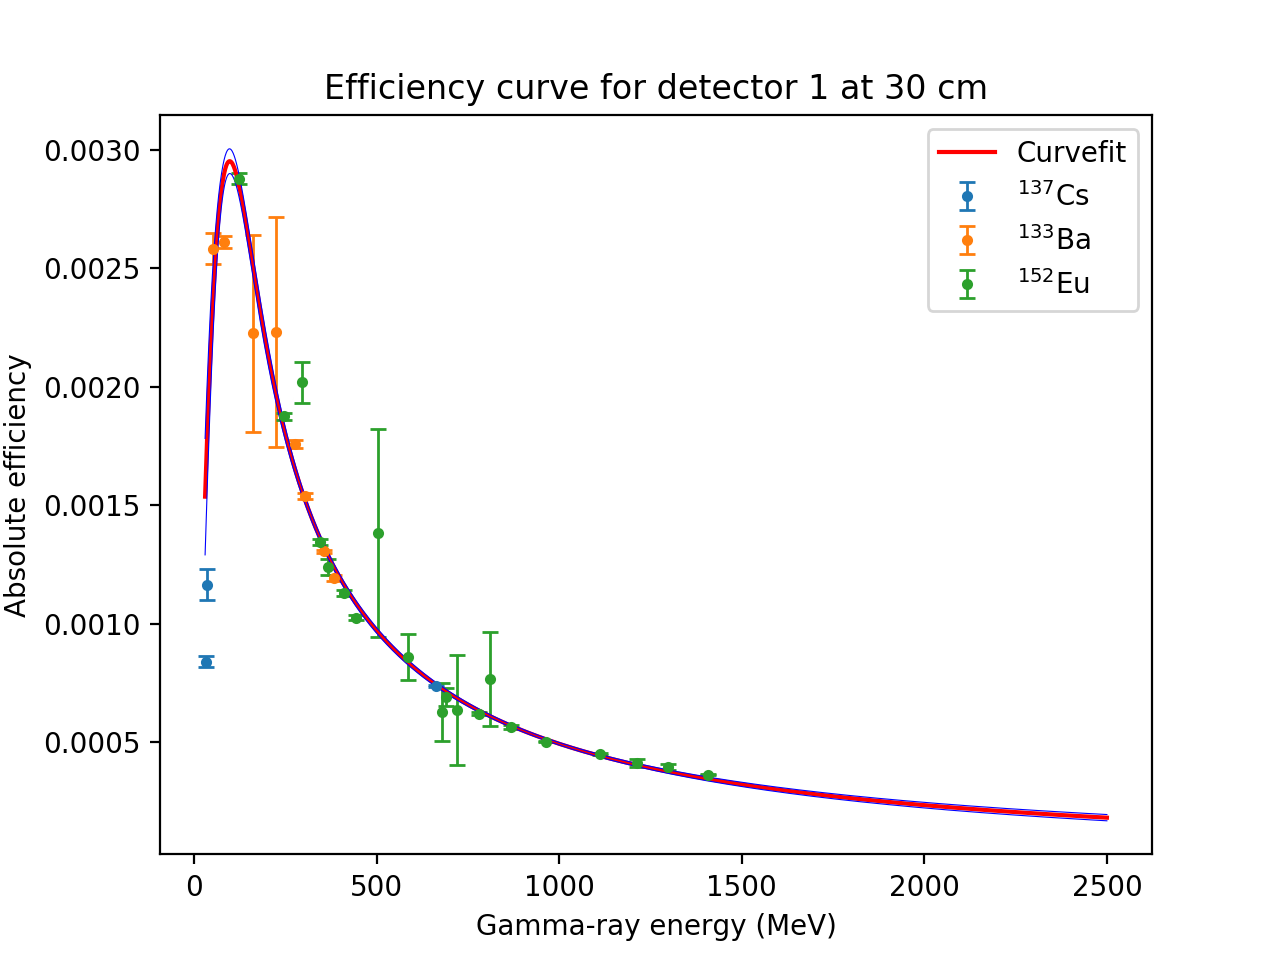
\includegraphics[width=12cm]{Experiment/new_det1_numb30cm.png} }}%
    
    \subfloat{{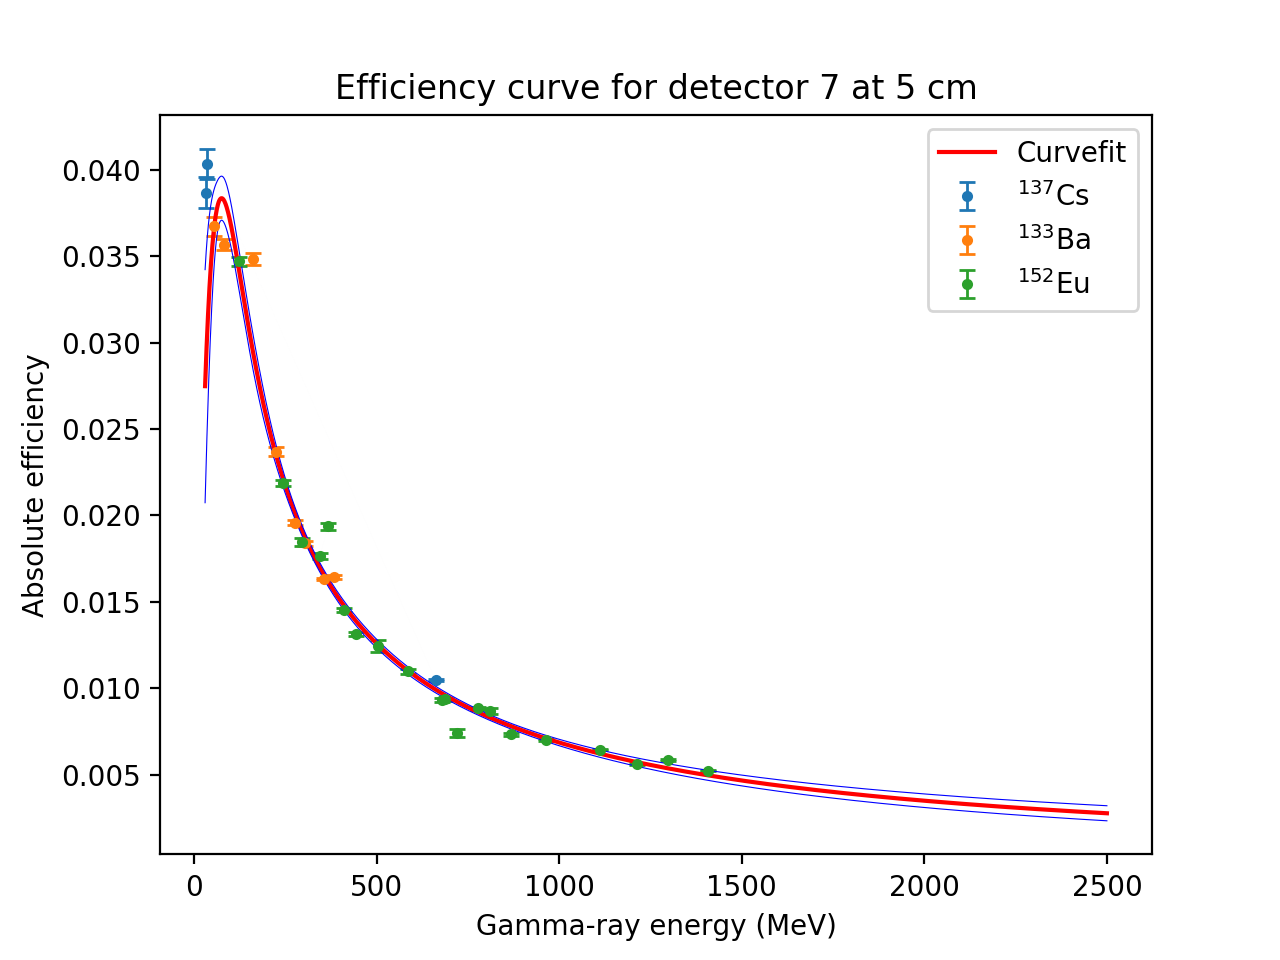
\includegraphics[width=12cm]{Experiment/new_det7_numb5cm.png} }}%
    \caption{Two examples of efficiency curves. \textbf{top}: The efficiency curve of detector 1 at 30 cm which is located in cave 4C. \textbf{bottom:} The efficiency curve of detector 7 at 5 cm is located in a separate room and had led shielding. }%
    \label{fig:efficiency_curves}%
\end{figure}


\begin{figure}%
    \centering
    \subfloat{{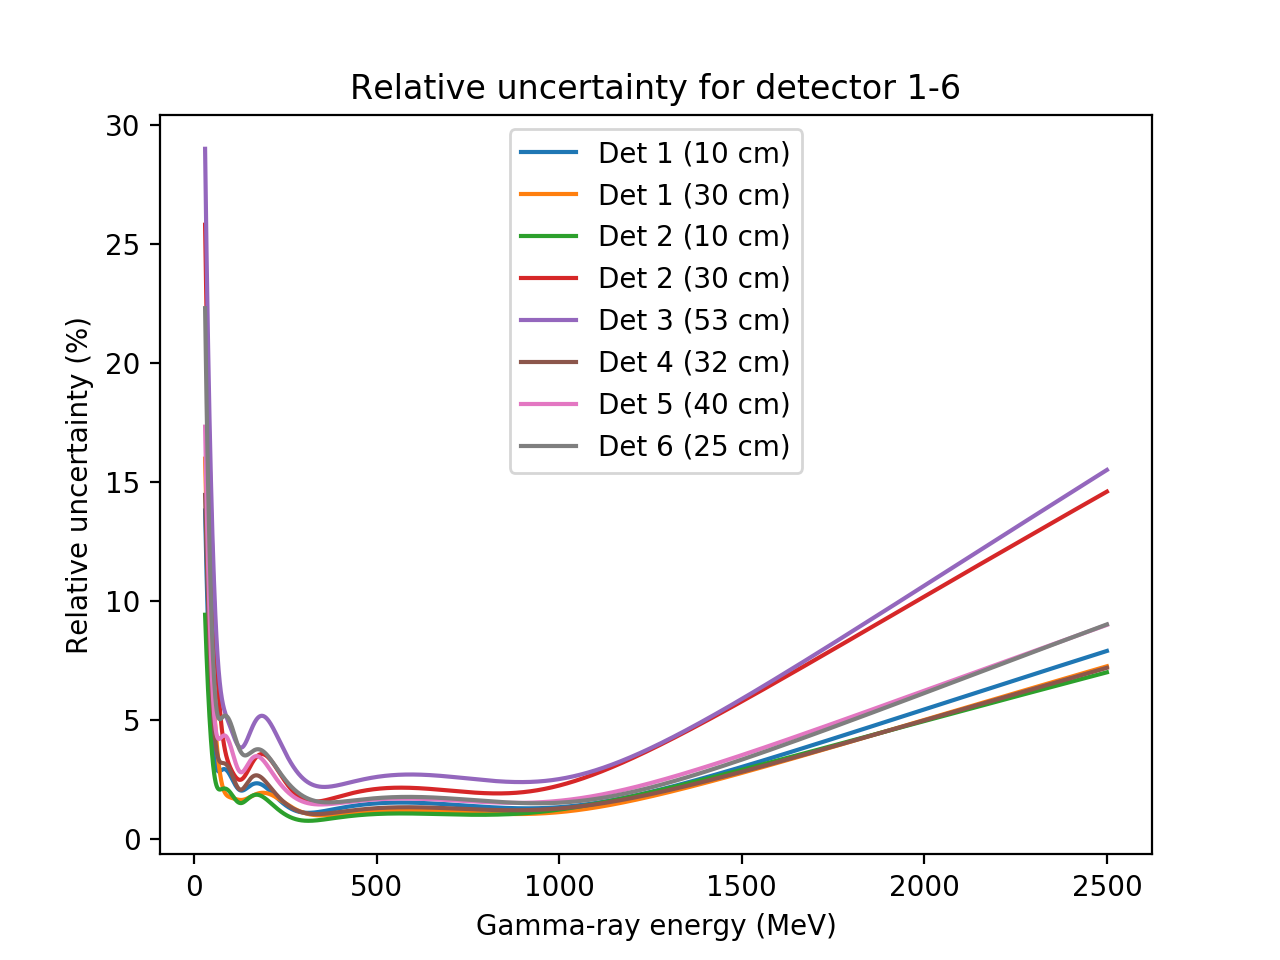
\includegraphics[width=12cm]{Experiment/Det1-6_rel_unc.png} }}%
    
    \subfloat{{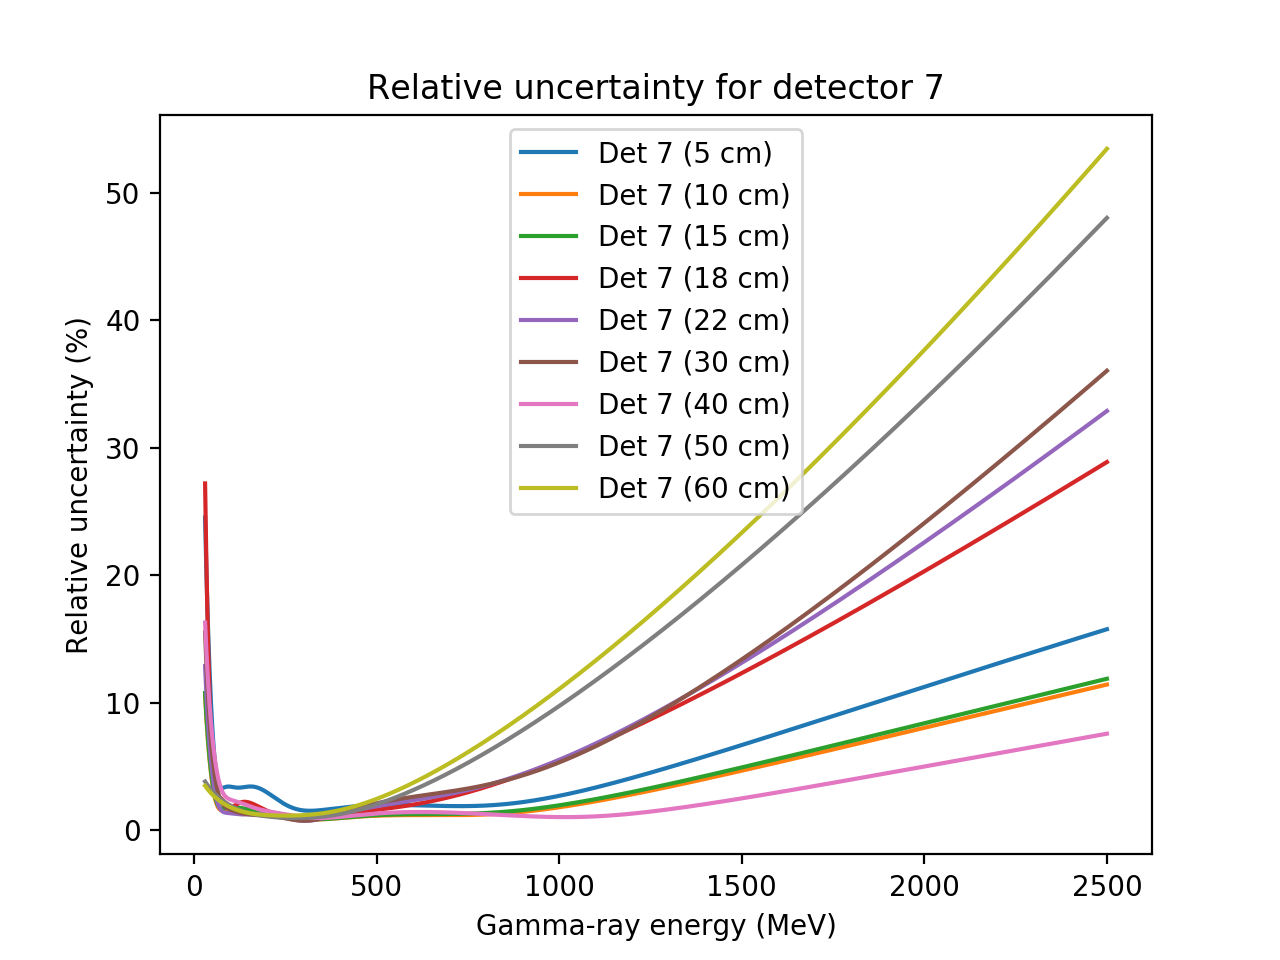
\includegraphics[width=12cm]{Experiment/rel_unc_room131.png} }}%
    \caption{The relative uncertainty in efficiency for each detector. \textbf{Left:} Relative uncertainty for detectors 1-6 (p-type IDM ORTEC). \textbf{Right:} Relative uncertainty for detector 7 (n-type ORTEC GMX).  }%
    \label{fig:rel_uncertainty_efficiency}%
\end{figure}




%\subsubsection{}

%The detectors were calibrated for efficiency,  peak shape and gamma-ray energy in the Gammaray-spectroscopy analyzation program Fitzpeaks. The calibration point sources $^{137}$Cs ($t_{1/2}=30.08$ years\cite{Browne2007}), $^{133}$Ba ($t_{1/2}=10.551$ years\cite{Khazov2011}) and $^{152}$Eu ($t_{1/2}=13.517$ years\cite{Martin2013}) were used with the gamma-lines listed in table \ref{table:calibration_gammas}. The calibration was done at various distances from the detector surface. The point sources can can be seen on figure \ref{fig:calsources}. The energy and peakshape calibration was done in FitzPeakz which is described in section \ref{subsec:fitz_calibration}. The efficiency calibration is described in section \ref{sec:efficiency_calibration}. \\ 




\section{The irradiation} \label{sec:experiment}
The irradiation of the target stack took place on February 26th 2019, and the activated foils were counted on high purity germanium detectors for a total of 4 weeks after end of beam. \textcolor{red}{In addition to this experiment, two other experiments took place, irradiating strontium with deuterons and a deuteron breakup experiment}. The target stack was subject to a 33 MeV incident deuteron beam, which can be seen in figure \ref{fig:experiment_illustration}. The beamintegrator measured the beamcurrent on the first foil to be 128.5 nA.     \\

%The main motivation of this experiment was to measure production cross sections of the products produced after irradiation of a stack of thin iridium foils along with thin monitor foils nickel, copper and iron foils, with a 33 MeV incident deuteron beam, as shown in figure \ref{fig:experiment_illustration}. 
\begin{figure}
    \centering
    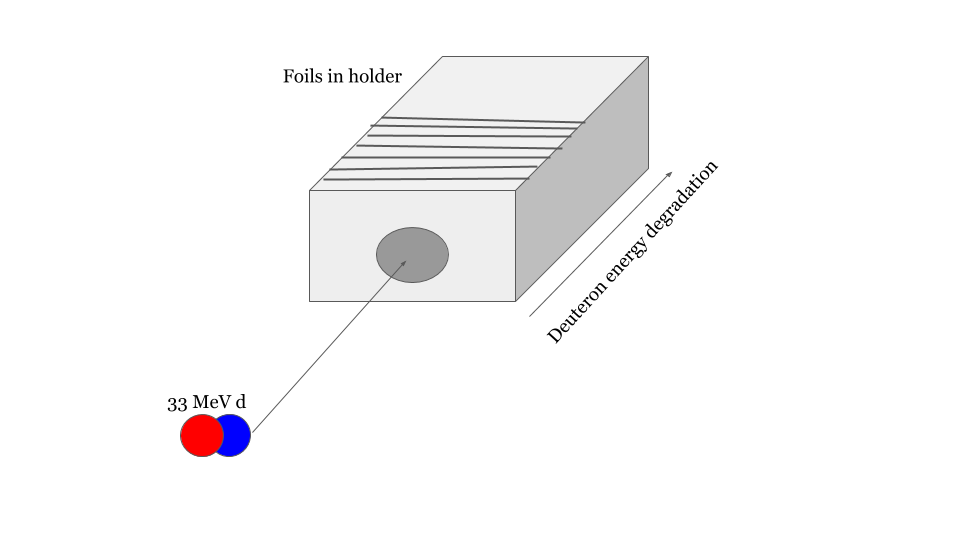
\includegraphics[width=0.7\textwidth]{Experiment/Illustration_beamOnTarget.png}
    \caption{The fundamental idea of the experiment where a stack of targets are placed in a target holder, and irradiated with accelerated 33 MeV deuterons. As the energy degrades through the beam stack, it is possible to have multiple cross section measurements at different energies.}
    \label{fig:experiment_illustration}
\end{figure}

\noindent 
\begin{comment}
FIND A SOURCE WHICH WRITES MORE!
The stacked target activation method is a technique where multiple cross sections can be measured using one single incident beam on a stack of thin targets. The cross sections are estimated by the activation of each product in each foil. 
The stacked-target method originates from Graves et. al. irradiating a stack of thin iron, copper and aluminum foils with a 35-90 MeV protons beam \cite{Graves2016}. The method yields reaction cross section measurements at multiple energies for products which are observed in the foils with gamma-ray spectroscopy, as a stack of thin targets are exposed to a single incident charged particle beam which is degraded in the foils. Recent measurements conducted at Lawrence Berkeley's 88-Inch cyclotron have taken place over the past years using protons for reactions on iron, copper and titanium from threshold to 55 MeV  \textcolor{red}{cite Fe-paper}%\footnote{https://www.researchgate.net/publication/336796889_Proton-induced_reactions_on_Fe_Cu_Ti_from_threshold_to_55_MeV}
and for reactions on niobium using 40-90 MeV protons\cite{Voyles2018c}. The induced activities in the foils can be measured and transferred into cross sections. For a thin foil, the beam degradation is small in comparison to thick targets, and the uncertainty in beam energy is thus small. In addition, the use of thin foils with a thickness of a few $\mu$m allows for low activation in each foil, which reduces dead time of the detector, along with lower dose to workers which is advantageous for isotope production and cross section measurement\cite{Qaim2017c}. \\

\noindent 
 The stack consisted of natural iridium (99.9\%), natural nickel (..), natural copper (..) and natural iron (..) from Goodfellow Corporation, Corapolis, PA 15108, USA. Deuteron-induced products from iridium was the main motivation behind this experiment, primarily because of the potential medically valuable $^{193m}$Pt-isomer, and the contribution of nuclear reaction data of the natural iridium (d,x) reactions. For the latter three targets, the well-characterized cross section reactions $^\text{nat}$Fe(d,x)$^{56}$Co, $^\text{nat}$Ni(d,x)$^{61}$Cu$^{56,58}$Co and $^\text{nat}$Cu(d,x)$^{62,63,65}$Zn from the IAEA monitor database\cite{Hermanne2018a} were used to estimate the weighted average beam current throughout each compartment of foils. In addition, cross sections from deuteron induced products on these targets is a contribution to nuclear reaction data. The stack consisted of 10 nickel, 10 iridium, 10 copper and 3 iron foils, in which the order can be seen in table \ref{table:foil_characterization}. In addition to the target foils, two 316 stainless steel foils were placed in the front and the back of the stack, and a 6061 aluminum alloy which works as a proton degrader along with a nickel neutron monitor foil \textcolor{red}{to stop broken up deuterons (protons+neutrons)}. Since the number of targets in the stack worked as a beam degrader, the need of additional energy degraders in the stack was not necessary. The stainless steel worked as a beam profile monitor, as the activated foils could be used to develop Gafcromic films (radiochromic films) which contains a dye changing color when exposed to ionizing radiation (wiki, radiochromic) which can be used to build confidence in the spatial beam profile in the front and in the back of the stack. The full order of the stack can be viewed in table \ref{table:foil_characterization}. The stack design was decided upon the energy-degradation  of the stack with a package called NPAT's (nuclear ....) Ziegler simulation (decribed in section \ref{sec:beamcurrent}), which bases the stopping power on Anderson \& Ziegler stoppingpower formalism (\textcolor{red}{Cite anderson\& Ziegler and John}), so that the beam was not stopped in the target stack and all the foils were activated.  
\end{comment}

%From equation \ref{eq:activity_eob}, the cross section as a function of energy is 

%\begin{equation} \label{eq:experimental_CS}
%    \sigma(E)=\frac{A_0}{N_T \Phi (1-e^{-\lambda \Delta t_\text{irr}})}
%\end{equation}
 
%where E is the average energy across the foil (MeV), $A_0$ is the end of beam activity (Bq), $N_T$ is the number of target nuclei, $\Phi$ is the beam current (nA), $\lambda$ is the decay constant of the nucleus ($s^{-1}$) and $\Delta t_\text{irr}$ is the irradiation length (s). 

%Equation \ref{eq:cross_section_equation} is the equation which is used in the calculation of the cross sections. In order to calculate the cross section of a product, end of beam activity, number of target nuclei and beam current must be found, where for the end of beam activity, the detector efficiency need to be estimated. The number of target nuclei was estimated through characterization of the foils. $A_0$ was estimated using equation \ref{eq:Final_Expression_A0}, which depends on the efficiency calibration of the detectors as a function of gamma-ray energy, the number of counts registered and the intensity of the gamma-rays emitted by the source, the decay constant of the source and the delay time. Some of the nickel, copper and iron deuteron-induced cross section are well-established, and can  be used to determine the beam current throughout the stack. 



%The end of beam activity goes into the equation, which is given in equation \ref{eq:Final_Expression_A}. The activity from spectra measured at different delay times after end of beam can be found, with respect to number of counts, efficiency of detector, intensity of gamma-rays, the decay constant of the nucleus $\lambda$ and the counting time $\Delta t_c$. As we know that radioactive decay curves follows equation \ref{eq:ndecay_chains}, and dependent on how many step the decaychain consists of, the end of beam activity can be estimated by extrapolating backwards in time with a curve fit. \\

%\noindent 


\textcolor{red}{
\noindent 
When a target is irradiated, the activity of the product nucleus will increase until secular equilibrium is achieved, which is when the product rate and decay rate are constant. Hence it is not necessary to irradiate a target for more than 2-3 half lives.\\. WHY WAS THE STACK IRRADIATED FOR ONE HOUR???}

\subsubsection{The tuning the beam}
Before irradiation, the deuteron beam was tuned to be ca. 1 cm in diameter. In addition, the experiments taking place simultaneously demanded a precise position of the beamspot since the target size was on the order of the same order of the beamspot. The beam spot was first visualized using a ca. 2.5 cm thick borosilicate glass, painted with a mixture of phosphor powder and vacuum grease (so that the paint does not evaporate as the tube was pumped down to vacuum). When ionizing radiation strikes the phosphor, the phosphor is excited and emits light in the de-excitation, called phosphorescence.  The glass was placed on the end of the beam tube. With a camera placed in cave 0, from the control room, the beam spot could be visualized, and could be steered to be centered and ca. 1 cm in diameter. The beamspot can be visalized in figure \ref{fig:tuning_phosphor+camera} (left), and the borosilicate glass placed on the end of the beam tube can be seen in figure \ref{fig:tuning_phosphor+camera} (right). Secondly, the beam had to be constant over the target stack, \textcolor{red}{i.e. not diverge or converge}. Gafchromic films were placed in the front and the back of the target holder, separated by the spring. The films were exposed for a brief second, and the blue spot on the developed film was evaluated. This was done until the beamspot was good both in the front and in the back of the stack. The Gafchromic films after direct exposure can be seen in figure \ref{fig:tuning_gafchromic} in the target holder.  \\

\begin{figure}%
    \centering
    \subfloat[]{{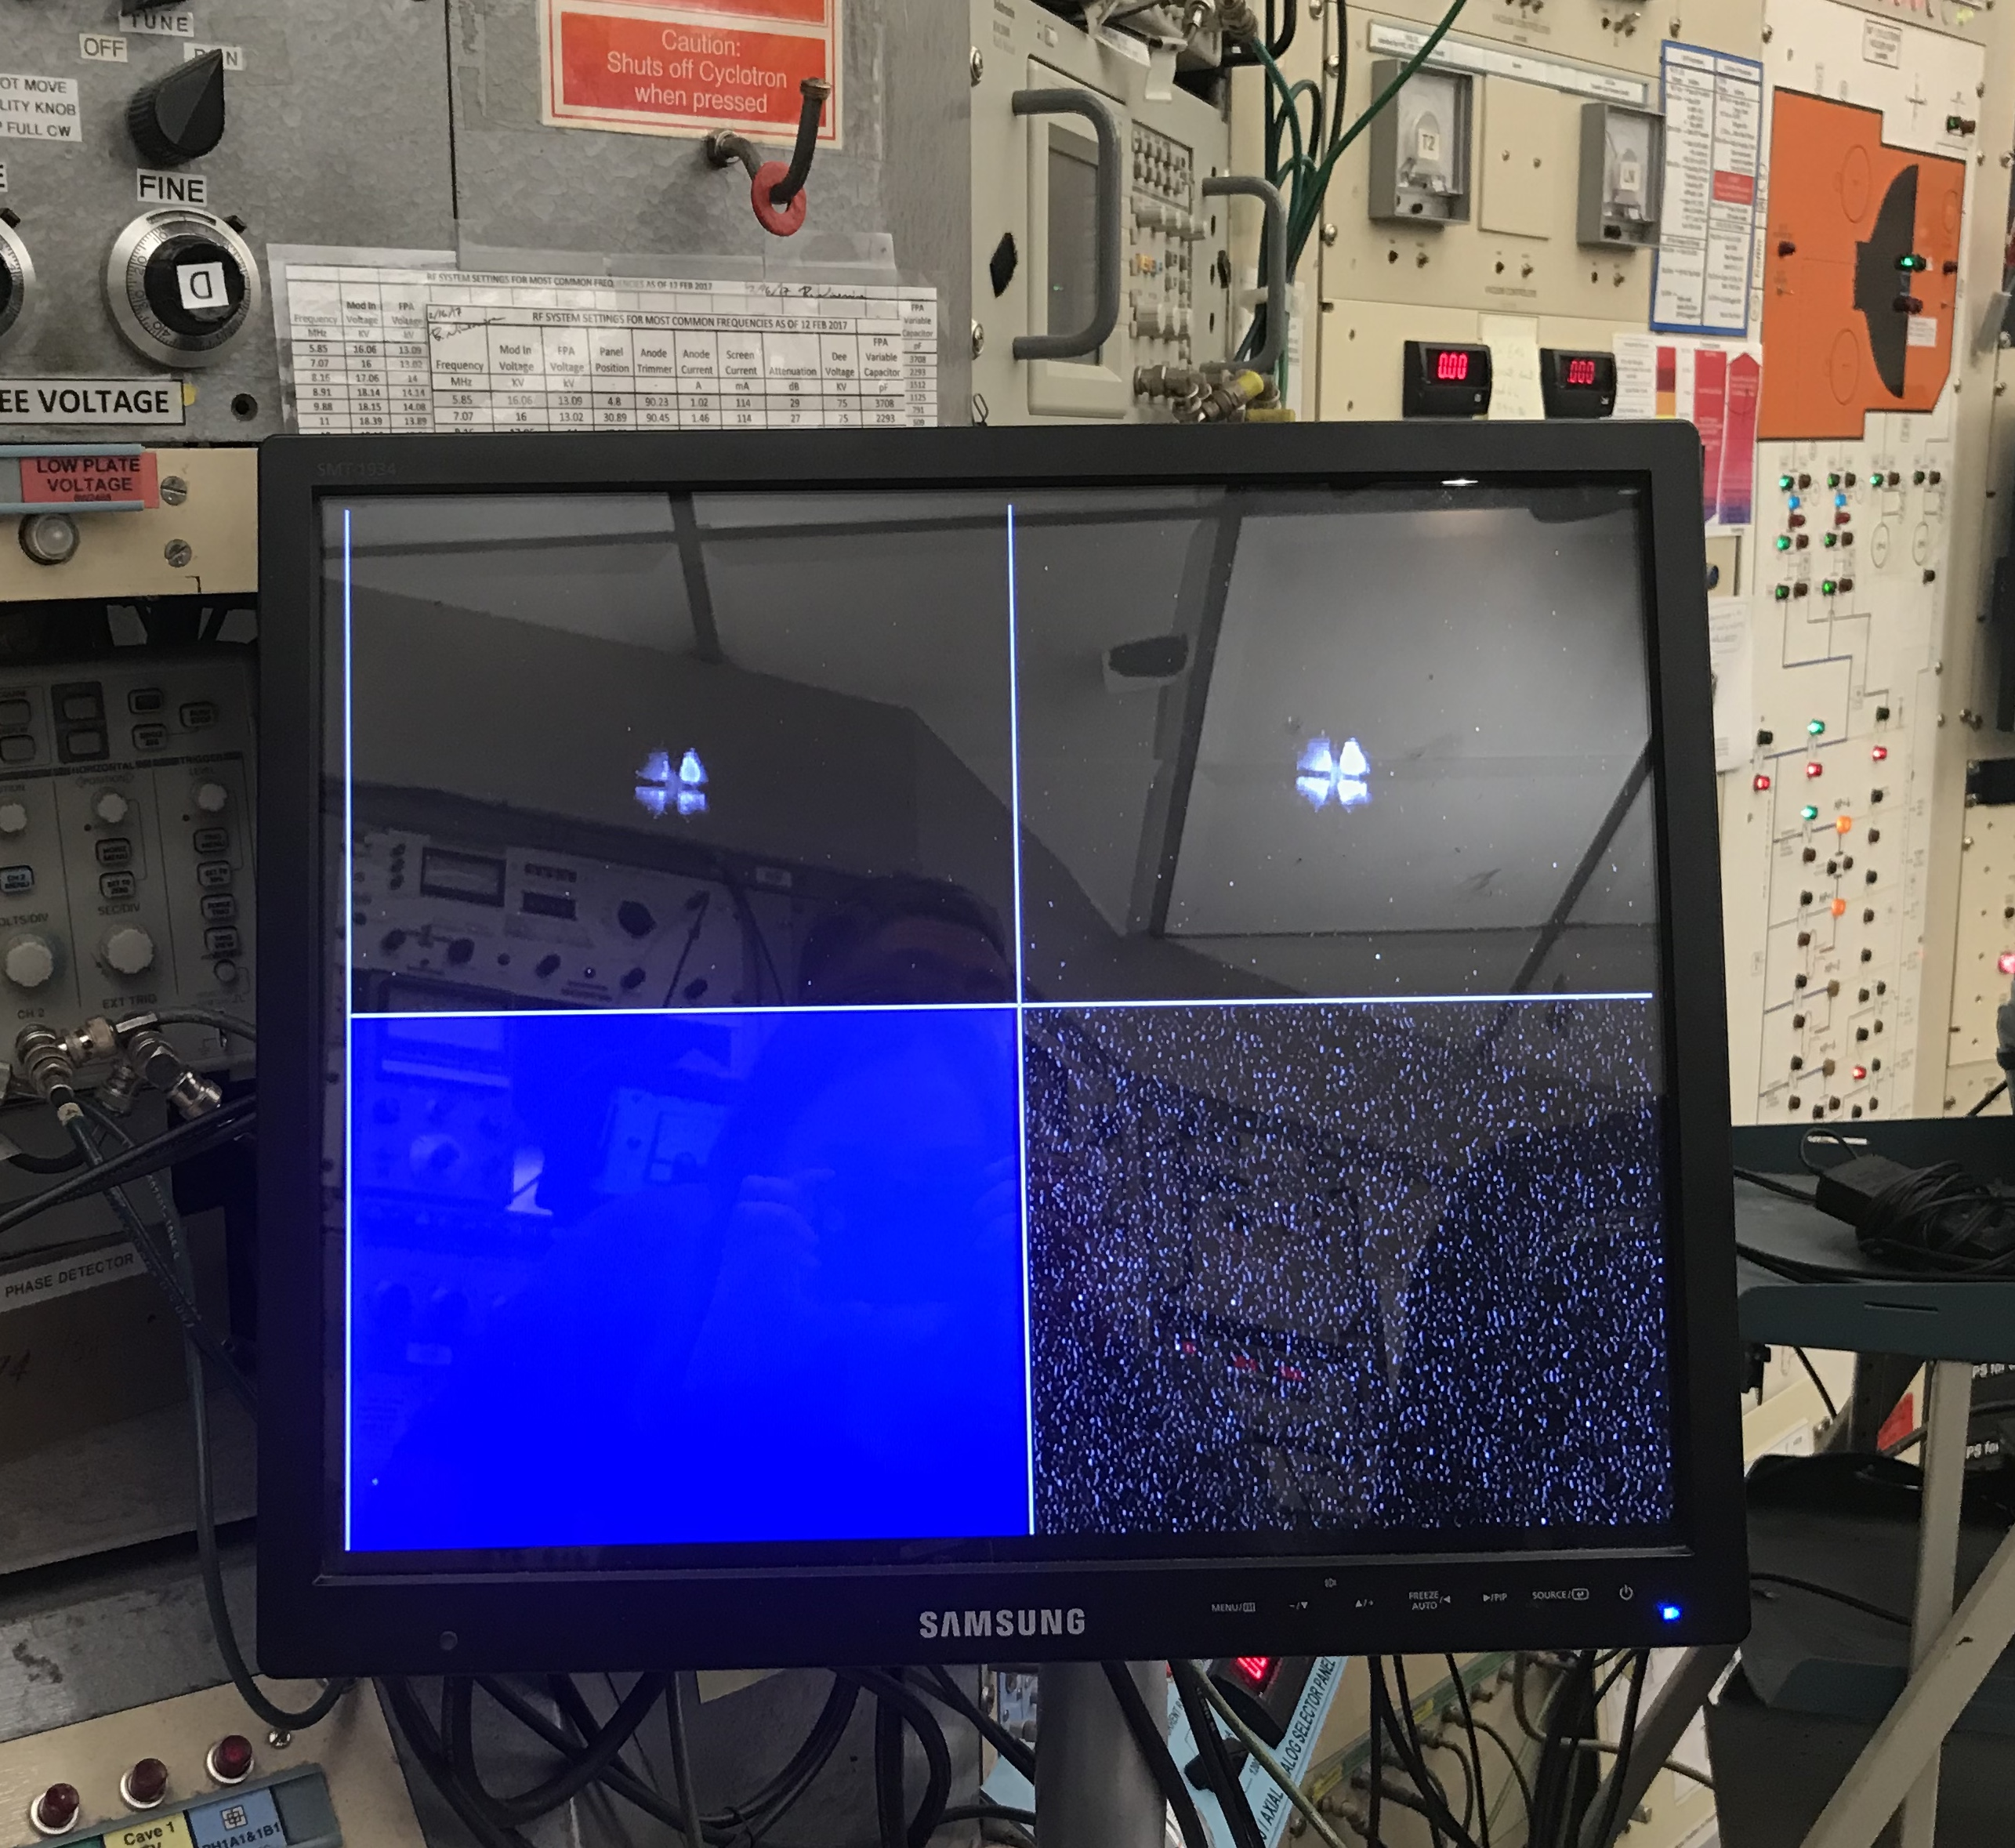
\includegraphics[width=6.6cm]{Experiment/beamspot_visualization.jpg} }}%
    \subfloat[]{{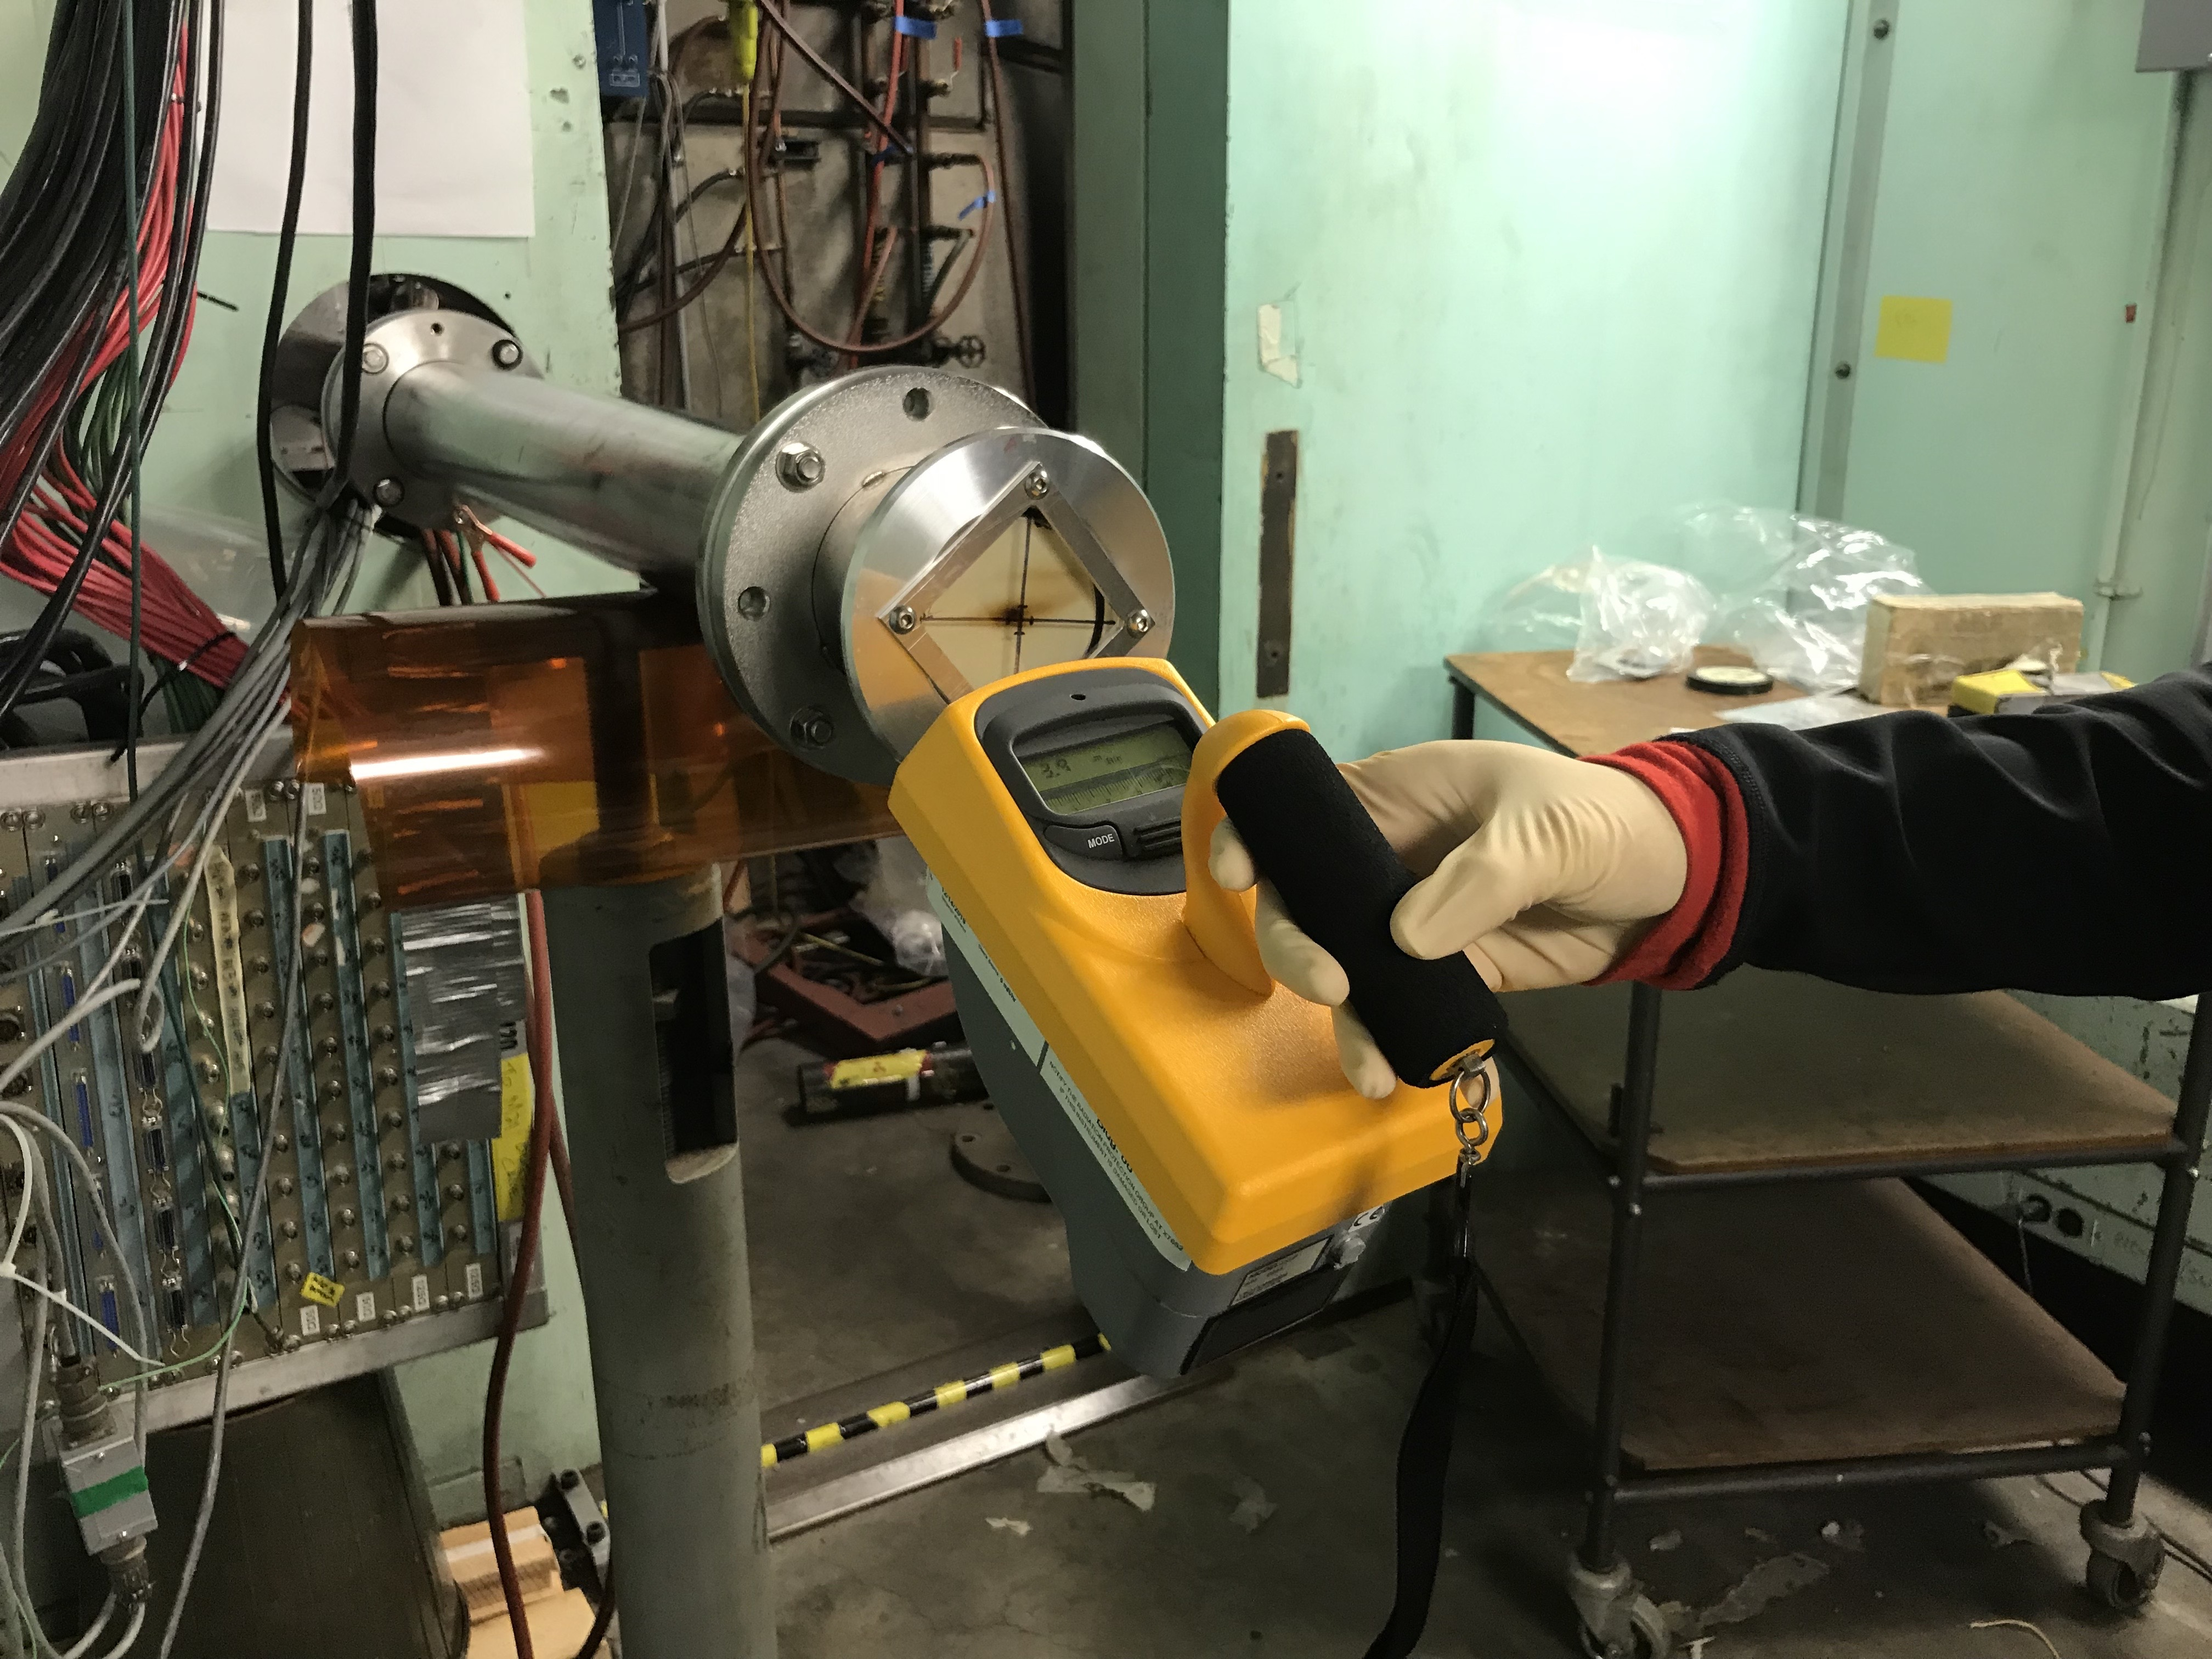
\includegraphics[width=6.6cm]{Experiment/phosphor_plate.JPG} }}%
    \caption{The figure shows the beamspot which could be visualized from the control room, and the borosilicate glass placed on the end of the beam tube. The dose present after the beam was on was always measured. }%
    \label{fig:tuning_phosphor+camera}%
\end{figure}

\begin{figure}
    \centering
    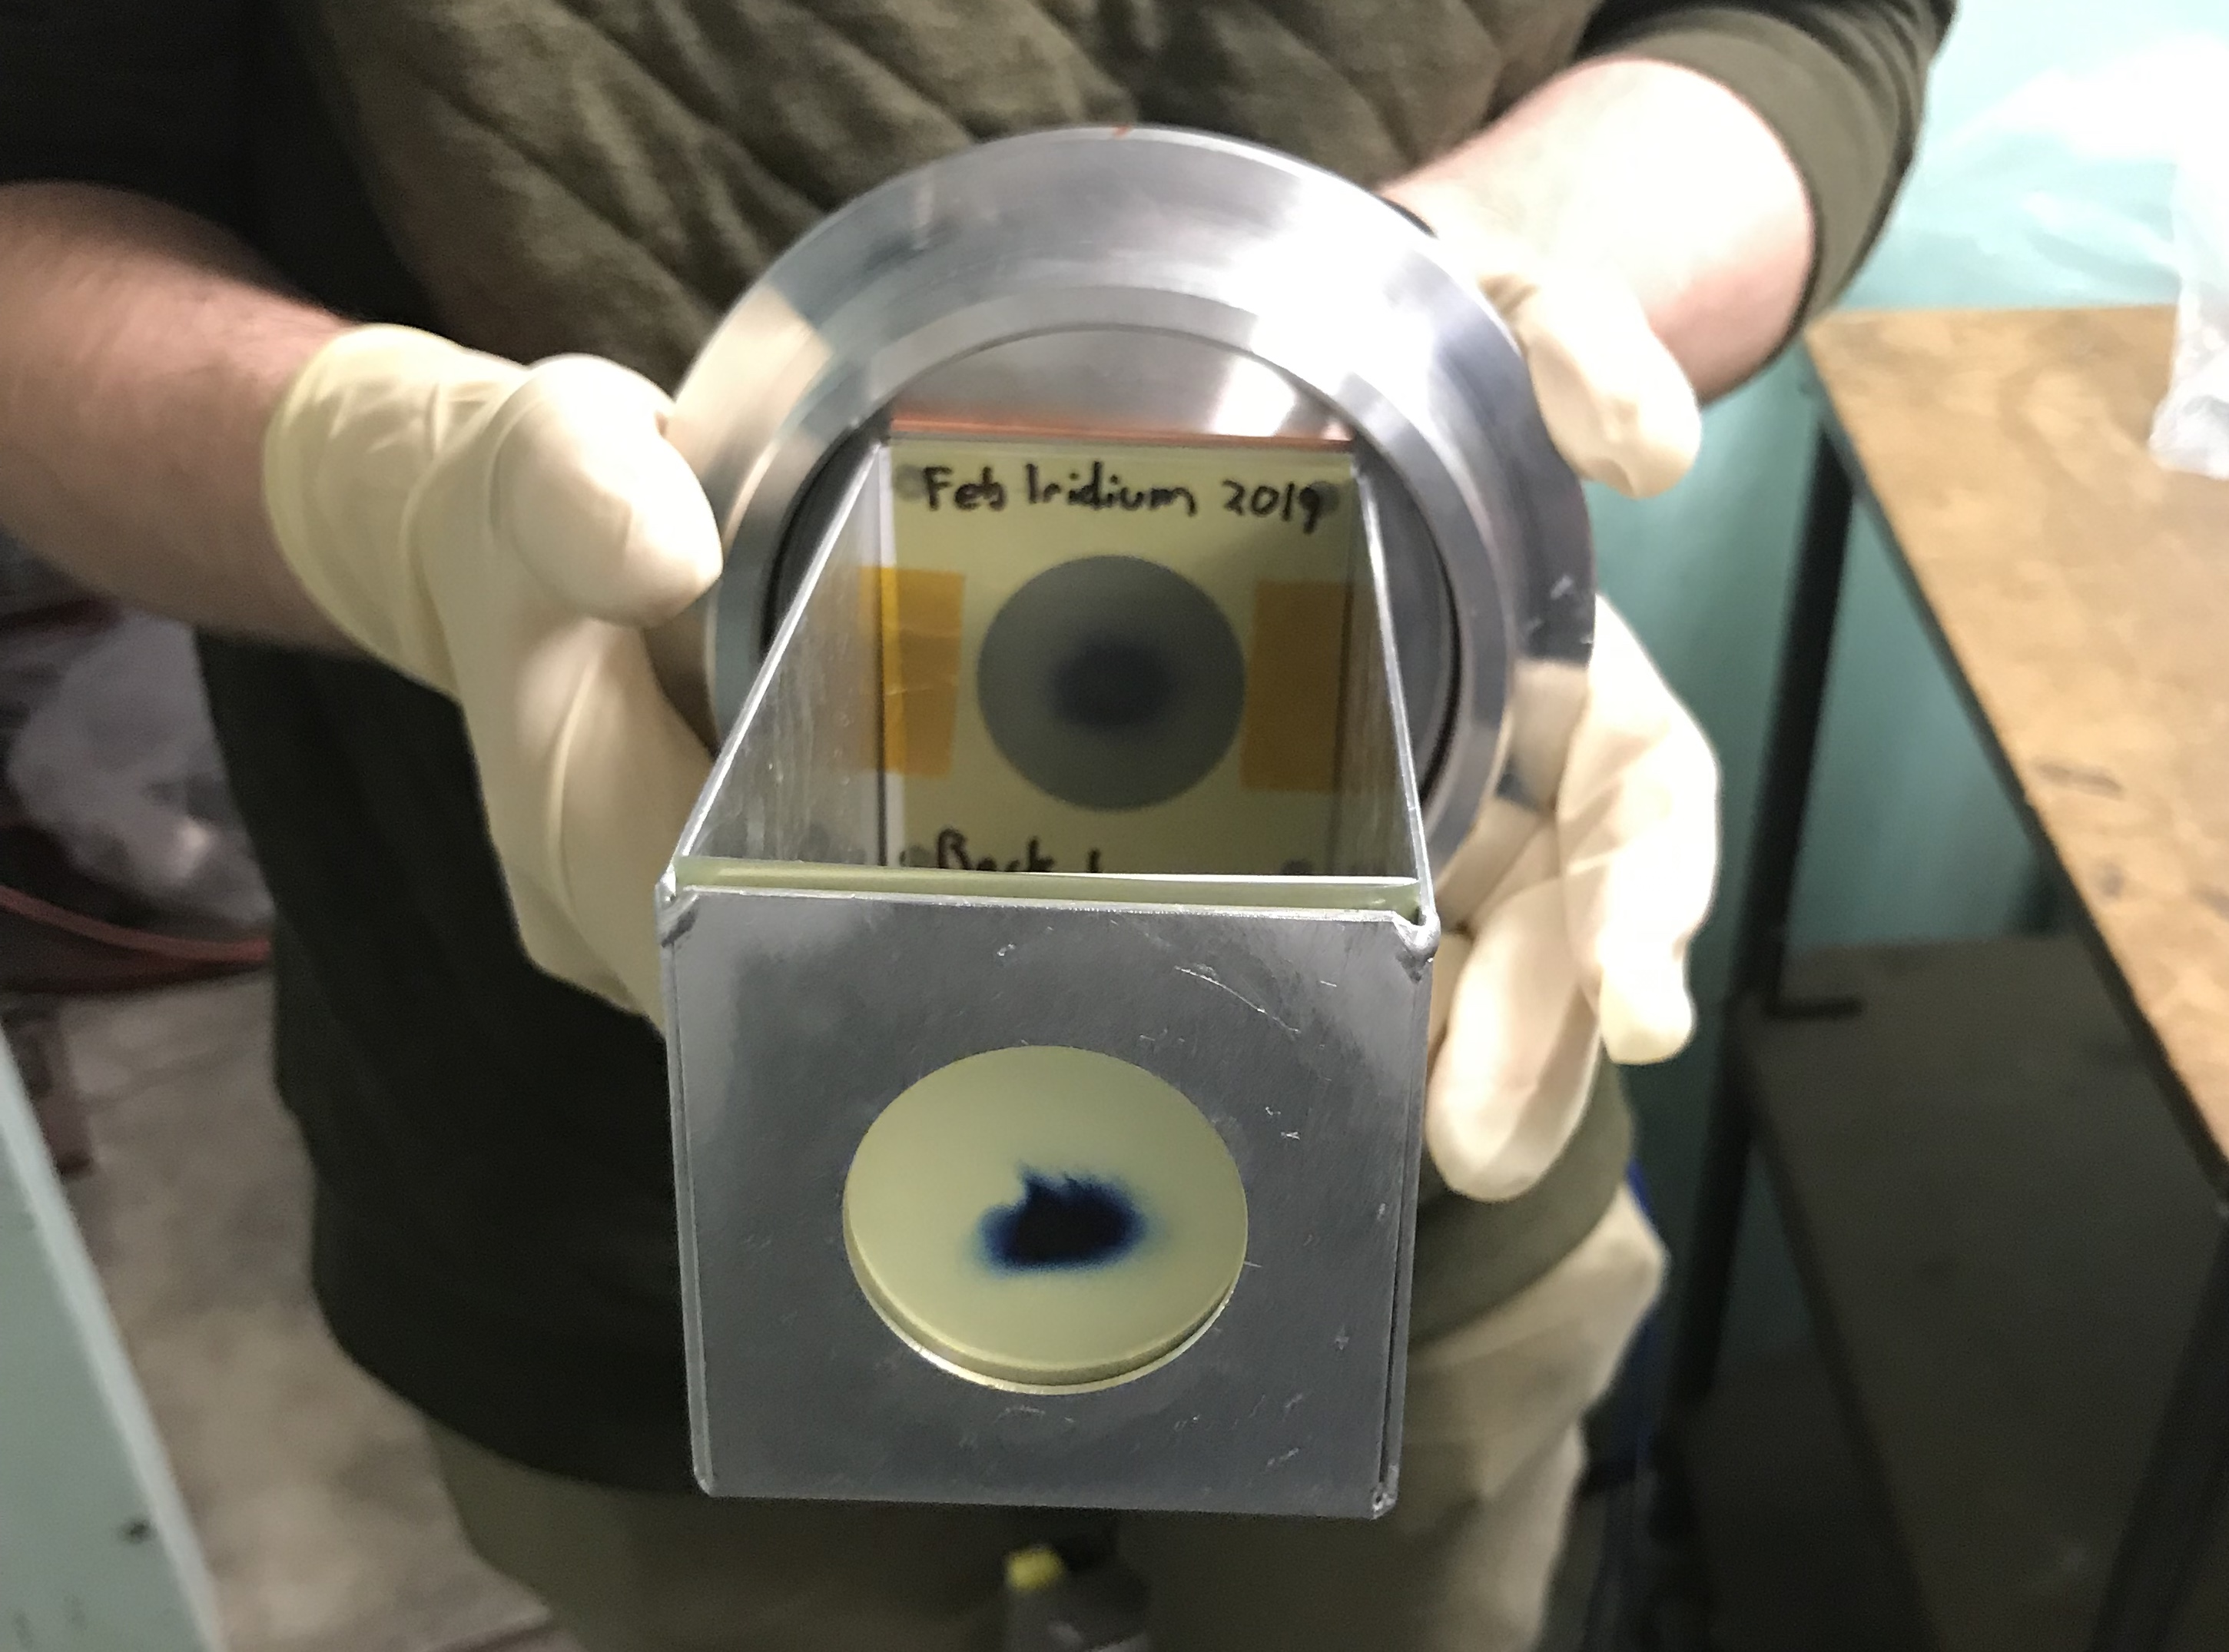
\includegraphics[width=0.7\textwidth]{Experiment/gafchromic_tune.jpg}
    \caption{The gafchromic films were exposed for a brief second }
    \label{fig:tuning_gafchromic}
\end{figure}

\noindent
The beam efficiency transmission was calculated by measuring the the current at the Faraday cup right after the cyclotron vault (BS-02) and right before cave 0 (FC-01). BS-02 was measured to be 420 nA and FC-01 was measured to be 285 nA. This gave beam efficiency of transmission of 67\%

%$$\frac{FC-01}{BS-02}=67\% $$


\subsubsection{Irradiation of the target stack} 
The irradiation lasted for one hour. The number of \textcolor{red}{charges collected??} was registered off the current integrator on the \textcolor{red}{electrically isolated beamline}, and registered evenly to ensure that the beamcurrent was more or less constant throughout the irradiation. After exactly one hour, the beam integrator read of $I\Delta t= 2314$ C, with full-scale amperes being $2\cdot10^{-7}$ A. The average beam current hitting the front of the stack was thus 

\begin{equation}
    \frac{2314\cdot 2\cdot10^{-7}}{3600 } = 128.5 \text{ nA}
\end{equation}

Before the beam was turned on, the beam tube had to be pumped down to a vacuum, to not attenuate the beam. The targetholder was placed in the end of the electrically isolated beam tube. Figure \ref{fig:targetstack} shows how the targetholder (left) was placed in the end of the beam line (right). About ten minutes after end of beam, cave 0 was opened, and the targets were sealed in plastic bags to avoid contamination. The iridium foils was counted from 15 minutes after end of beam on detector 7, and the other foils following up shortly after. All the foils were counted for ca. four weeks following end of beam on the various detectors, with short counts in the beginning to have good statistical data for the short-lived activities, and longer and longer counts as the shorter and medium-lived activities decayed out, to have good statistics. The counts were done as jobscripts in the beginning, so that the same foil was measured multiple times, and the gamma-lines were observed multiple times over short counts rather than one long count. The reason why the foils were counted multiple times was to reduce the statistical uncertainty, and in addition make sure that the products with similar gamma-lines but different half-lives were observed independently if possible. Since the detectors were calibrated at various distances, the deadtime of the foils right after end of beam could be reduced by increasing the distance from the detector, however, as high as  16-22\% deadtime was present, but reduced to less than 5\% within a cooling time of ca. 1 day after end of beam \textcolor{red}{double check, but on quick overview this seemed right}.
$^{193m}$Pt has one single weak gamma-line at 135.5 keV (0.11\%). In addition, it i located at the shoulder of $^{192}$Ir at 136.39 (0.199\%) \cite{ShamsuzzohaBasunia2017a, Baglin2012}. The half-life of $^{192}$Ir is long, and it was important to make sure that the two peaks were identified independently. 
Due to the relatively long half-life of $^{193m}$Pt, and the weak gamma-ray, it was made sure that the single gamma-line was observed within a few days after end of beam, when the counts were longer. 

%The foils were counted at the seven different high purity germanium detectors for the following 4 weeks after end of beam, first short counts to get as many observations as possible of the short-lived activities and longer and longer counts as the times since end of beam passed, so that the counting statistics for the longer lived activities were good. 
\noindent 


\begin{figure}%
    \centering
    \subfloat{{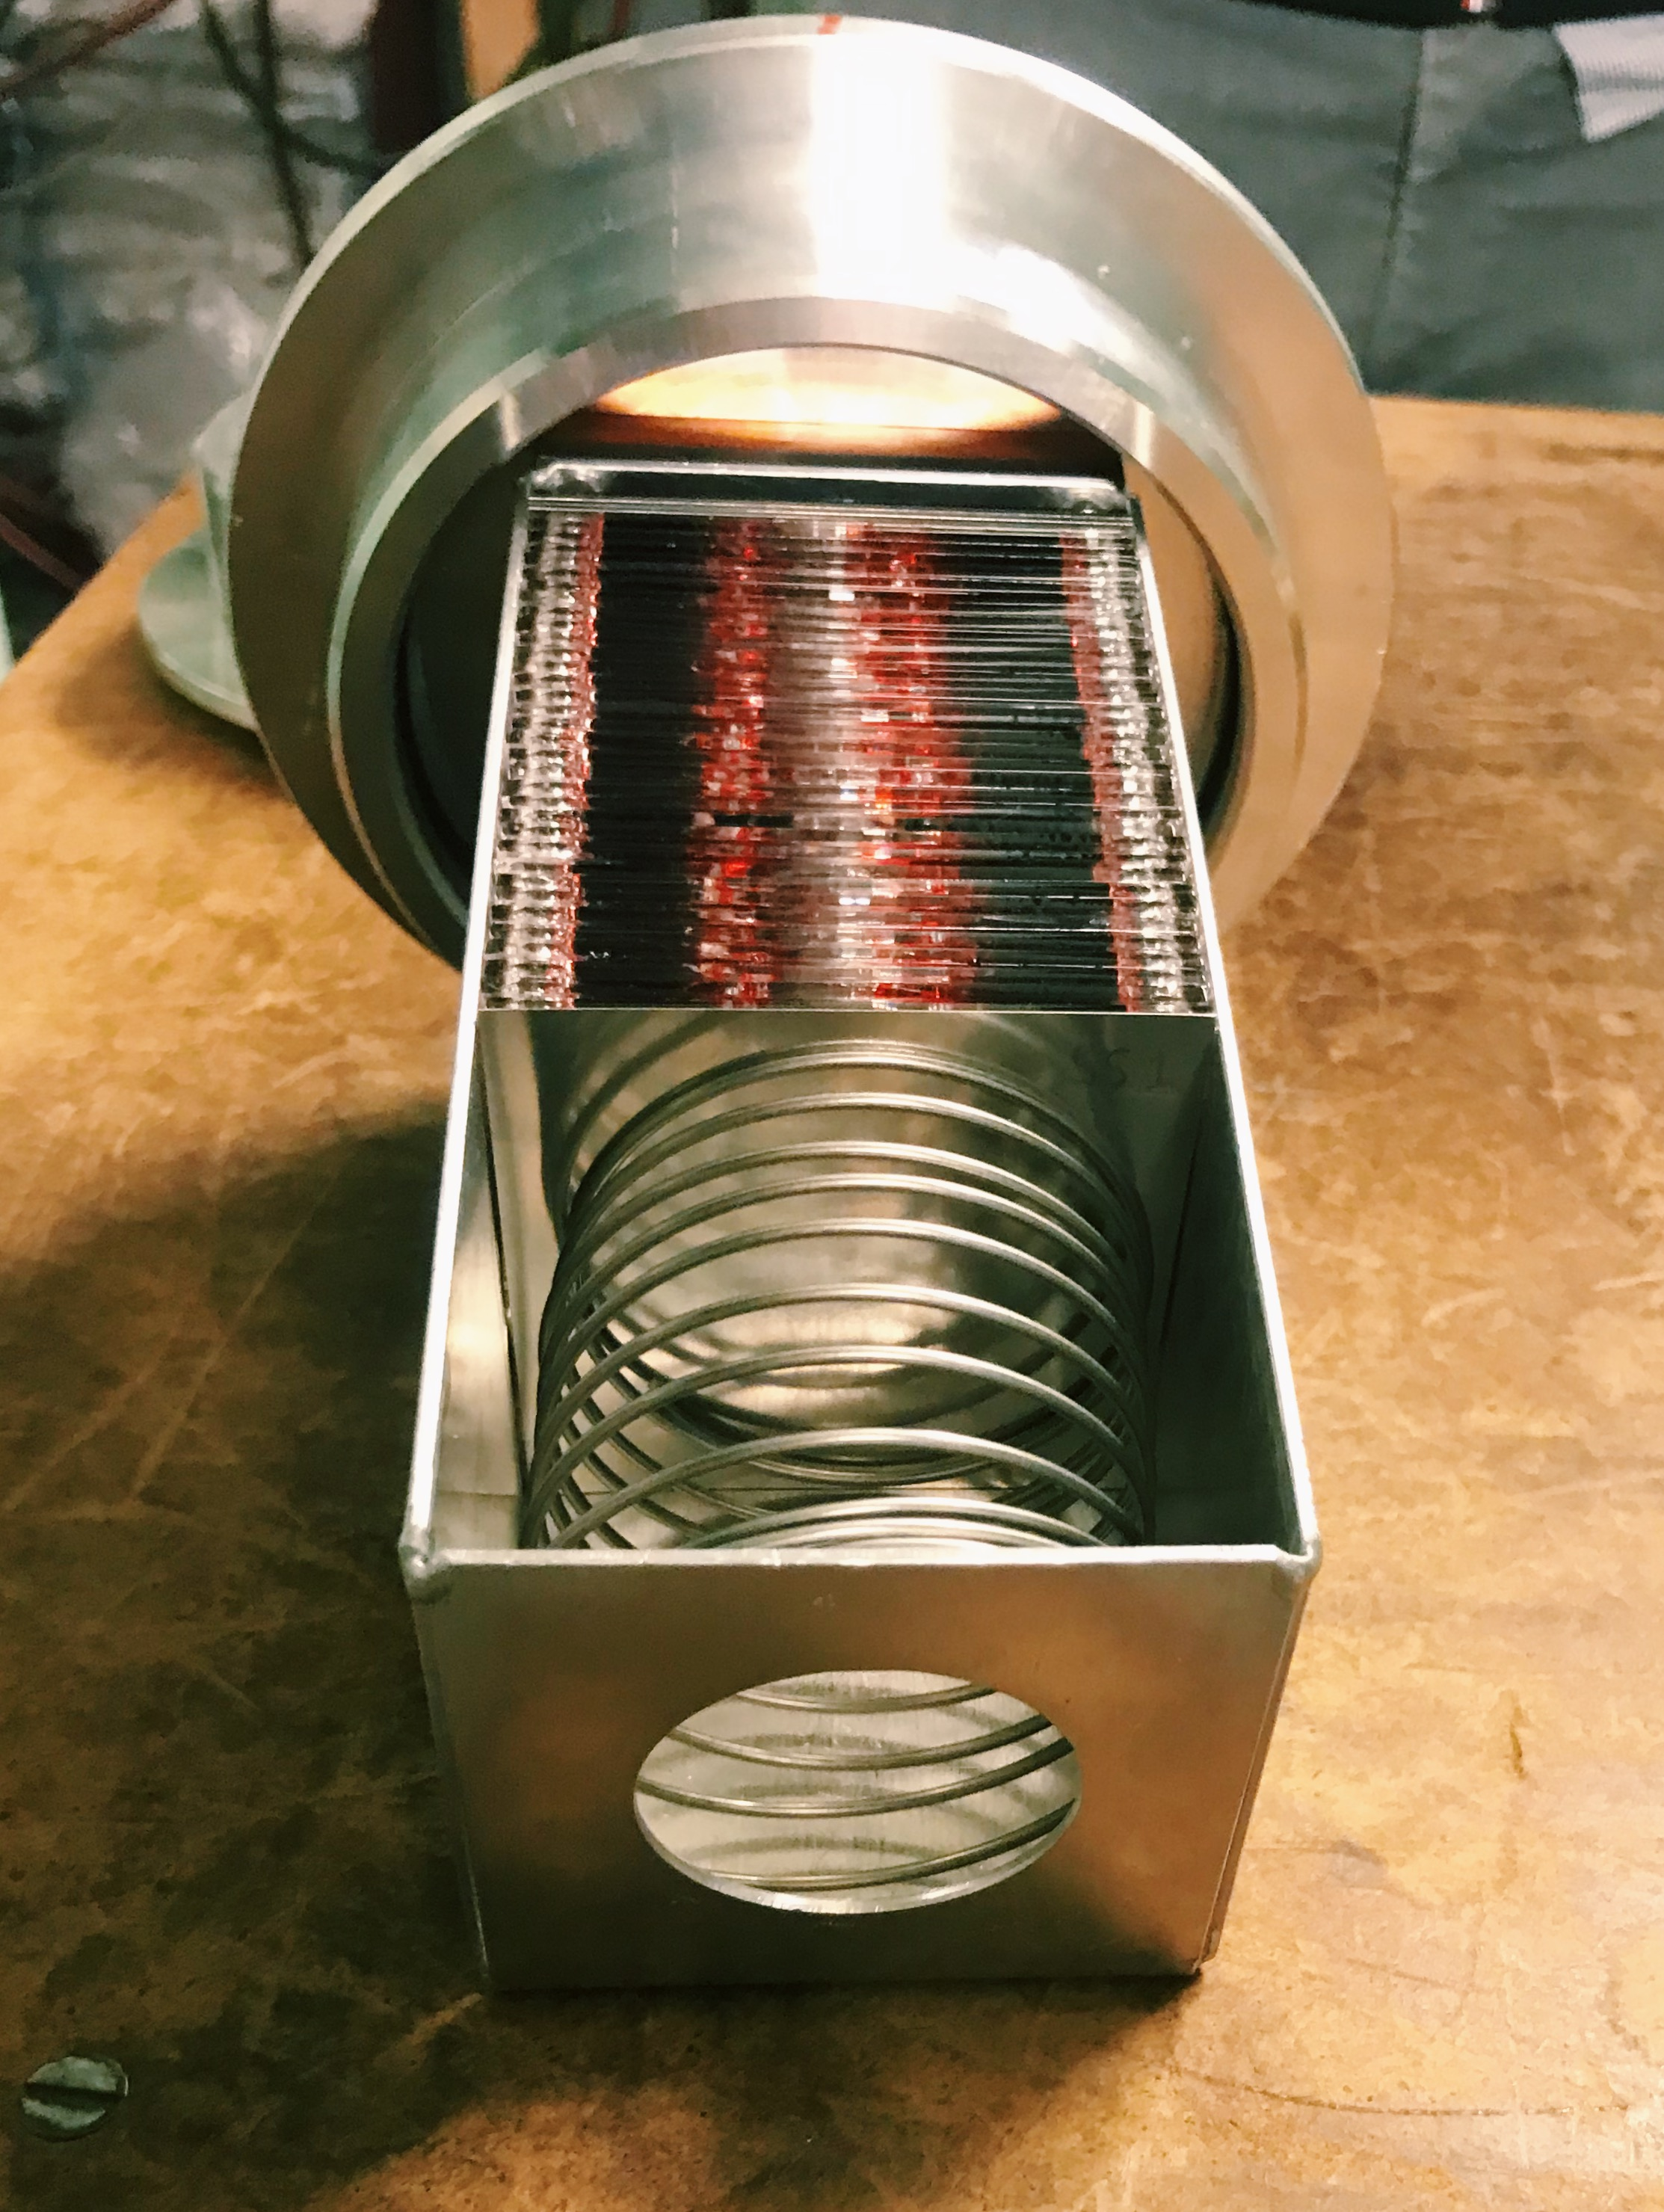
\includegraphics[width=6.6cm]{Experiment/stack.JPG} }}%
    \subfloat{{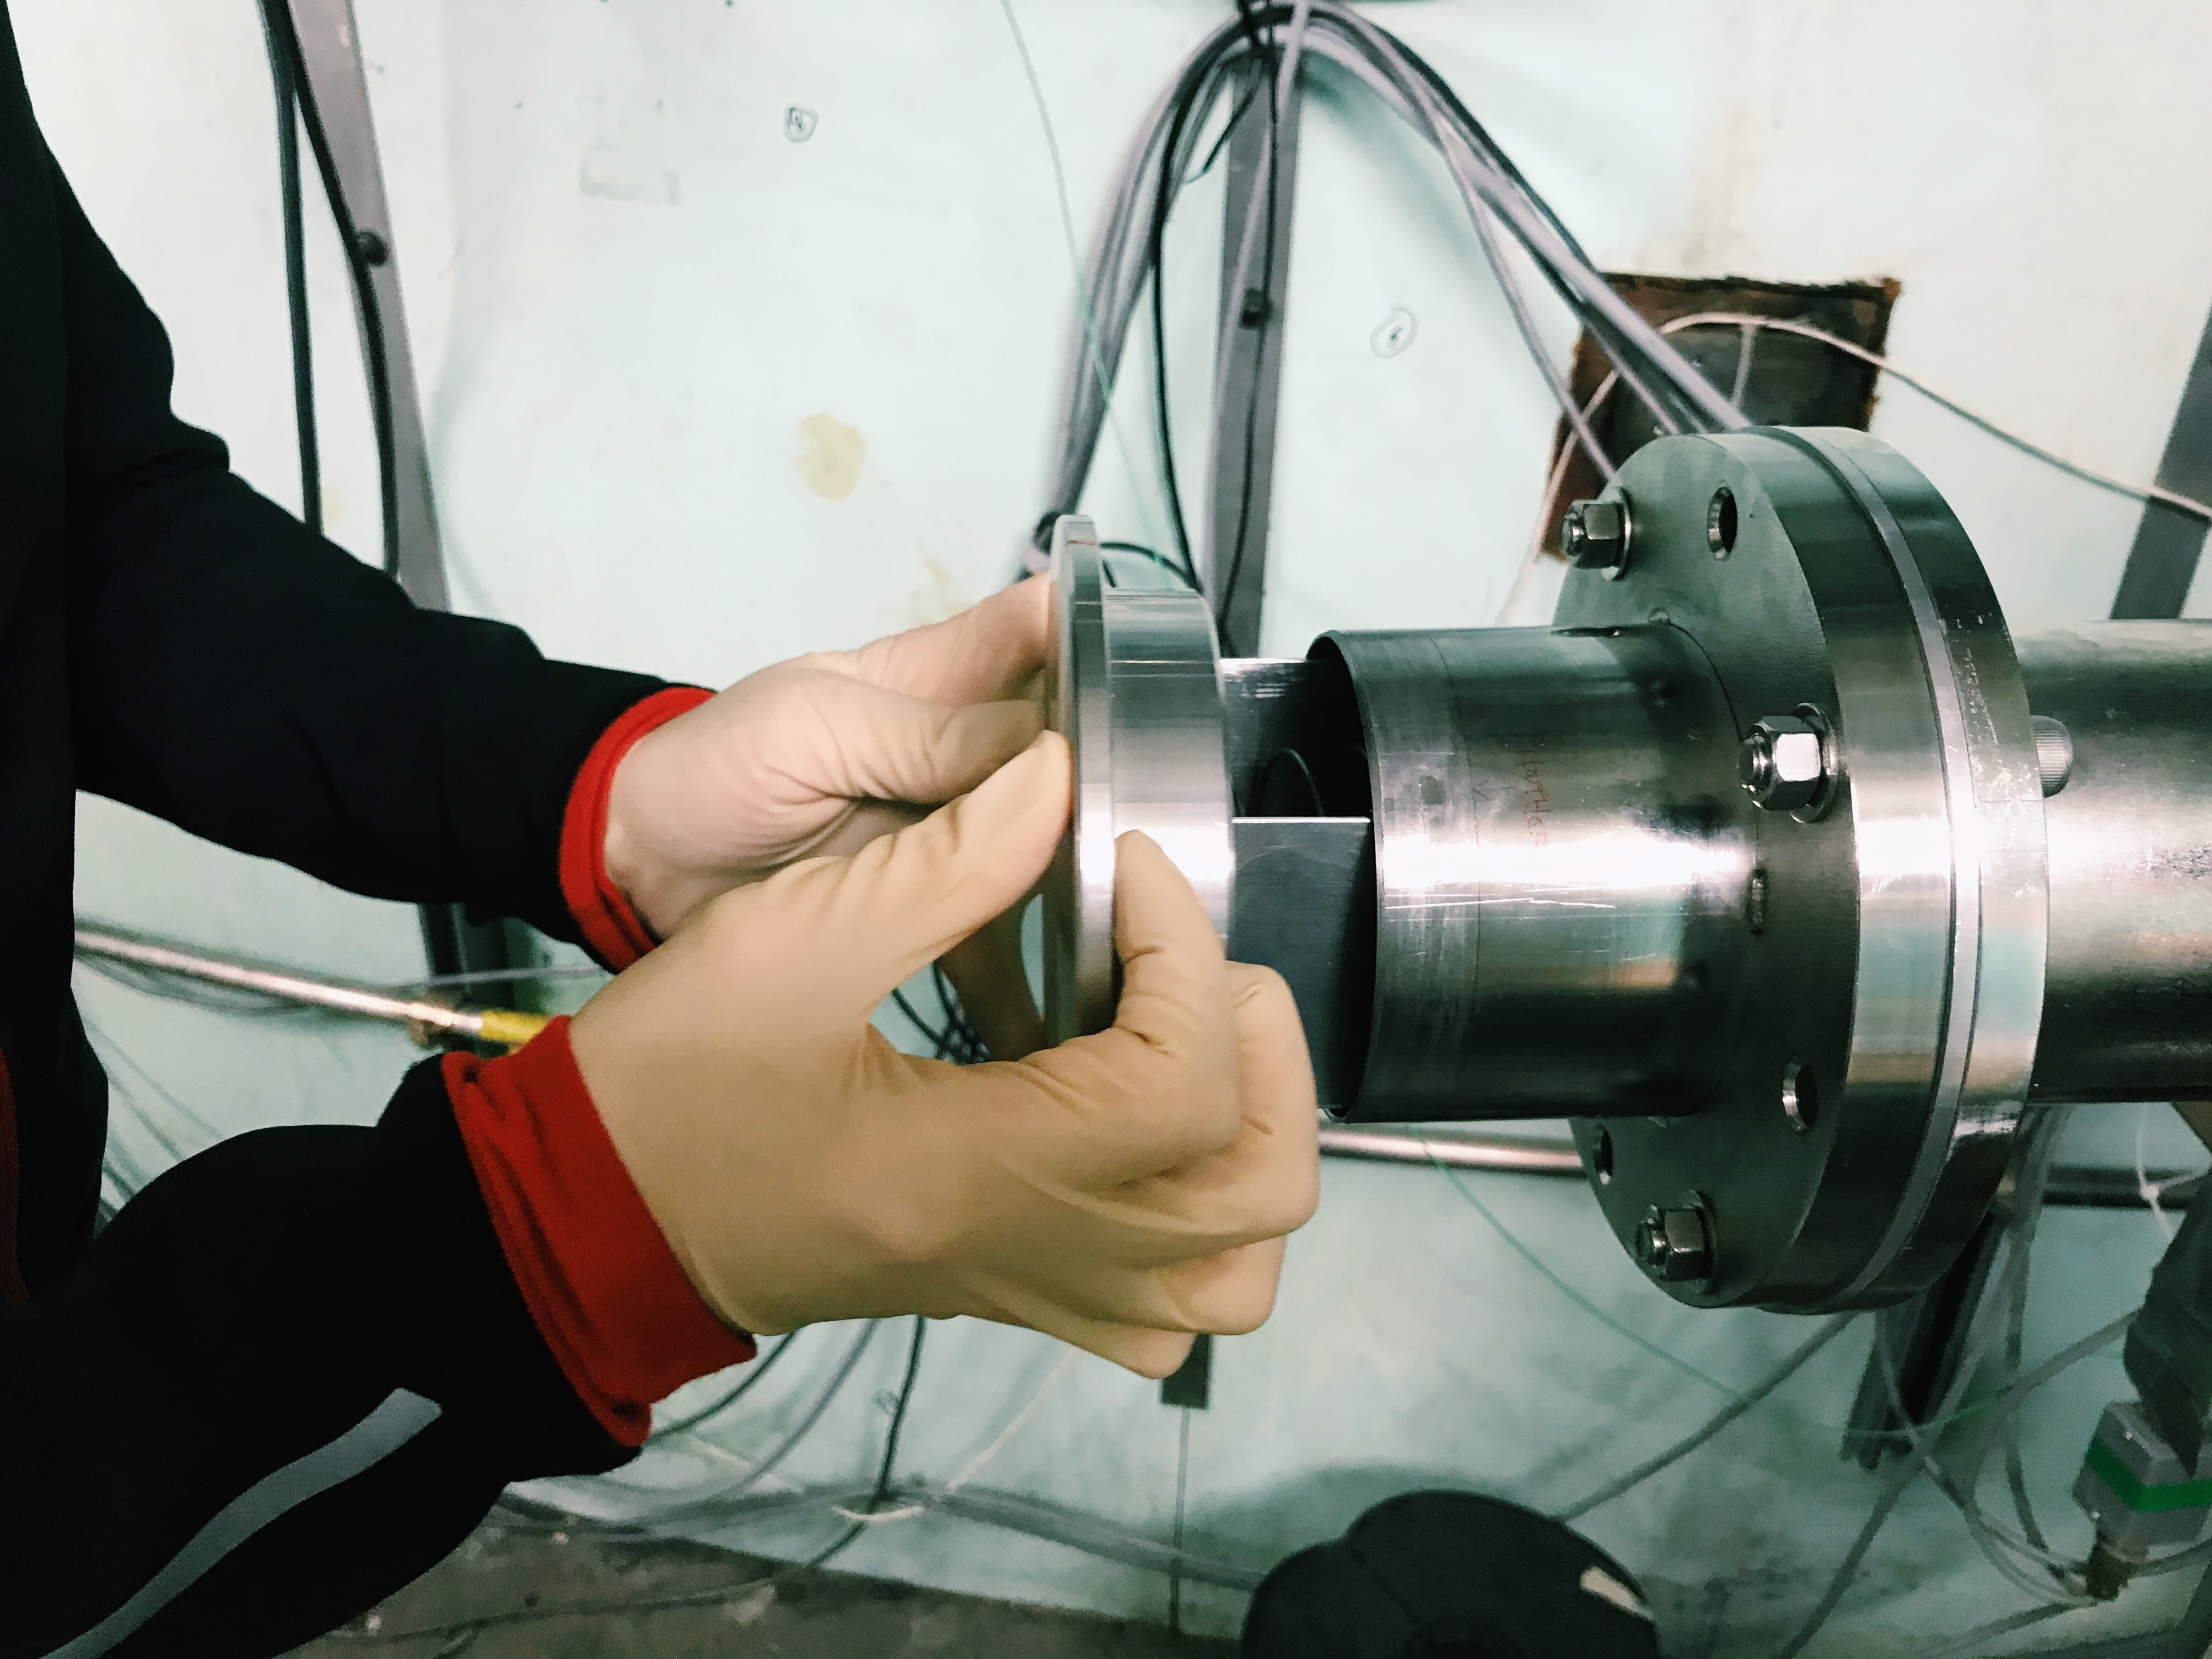
\includegraphics[width=6.6cm]{Experiment/tube.JPG} }}%
    \caption{The figure shows the target stack was placed in the beamline. \textbf{Left:} The targets were placed in a 6061 aluminum alloy targetholder with a hollow center for the beam to pass through. The hollow spring kept the targets on a finite position throughout the irradiation. \textbf{right:} The target holder was placed in the electrically isolated beamline. }%
    \label{fig:targetstack}%
\end{figure}






\subsubsection{Intensity profile of the beam}

After irradiation, Gafchromic film were attached to the activated stainless steel in the front and the back of the stack, to obtain a spatial intensity profile of the beam. The activated film attached to the Gafhromic film can be seen in figure \ref{fig:SS1_gafchromic}. The radius of the activity from stainless on gafchromic film was used in the imaging process program ImageJ-1.52k, which is developed by the National Insititutes of Health and the Laboratory for Optical and Computational Instrumentation \cite{Rasband2010}. The Gafchromic films were scanned alongside a ruler for scale comparison. Since the images are divided into pixels, a 3 \textcolor{red}{(why 3cm?)} cm line segment was drawn alongside the ruler to set the scale to pixels/cm in the program. The intensity over the developed film was obtained by inverting the scanned image, and drawing a line segment along the beam spot that created a position dependent intensity array. The intensity profile can be fitted to a Gaussian, which is shown example-wise in figure \ref{fig:beamprofile}, which is the horizontal beam profile in the front and the back of the stack. In the assumption that the beam was underfilled, it was important to build confidence in that the beamspot was ca. 1 cm in diameter, which was done estimating the full width half maximum of the Gaussian profile. The FWHM over SS1 was 1.2017 cm horizontally ($\sigma^2=$0.2604 cm$^2$) and 1.1420 cm vertically ($\sigma^2=$0.2352 cm$^2$). The FWHM over SS2 was 0.6706 cm horizontally ($\sigma^2=$0.0811 cm$^2$) and 0.5783 cm vertically ($\sigma^2=$0.0603 cm$^2$). \\

\textcolor{red}{Normally the beam broadens throughout the stack due to scattering. As we can see, this not the case, since the beam is stopped in the targetstack, and therefor we do not know how much the beam truly scatters. This gives a higher uncertainty.  
The stainless steel (which consist of ..) has fast decay time. However since it emits beta-particles, the radius will slightly increase, and the true beam spot is slightly smaller. Thus the estimated FWHM values for SS1  seems to be within the criterion for underfilled targets. }



\begin{figure}
    \centering
    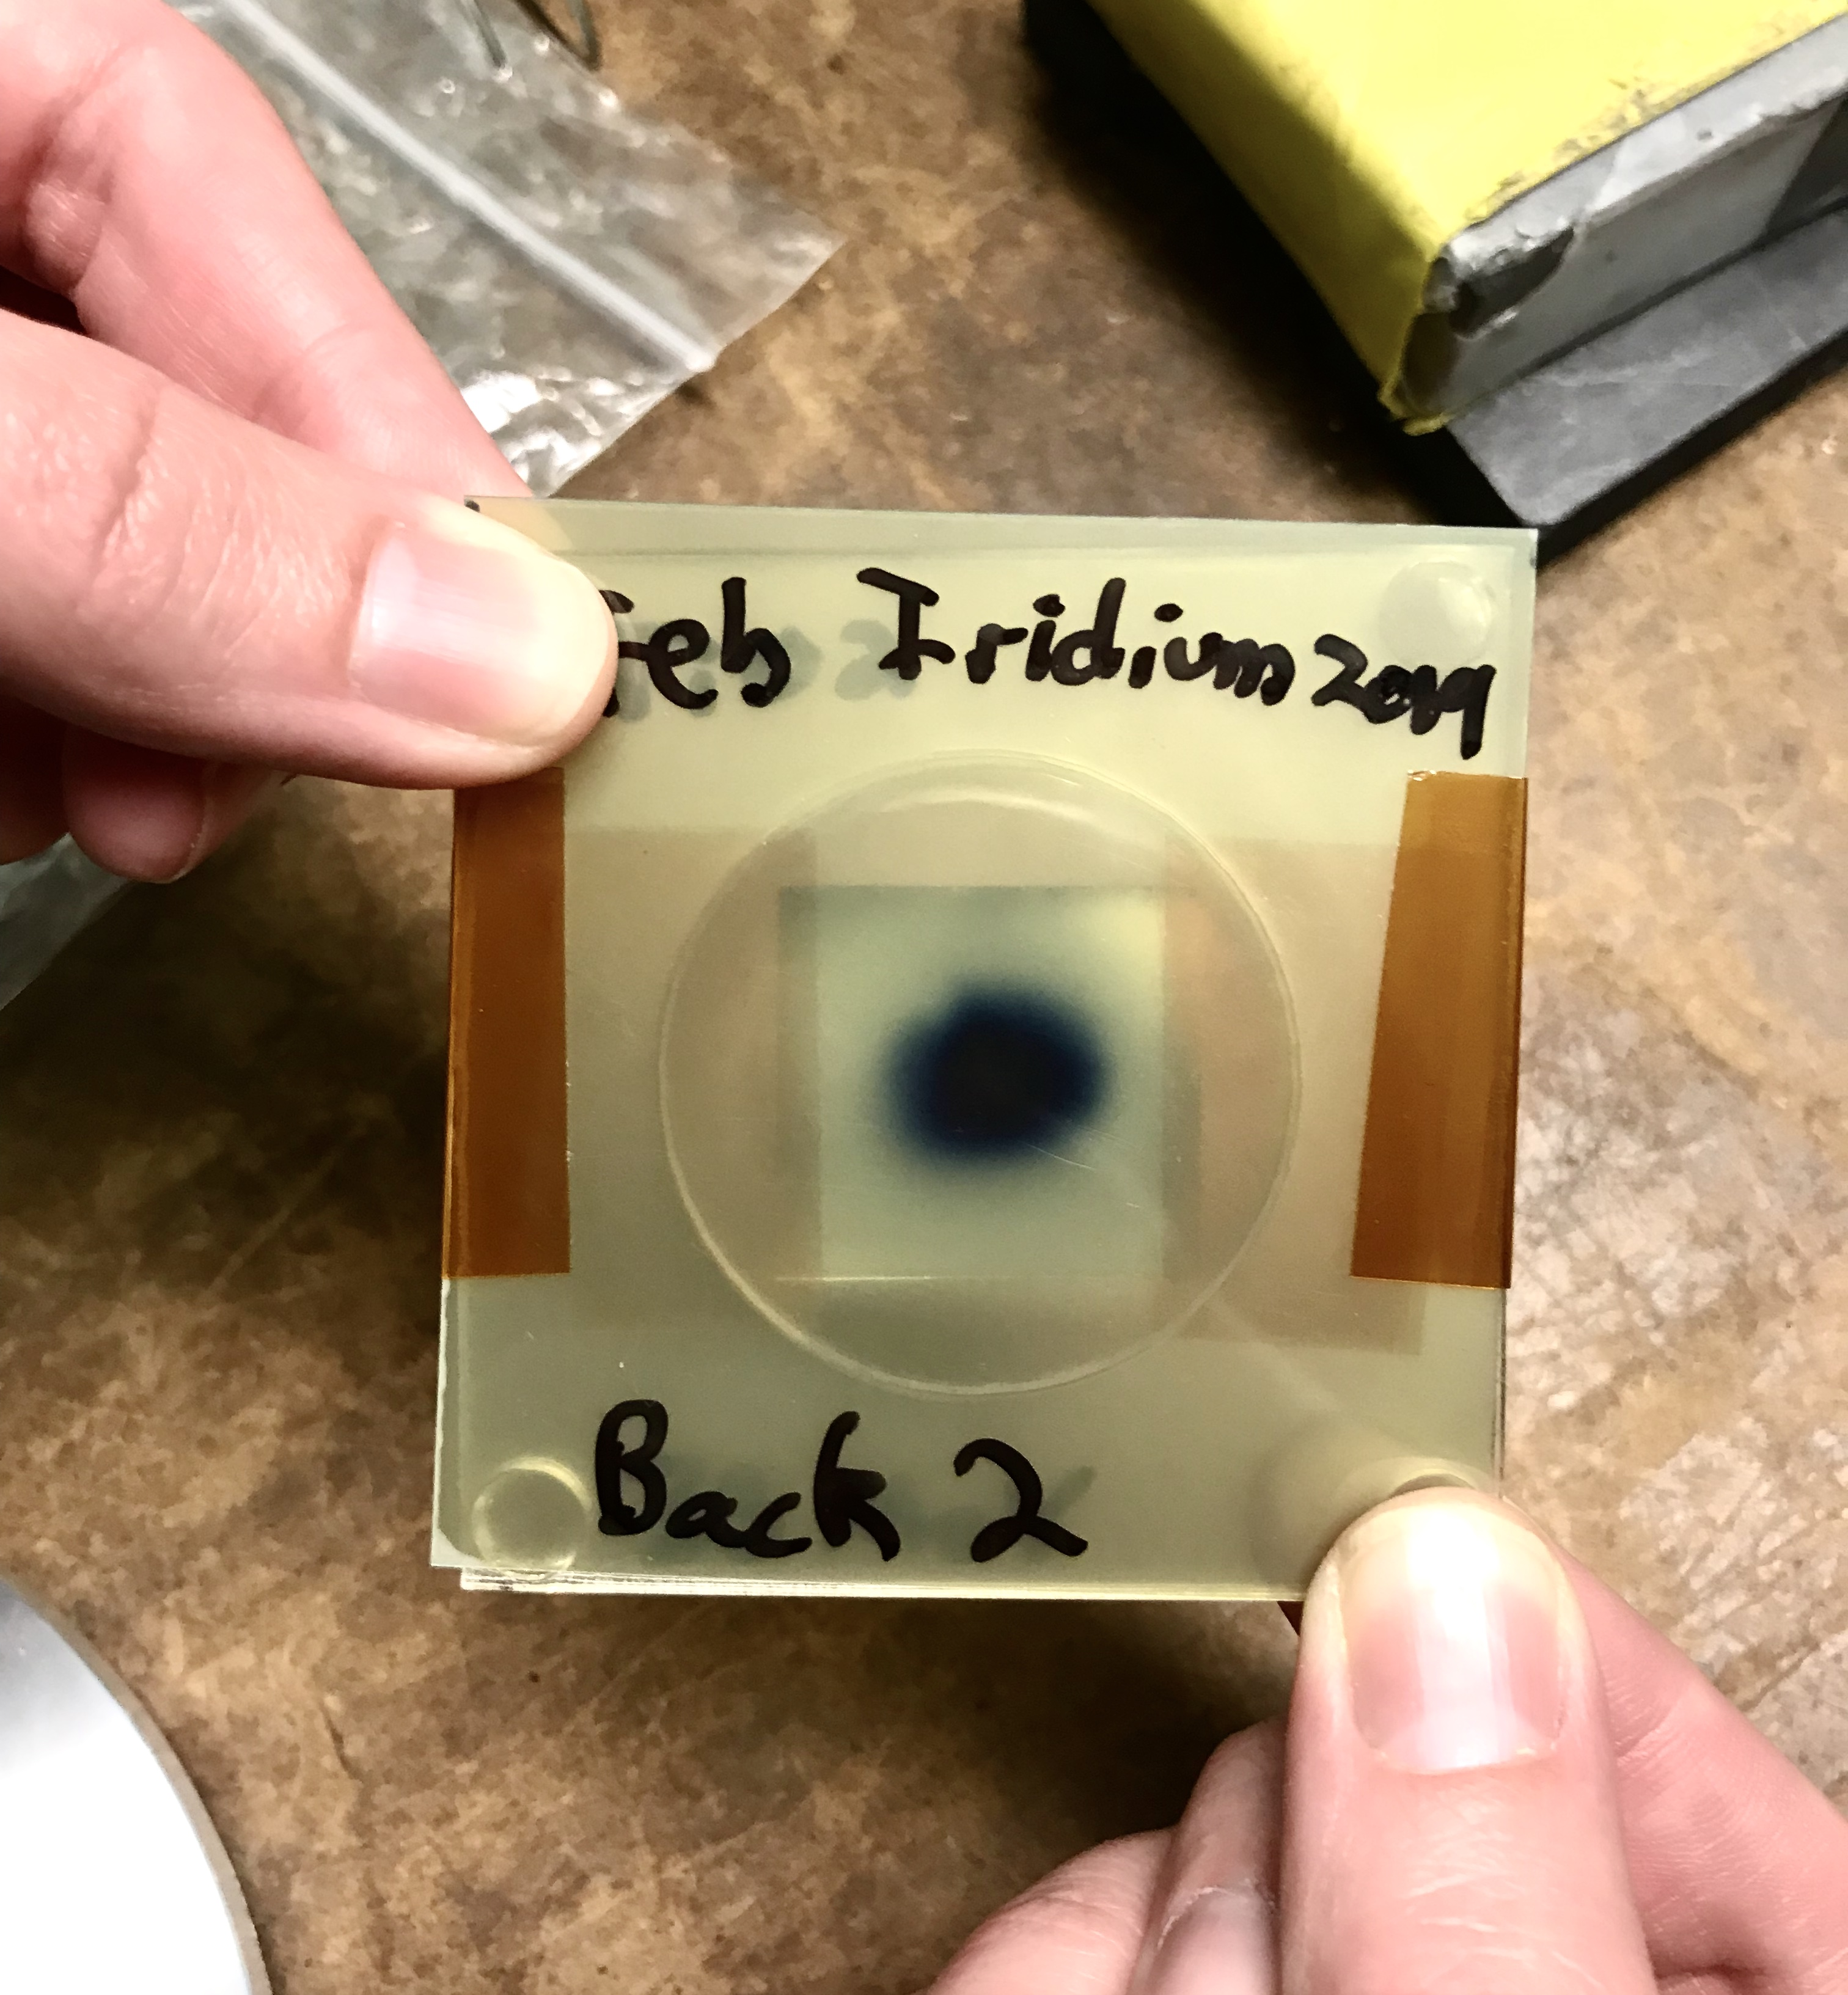
\includegraphics[width=0.3\textwidth]{Experiment/gafchromic_beamprofile.jpg}
    \caption{The gafcromic film on the activated SS1 foil. }
    \label{fig:SS1_gafchromic}
\end{figure}

\begin{figure}%
    \centering
    \subfloat[Horizontal intensity profile of SS1]{{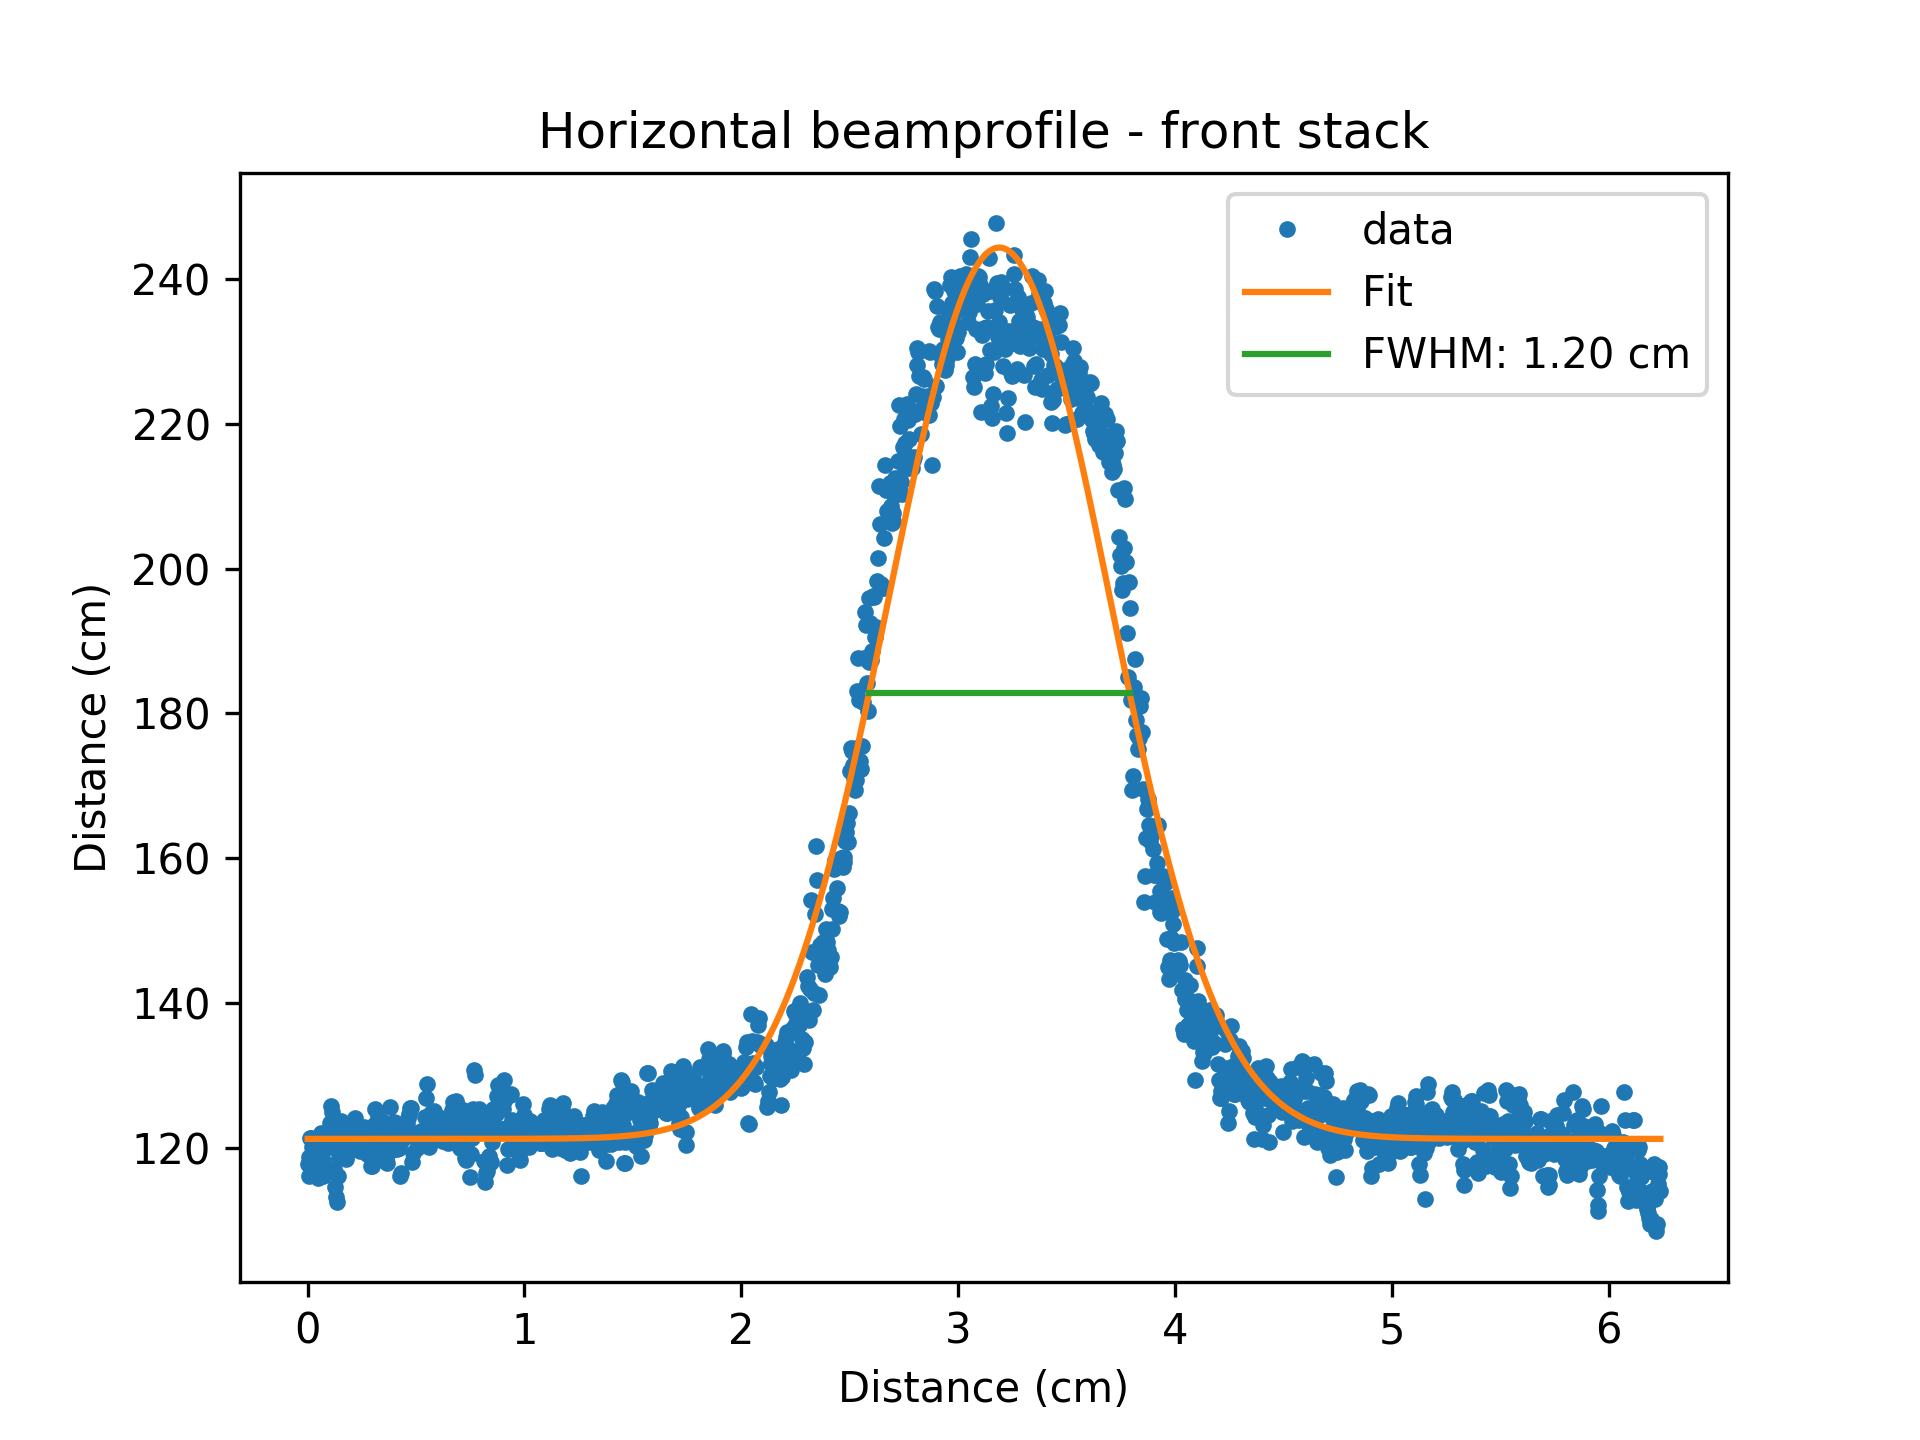
\includegraphics[width=6.6cm]{Experiment/ss_front_h.png} }}%
    
    \quad
    \subfloat[Horizontal intensity profile at SS2]{{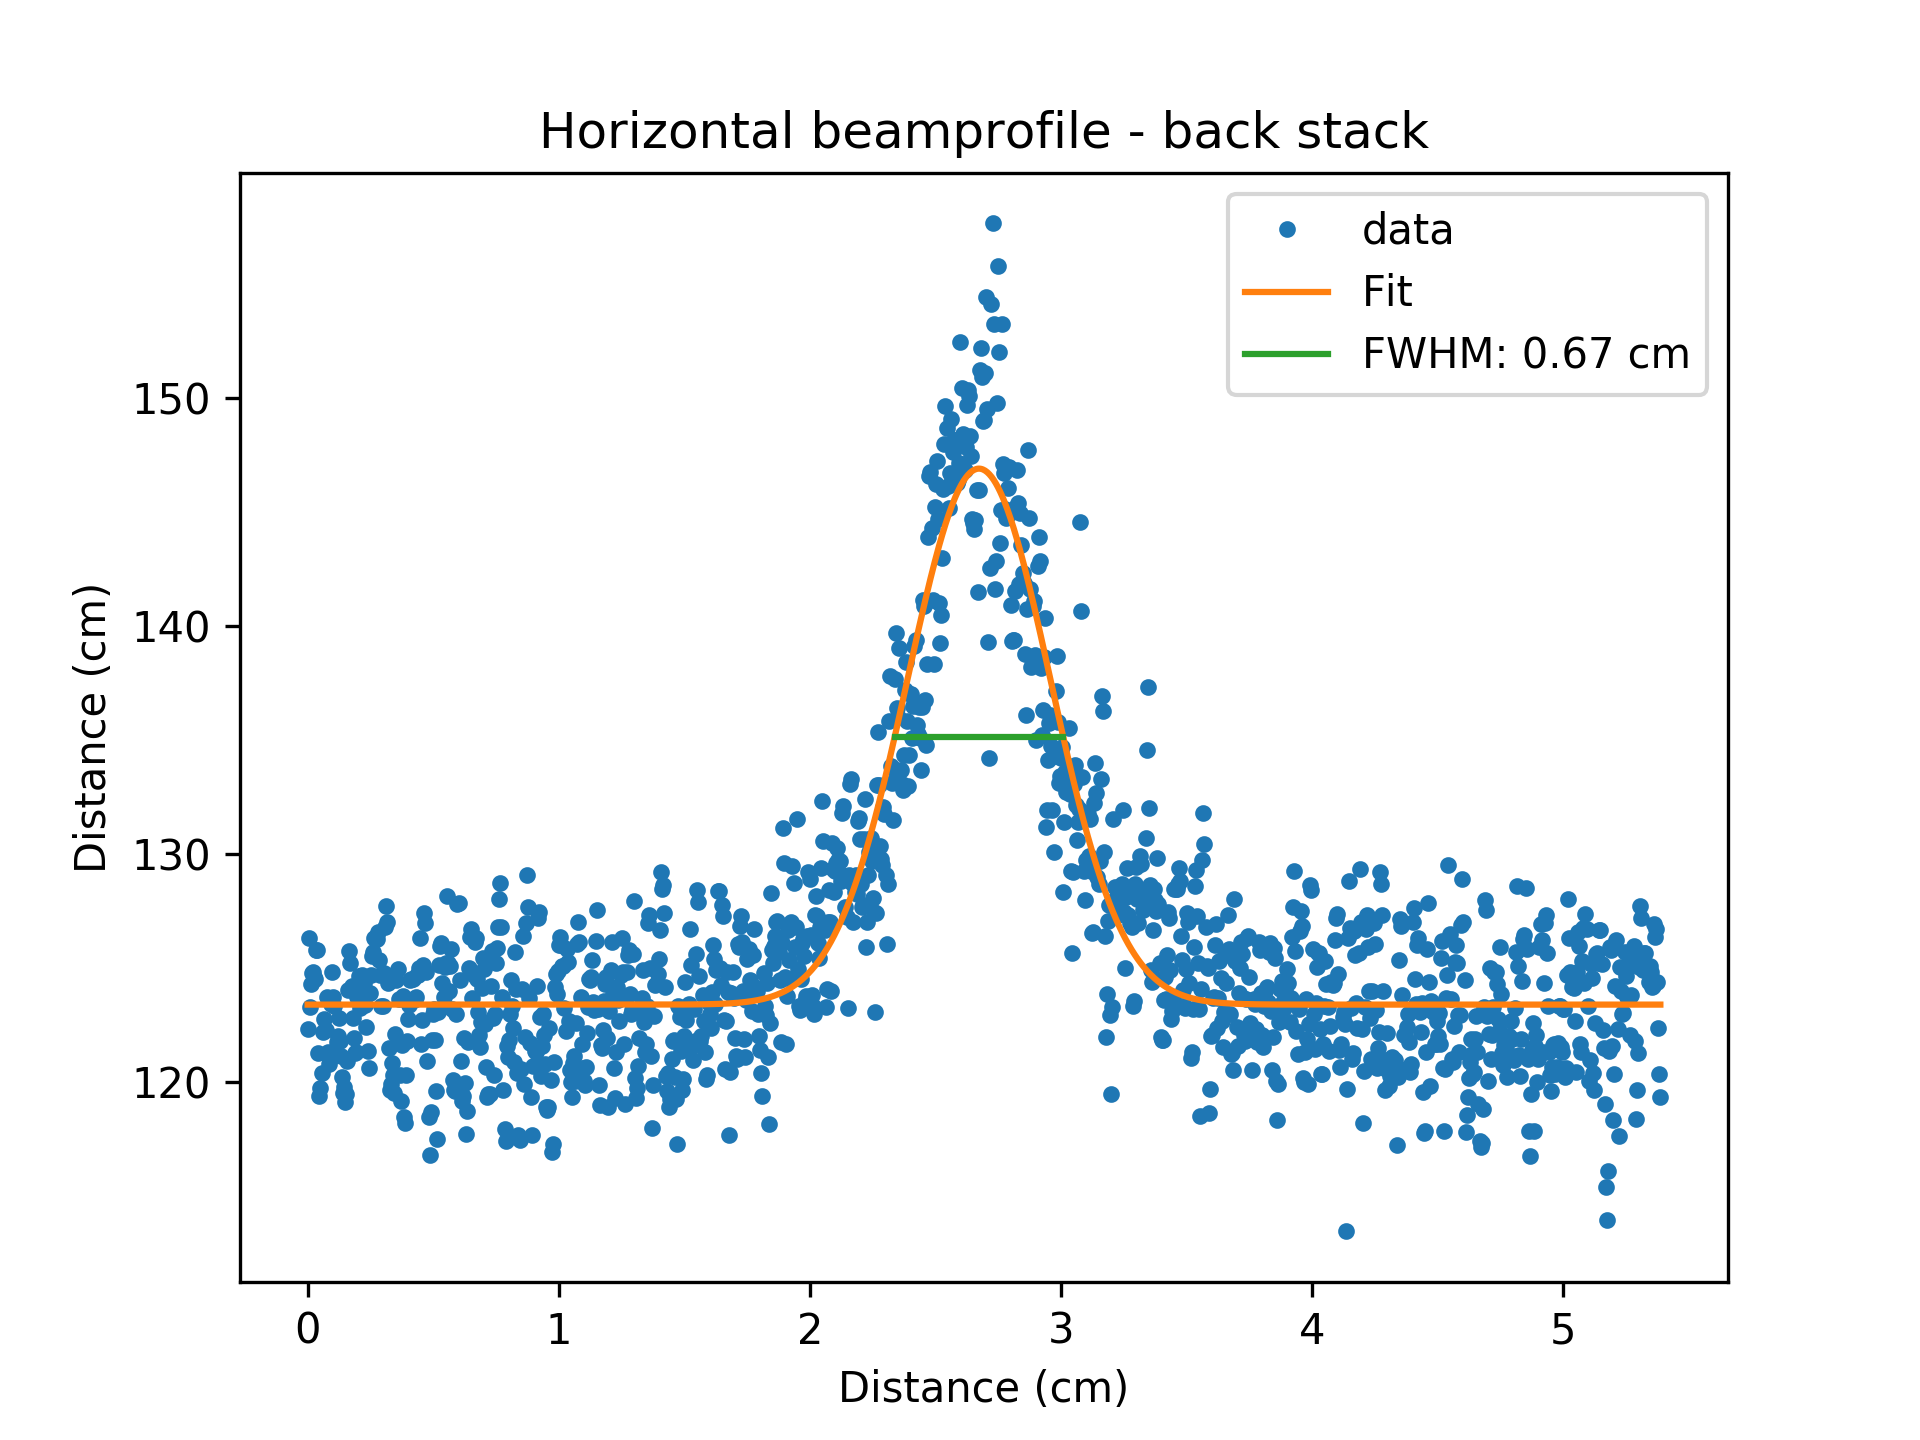
\includegraphics[width=6.6cm]{Experiment/ss_back_h.png} }}%
    \caption{Figure shows the intensity profile of the deuteron beam in the front and in the back of the stack horizontally.}%
    \label{fig:beamprofile}%
\end{figure}




\begin{comment}
\begin{table}[]
    \centering
    \caption{Table shows the geometry of the different detectors. }
    \begin{tabular}{|c|c|c|}
        \hline\textbf{}
        Detector & Geometry & Dimension \\
        \hline 
        \makecell{Detector 1} & \makecell{..} & \makecell{..} \\
        \makecell{Detector 1} & \makecell{..} & \makecell{..} \\      
        \makecell{Detector 3} & \makecell{..} & \makecell{..} \\     
        \makecell{Detector 4} & \makecell{..} & \makecell{..} \\  
        \makecell{Detector 5} & \makecell{..} & \makecell{..} \\    
        \makecell{Detector 6} & \makecell{..} & \makecell{..} \\      
        \makecell{Detector 7} & \makecell{..} & \makecell{..} \\     
        \hline
    \end{tabular}
    \label{tab:detector_characteristics}
\end{table}
\end{comment}

\



\begin{comment}
\begin{figure}%
    \centering
    \subfloat[]{{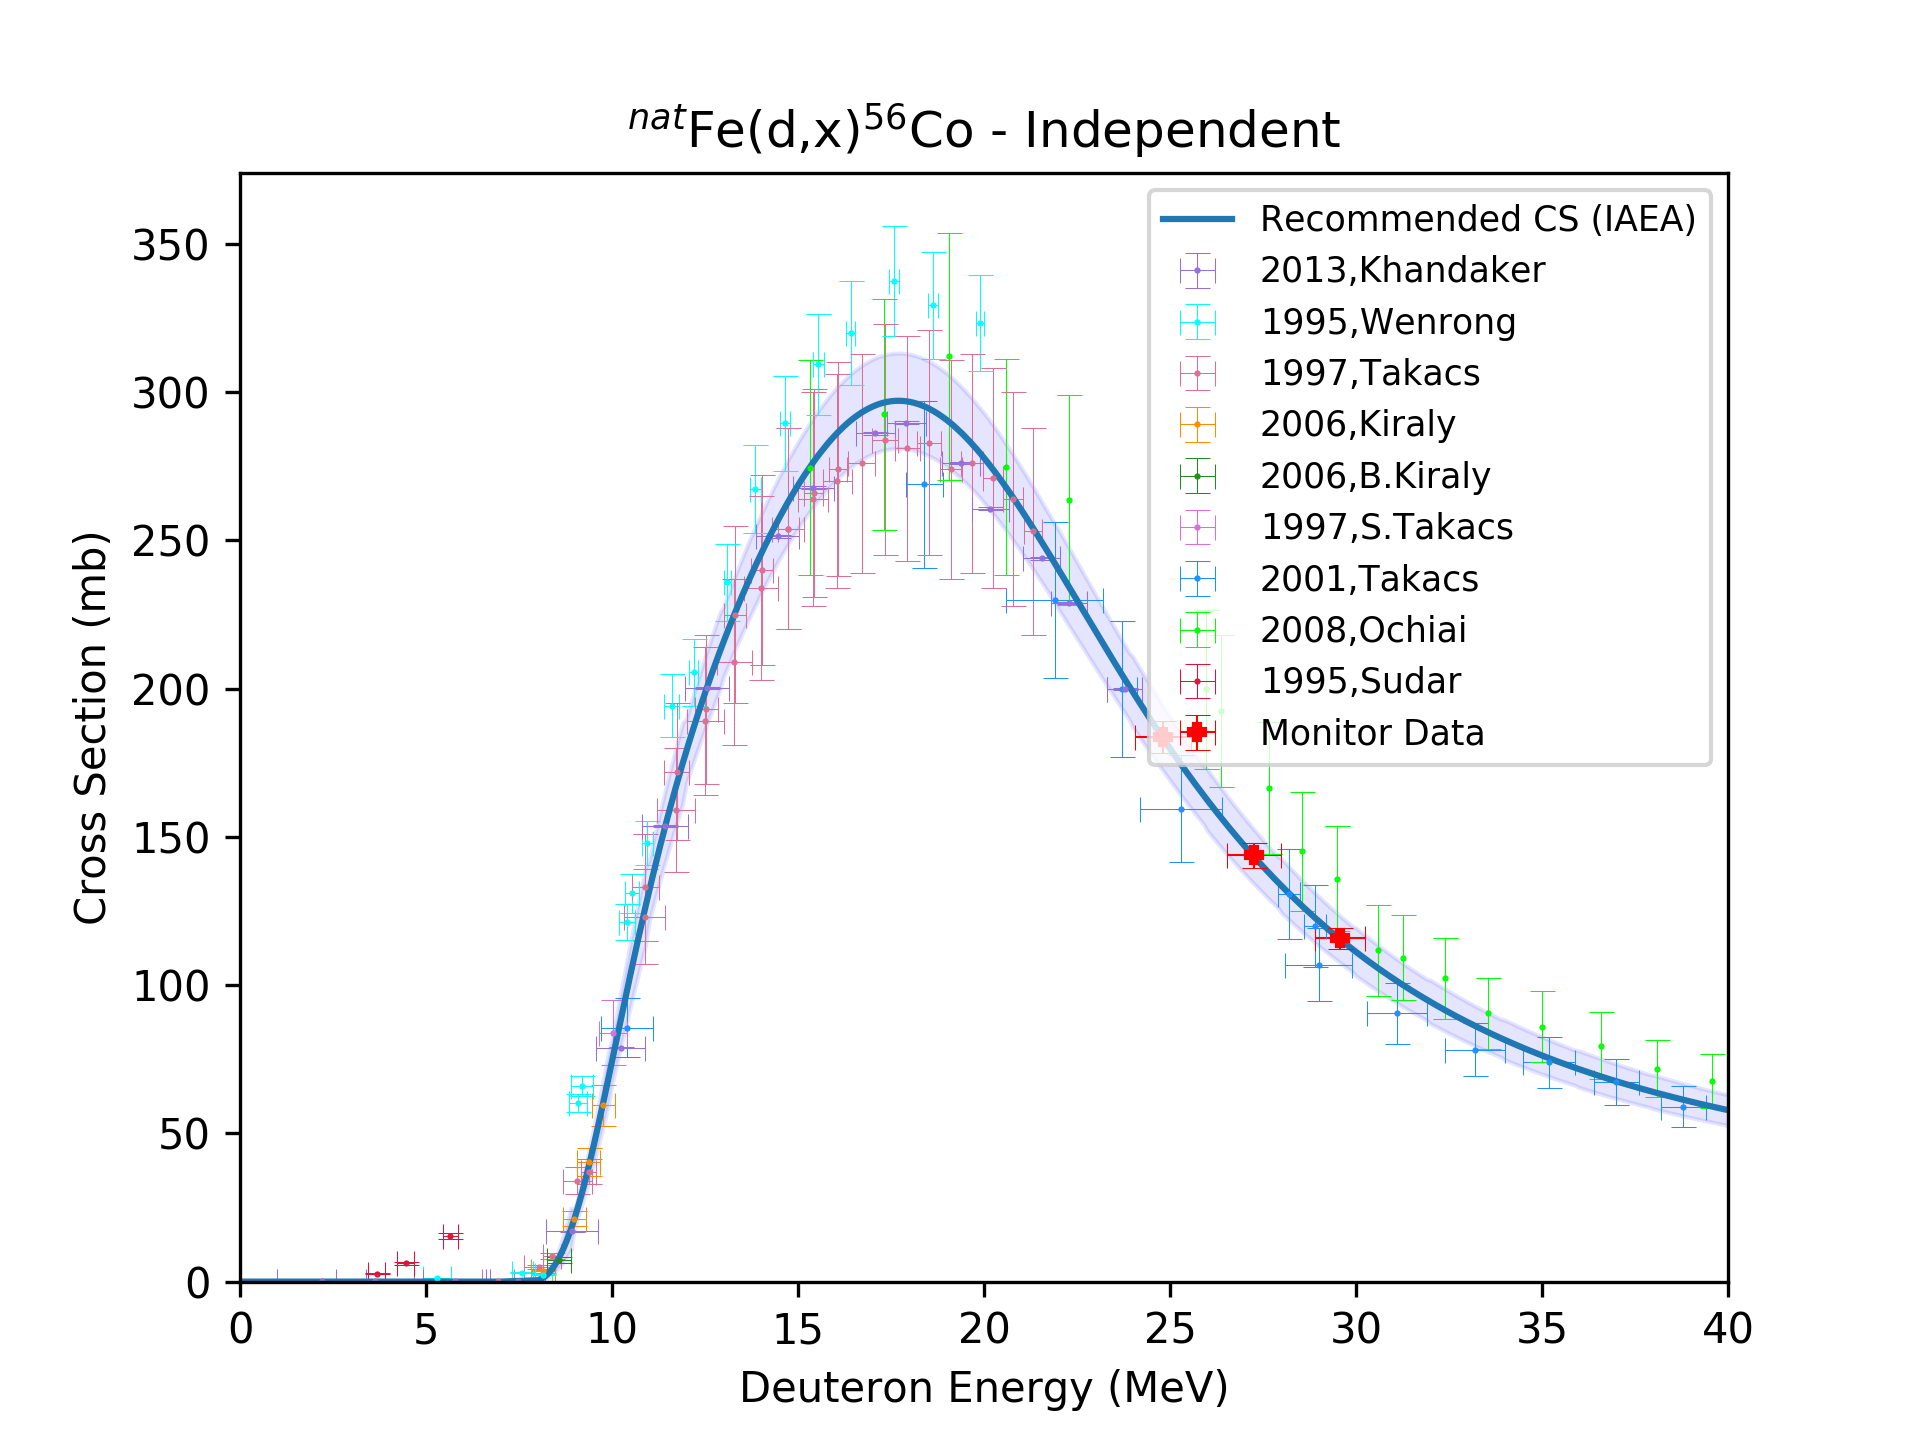
\includegraphics[width=5cm]{Fe_56Co.png} }}%
    \quad
    \subfloat[]{{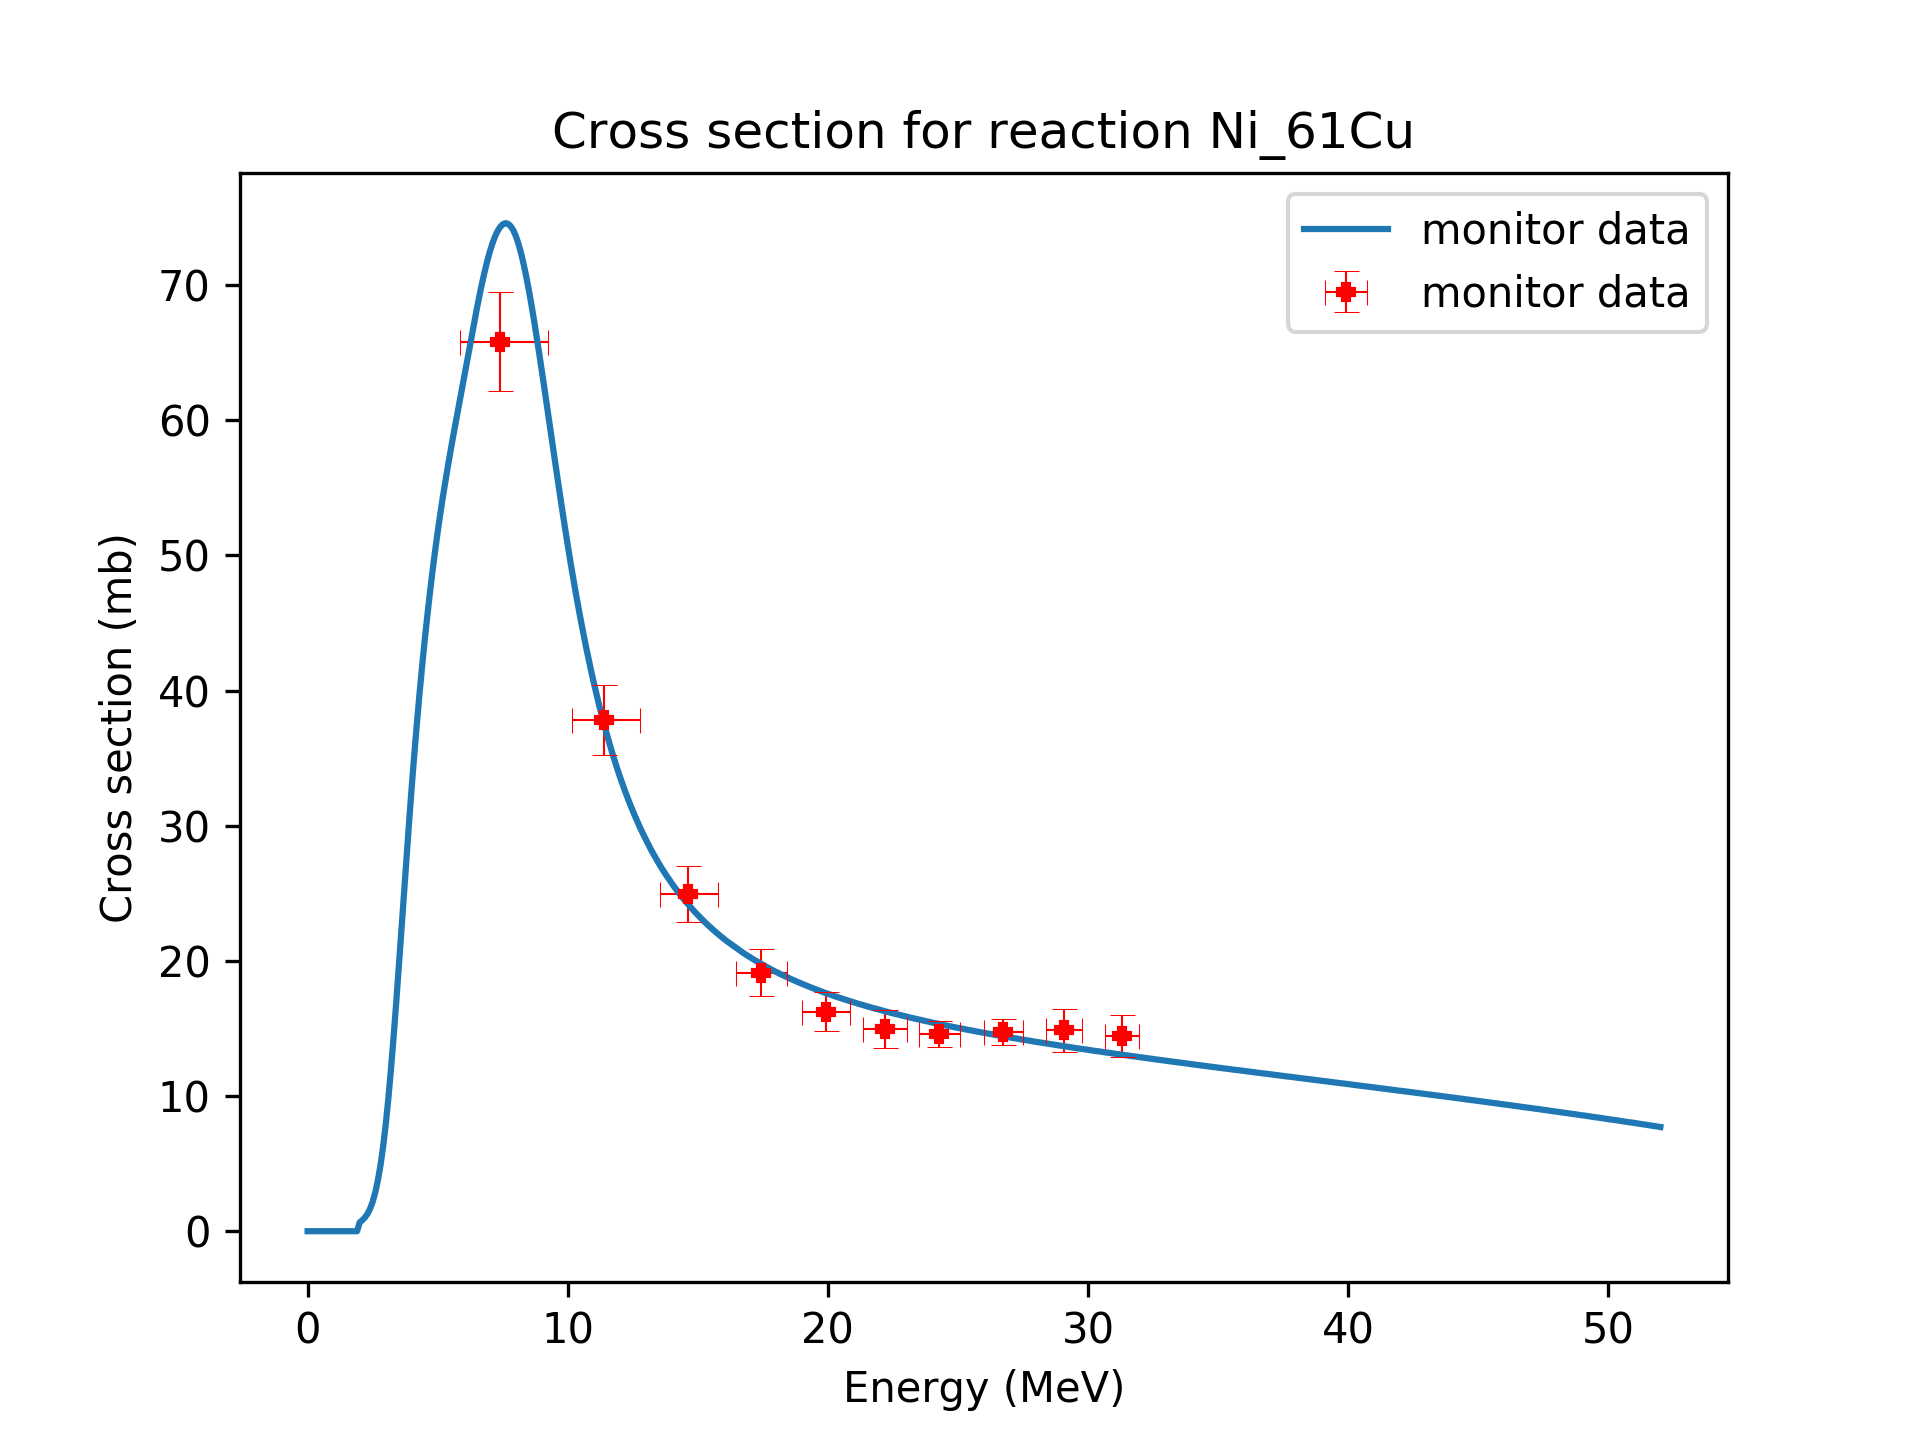
\includegraphics[width=5cm]{Ni_61Cu.png} }}%
    \subfloat[]{{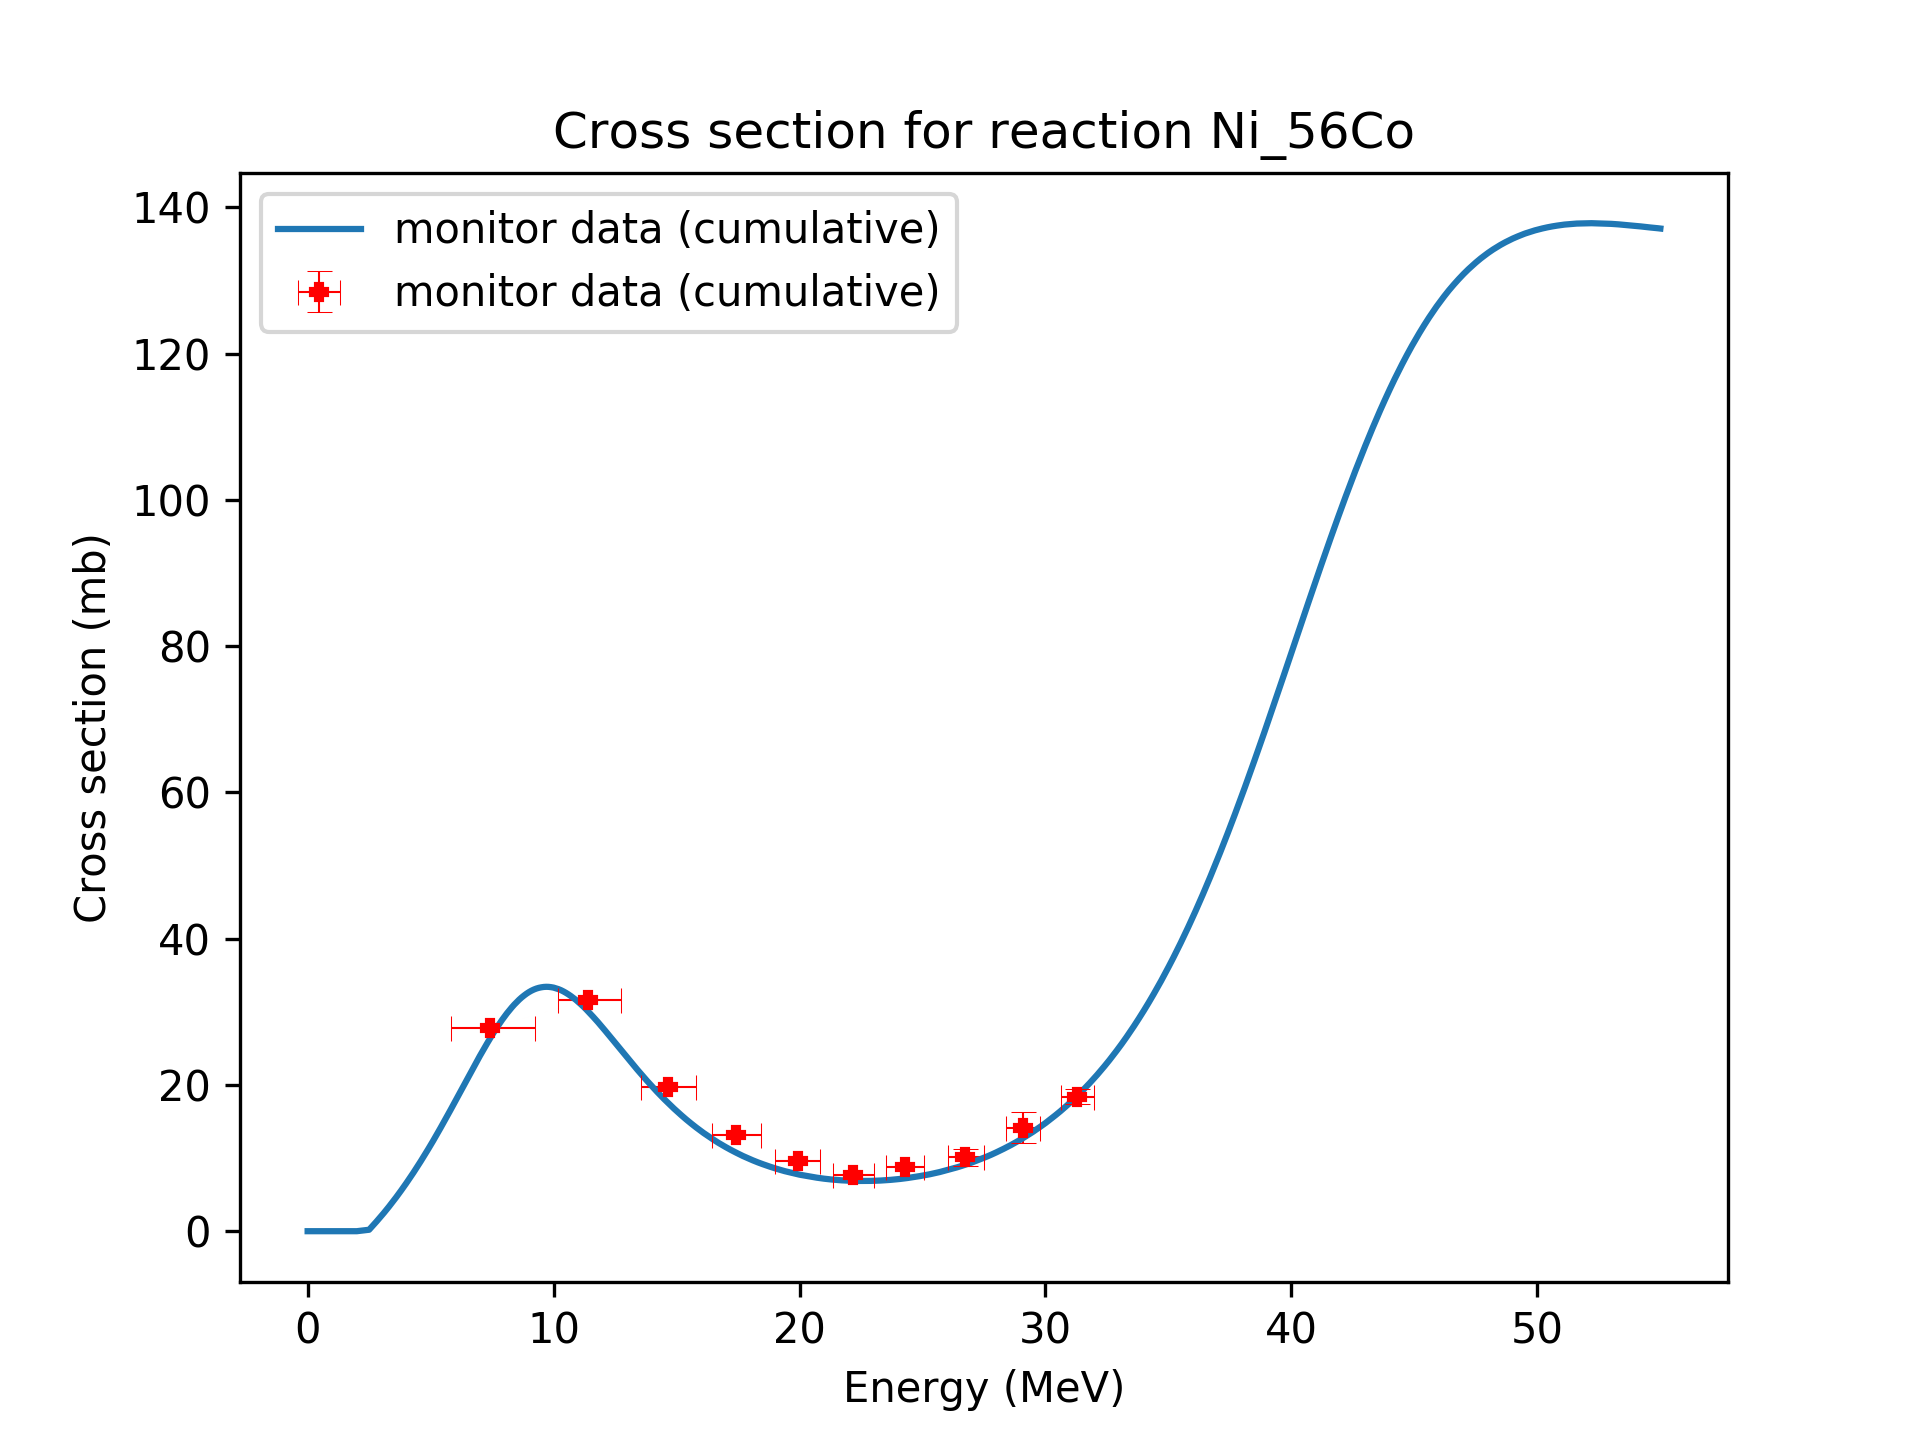
\includegraphics[width=5cm]{Ni_56Co.png} }}%
    \quad
    \subfloat[]{{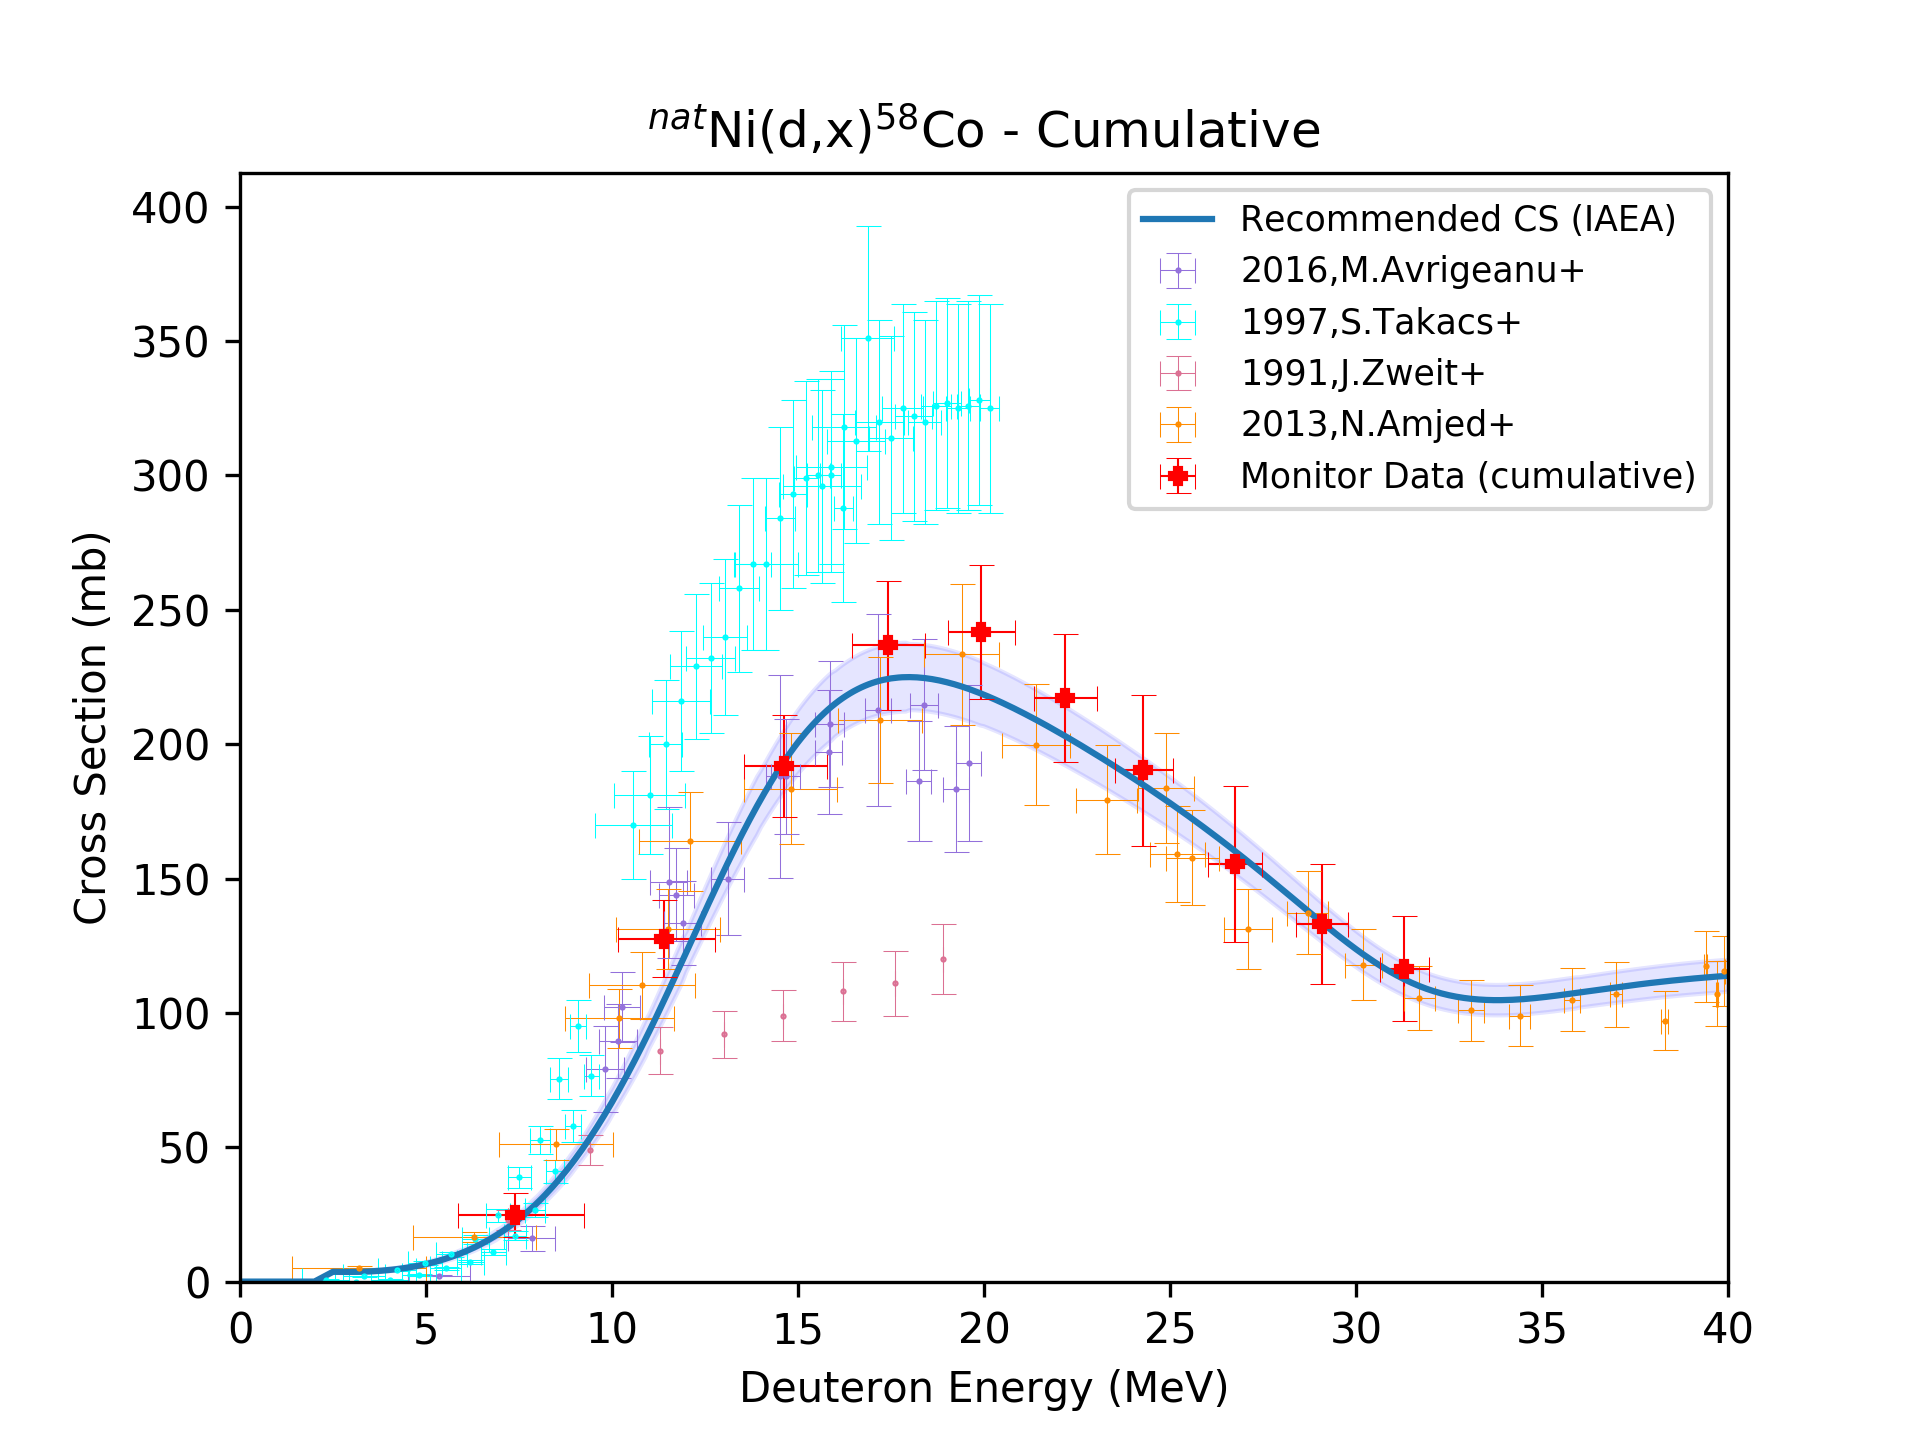
\includegraphics[width=5cm]{Ni_58Co.png} }}%
    \quad
    \subfloat[caption]{{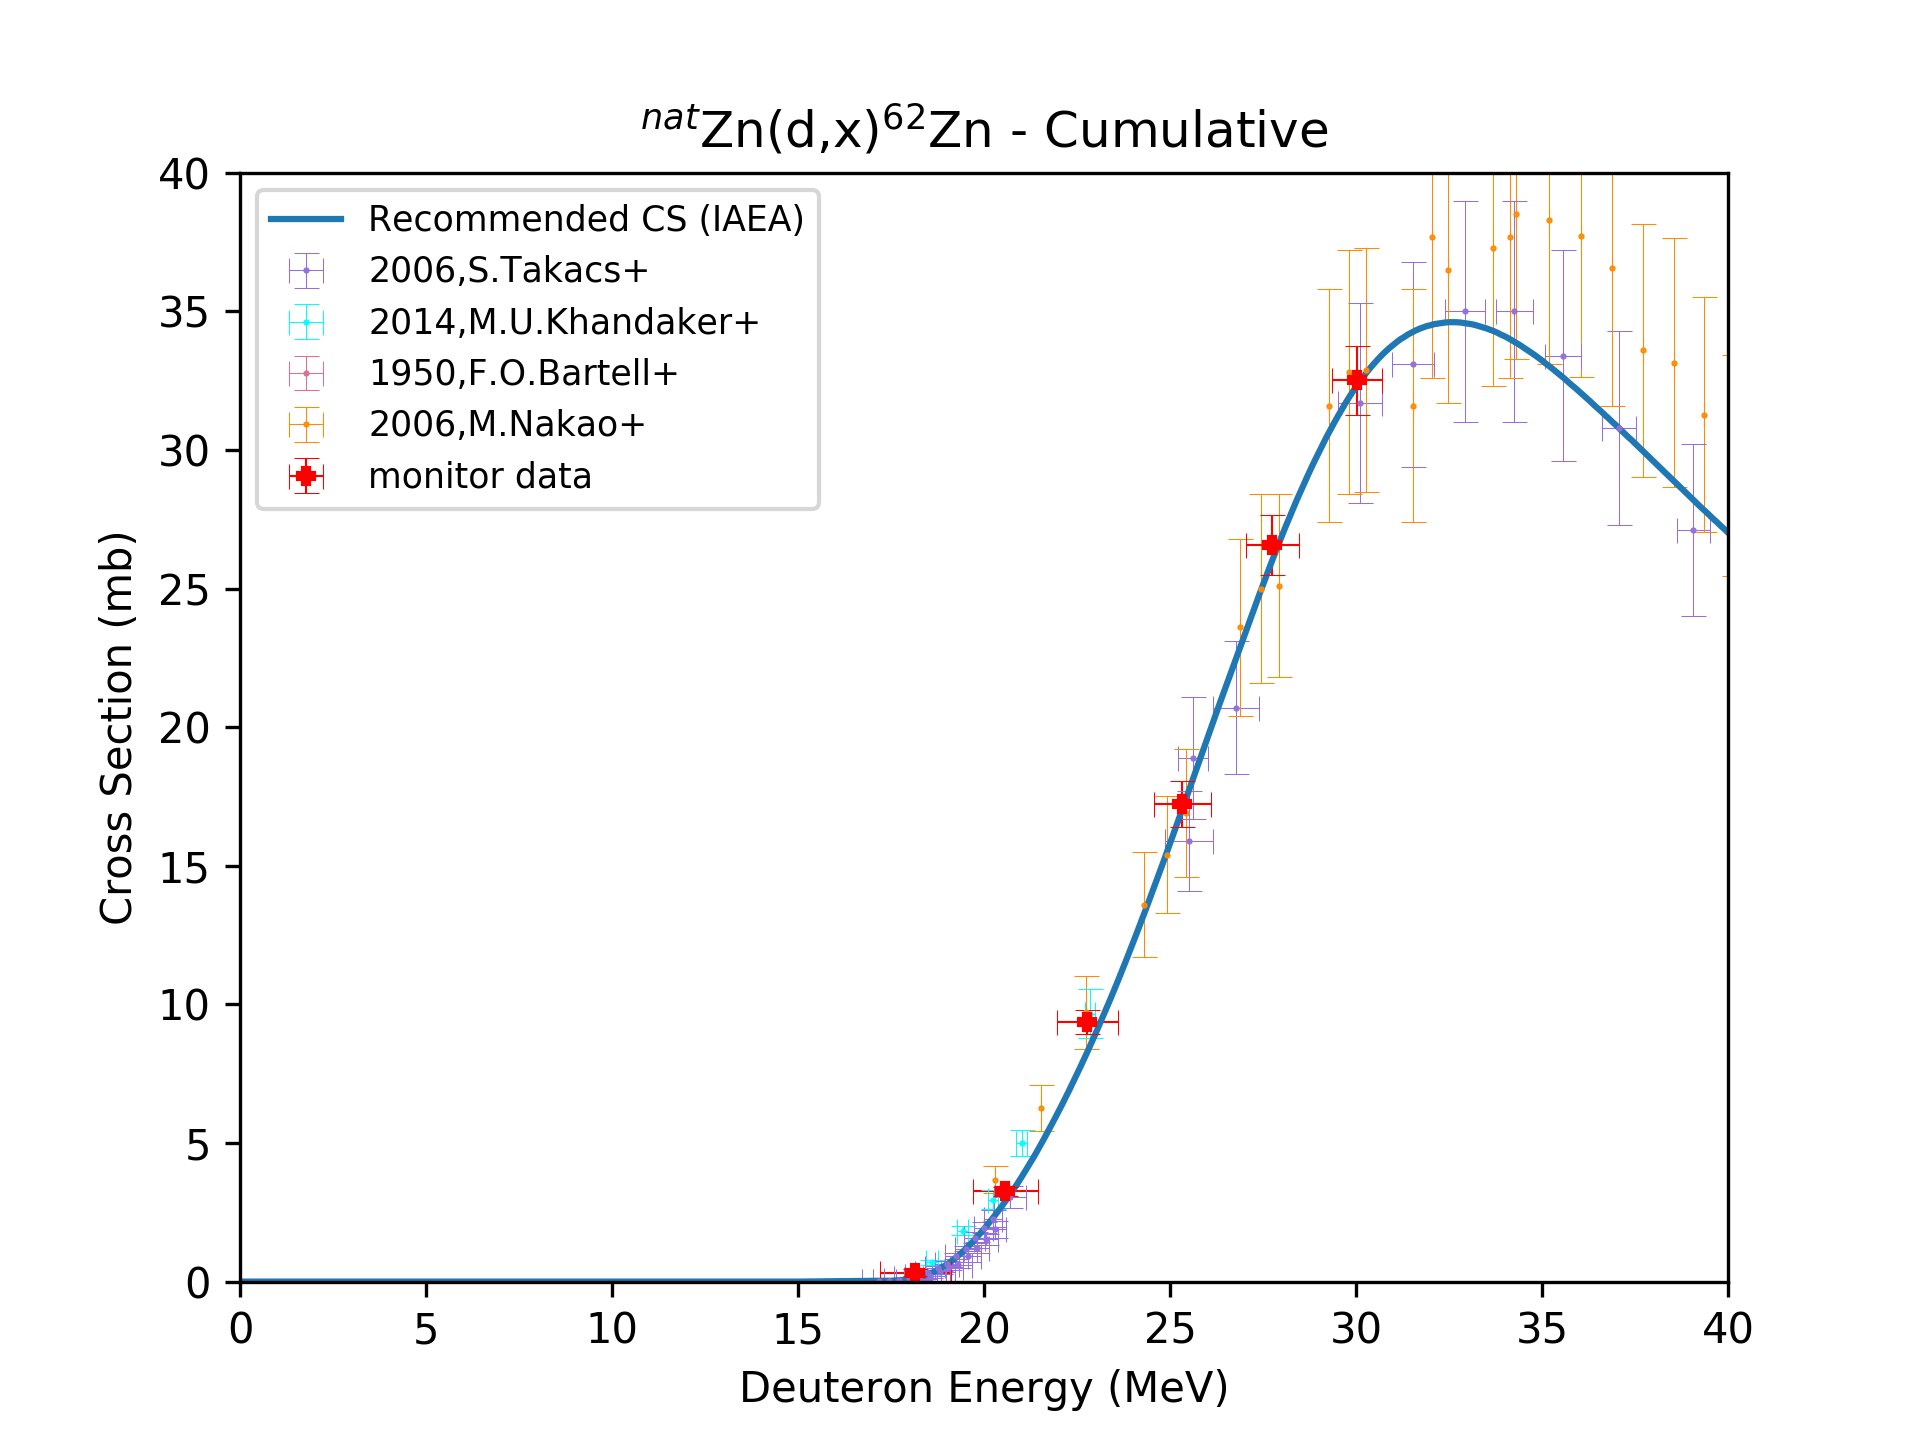
\includegraphics[width=5cm]{Cu_62Zn.png} }}%
    \quad
    \subfloat[]{{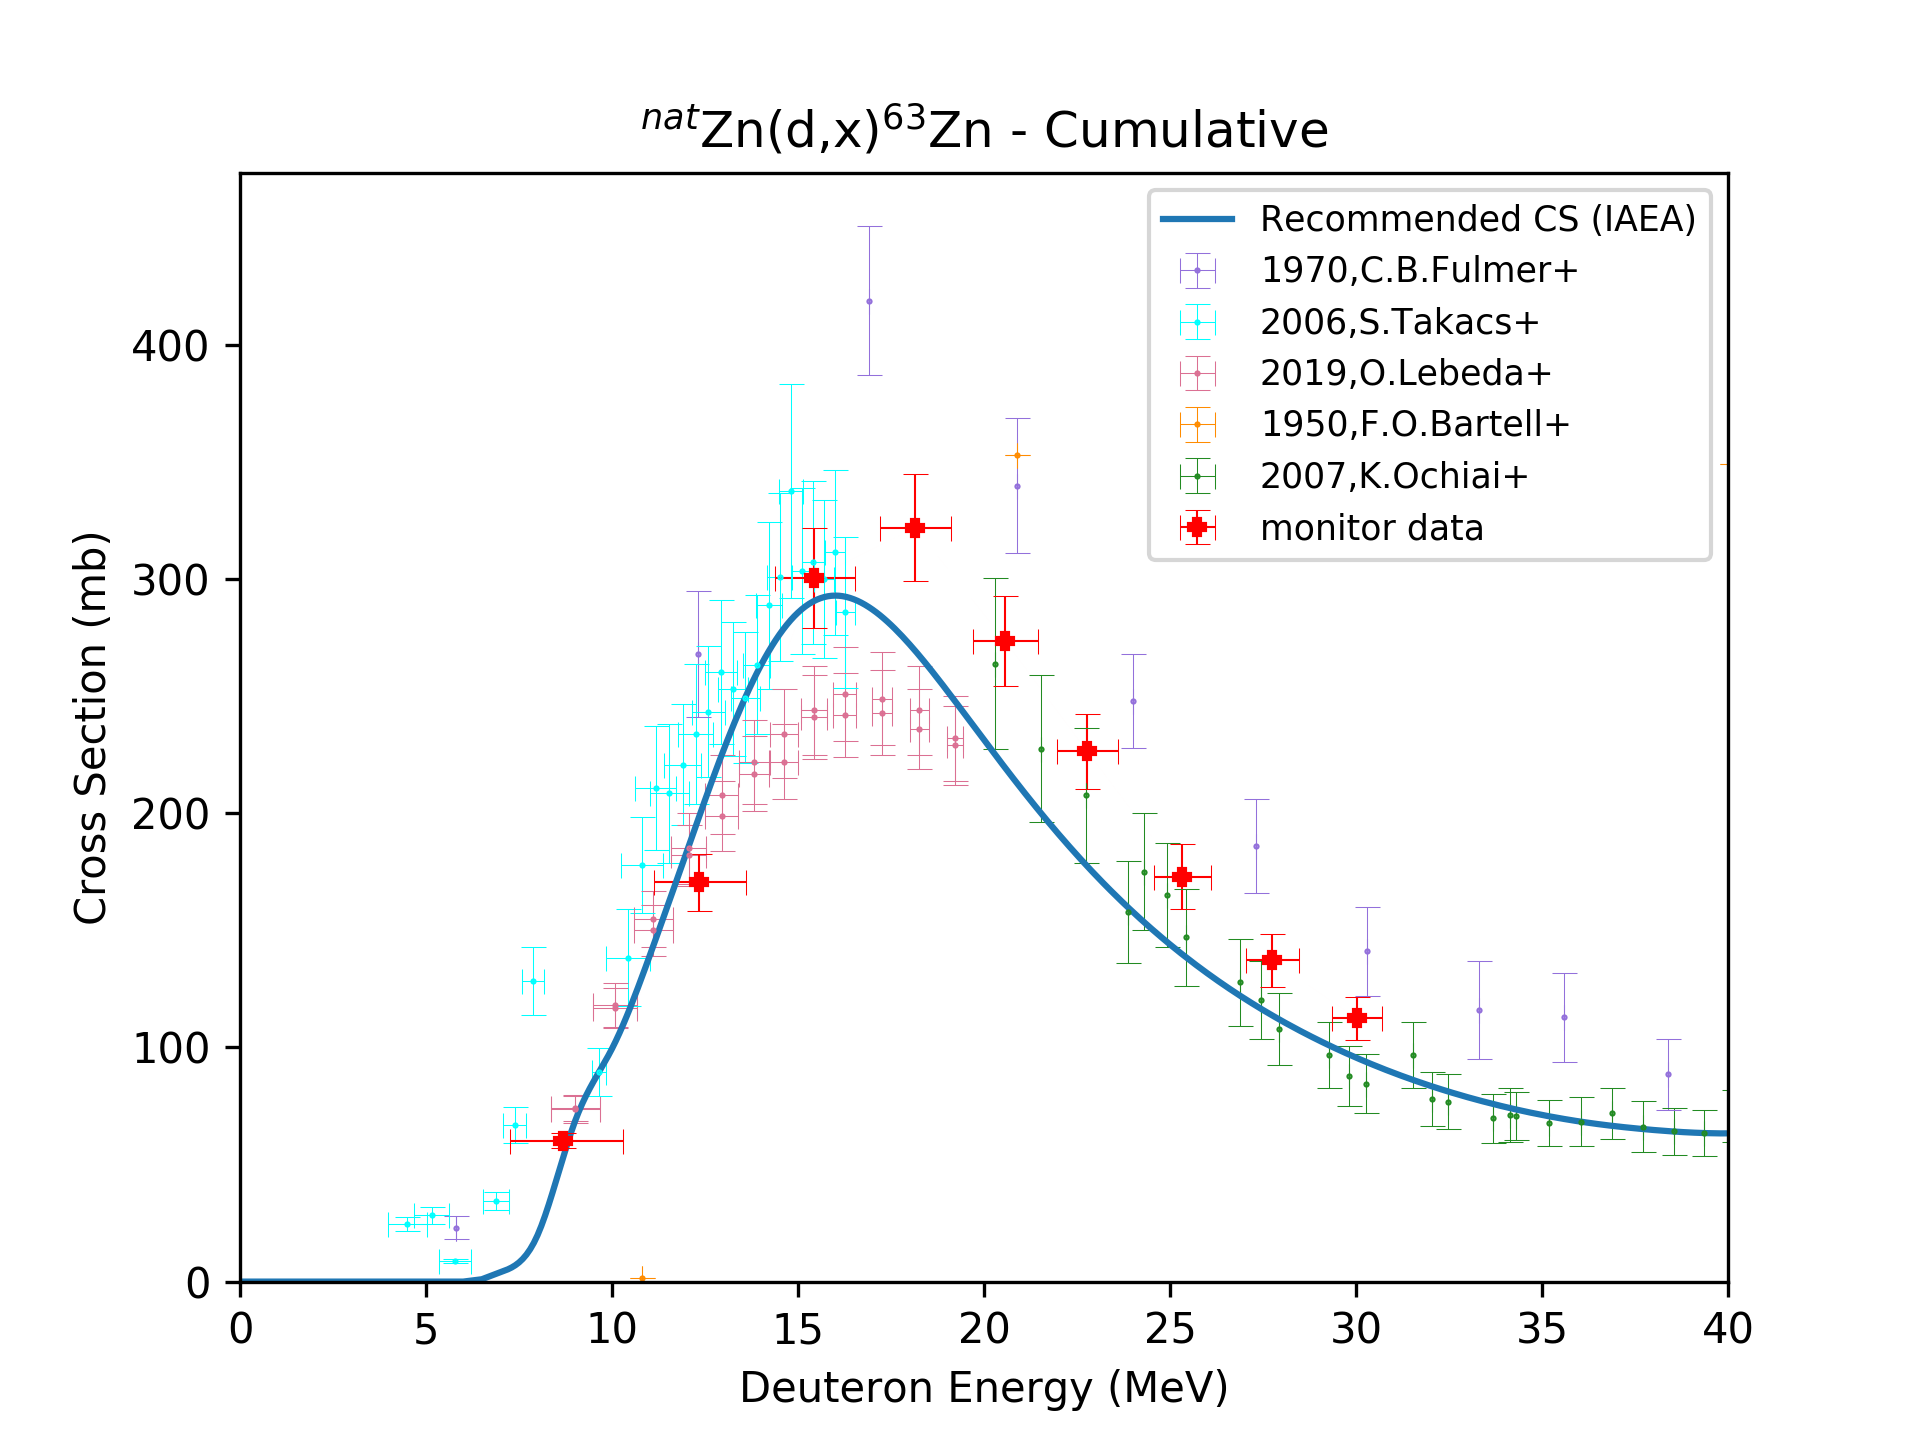
\includegraphics[width=5cm]{Cu_63Zn.png} }}%
    \quad
    \subfloat[]{{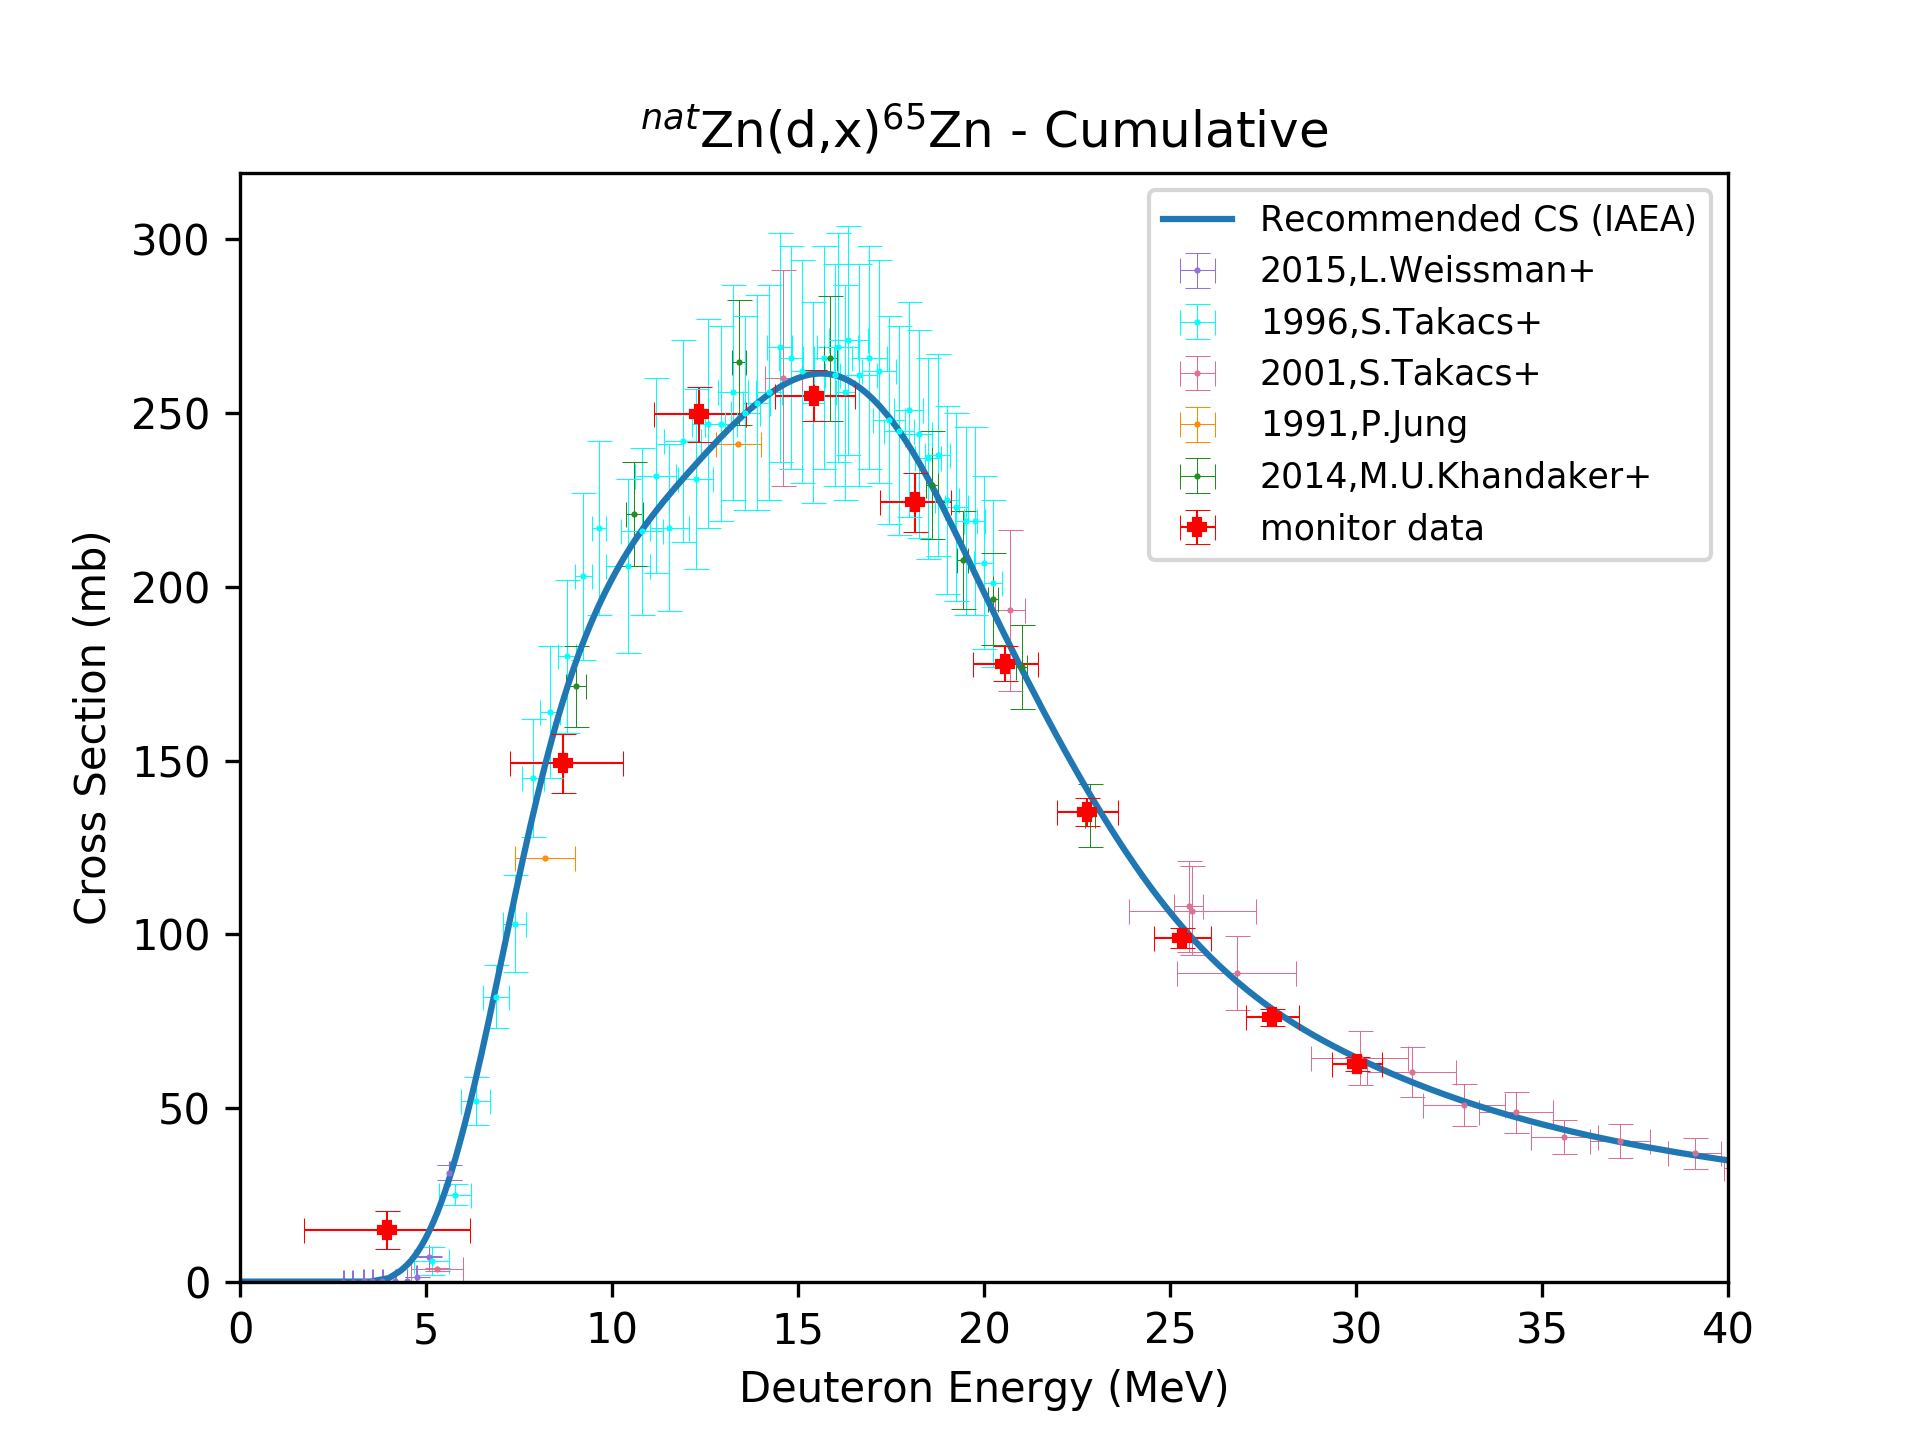
\includegraphics[width=5cm]{Cu_65Zn.png} }}%
    \quad
    \caption{Figure shows the estimation of monitor cross section using the calculated beam current. It is compared along with the monitor data.  }%
    \label{fig:monitor_BC}%
\end{figure}

\end{comment}